\chapter{Parte Experimental (In progress)}

En esta sección se realizará un análisis completo paso por paso del proceso de desarrollo del algoritmo. 
Se mostrarán distintas tablas y gráficas comparativas y sus interpretaciones con el fin de justificar la motivación de las distintas modificaciones introducidas explicadas en la sección anterior.

En primer lugar, recordemos brevemente los parámetros que utilizaremos y sus valores. 
Estos parámetros no necesitan ser introducidos manualmente al ejecutar el programa, si no que están definidos como constantes en el código:

\begin{itemize}
	\item \texttt{NTRIES}: Para eliminar la aleatoriedad que proviene de la ejecución con una determinada semilla u otra, cada algoritmo se ejecutará \texttt{NTRIES} número de veces, haremos la media de sus ejecuciones y este valor será el resultado que se guardará y se comparará posteriormente. 
	Para que los resultados puedan ser comparados estadísticamente, estableceremos su valor a 50.
	\item \texttt{INITSEED}: Con motivo de usar semillas distintas en cada ejecución del algoritmo, pero que los resultados sean replicables, se establece una semilla inicial \textit{hardcodeada} de forma arbitraria la cual va a generar el resto de semillas. 
	En nuestro caso, se ha elegido el valor 5. 
	\item \texttt{numcro}: Es el tamaño de la población de individuos que vamos a considerar en los algoritmos. 
	Se tiene que elegir un tamaño adecuado de forma que no sea demasiado grande, causando que se sobrepasen el límite de evaluaciones de forma prematura, ni demasiado pequeño, resultando en un incoveniente si se tiene que trabajar con muy pocos individuos. 
	Por lo tanto, estableceremos su valor a 10.
	\item \texttt{probc}: Es la probabilidad de cruce en los AGs. 
	No lo usamos como parámetro propiamente en el código, ya que para los algoritmos de referencia (AGE y CHC) tienen un número de cruces que se tienen que producir establecidos; en el caso de AGE solo se producirá un cruce por generación y para el CHC se intentarán cruzar todos los individuos posibles. 
	\item \texttt{probm}: Es la probabilidad de mutación en los AGs. Recuérdese que para el CHC no se requiere de esta mutación ya que obtiene la diversidad de otros operadores propios. 
	En la literatura se coincide que el valor de este parámetro debe ser uno bastante pequeño, generalmente entre un 1\% y un 10\% de la población. 
	Para asegurarnos que se produzca una mutación por cambio de generación, establecemos su valor a 0.1.
	\item \texttt{EvaluacionMAX}: Es el número de iteraciones/generaciones máximas. 
	Establecemos su valor a 450 por lo ya explicado en el apartado ``Diseño Experimental''.
	\item \texttt{seed}: Como se ha indicado anteriormente, cada ejecución individual de un algoritmo tendrá asociada una semilla para determinar la aleatoriedad de los acontecimientos y que sea replicable. 
	Este valor se tomará de aquellos que hayan sido generados por \texttt{INITSEED}.
\end{itemize}

Es importante mencionar que para todas las ejecuciones se han almacenado no solo los resultados finales, sino las mejores soluciones que se han encontrado en diversos momentos de la ejecución (\textit{milestones}). 
Es decir, se han almacenado las mejores soluciones encontradas en los porcentajes de ejecución $\{1,2,3,5,10,20,30,40,50,60,70,80,90,100\}$. 
Esto se podrá ver claramente cuando se muestren gráficas que representen de forma visual el \textit{ranking} de los distintos algoritmos comparados; sin embargo, por falta de espacio en las páginas y comodidad tanto para la autora como para el lector, en las tablas solo se mostrarán los resultados finales de las ejecuciones, aunque se harán menciones al comportamiento general (para determinar si puede estar convergiendo a una solución de forma prematura). 

Todos los códigos y resultados pueden ser encontrados en el \href{https://github.com/Itrilor/TFG/tree/main}{respositorio de Github de este trabajo}. 

\section{Algoritmos de Referencia experimentación}

Para empezar, debemos mostrar los resultados obtenidos de aplicar los algoritmos de referencia al problema con sus condiciones iniciales, esto es, con 90000 iteraciones en vez de 450. 


Preguntar si ha habido algún progreso con esto

\section{Resultados versión expensive}

Tal y como hemos mencionado en capítulos anteriores, el objetivo de este trabajo es el desarrollo de un algoritmo que ante todo sea capaz de obtener resultados competentes en poco tiempo, lo que se puede traducir en un número pequeño de iteraciones. 
Por lo que el siguiente paso será obtener los resultados para los mismos algoritmos que en la sección anterior, pero para su versión \textit{expensive}, es decir, utilizaremos un número de iteraciones máximas de 450, tal y como hemos establecido en los parámetros. 

Obtener resultados para esta versión es fundamental, ya que nos aporta las bases sobre las que trabajaremos y necesitaremos mejorar todo los posible durante este desarrollo. 
También es interesante observar lo mucho que empeoran los resultados frente a su versión normal, lo cual era de esperar, ya que recordemos que solo estamos utilizando el primer 0.5\% de las iteraciones de su versión original. 

Por ello, en la tabla \ref{AGEU450}, se muestran los resultados de la ejecución del AGE, mientras que en la tabla \ref{CHC450}, se muestran los resultados de la ejecución del CHC. 

Cabe mencionar que originalmente el único algoritmo de referencia que se consideró era el AG. 
Sin embargo, durante el desarrollo se consideró la posibilidad de introducir elementos propios del algoritmo CHC, ya que es un algoritmo bastante balanceado que suele dar buenos resultados. 
Por ello, también se realizó una comparación entre los resultados obtenidos por el AG y los del CHC. 
Esta comparación se puede apreciar en la gráfica \ref{fig:AGEUvsCHC}.


\begin{table}[]
\begin{tabular}{|cccccclll}
\hline
\rowcolor[HTML]{FFFFC7} 
\multicolumn{9}{|c|}{\cellcolor[HTML]{FFFFC7}AGEU   450}                                                                                                                                                                                                                                                                                                                                                                                                                                                                                                                                                                               \\ \hline
\rowcolor[HTML]{FCE6AB} 
\multicolumn{1}{|c|}{\cellcolor[HTML]{FCE6AB}n}                               & \multicolumn{1}{c|}{\cellcolor[HTML]{FCE6AB}densidad}              & \multicolumn{1}{c|}{\cellcolor[HTML]{FCE6AB}Resultado} & \multicolumn{1}{c|}{\cellcolor[HTML]{FCE6AB}n}                               & \multicolumn{1}{c|}{\cellcolor[HTML]{FCE6AB}densidad}               & \multicolumn{1}{c|}{\cellcolor[HTML]{FCE6AB}Resultado} & \multicolumn{1}{c|}{\cellcolor[HTML]{FCE6AB}n}                               & \multicolumn{1}{c|}{\cellcolor[HTML]{FCE6AB}densidad}              & \multicolumn{1}{c|}{\cellcolor[HTML]{FCE6AB}Resultado} \\ \hline
\rowcolor[HTML]{DAE8FC} 
\multicolumn{1}{|c|}{\cellcolor[HTML]{FFFFC7}}                                & \multicolumn{1}{c|}{\cellcolor[HTML]{DAE8FC}}                      & \multicolumn{1}{c|}{\cellcolor[HTML]{DAE8FC}192975}    & \multicolumn{1}{c|}{\cellcolor[HTML]{FFFFC7}}                                & \multicolumn{1}{c|}{\cellcolor[HTML]{DAE8FC}}                       & \multicolumn{1}{c|}{\cellcolor[HTML]{DAE8FC}375031}    & \multicolumn{1}{c|}{\cellcolor[HTML]{FFFFC7}}                                & \multicolumn{1}{c|}{\cellcolor[HTML]{DAE8FC}}                      & \multicolumn{1}{c|}{\cellcolor[HTML]{DAE8FC}376494}    \\ \cline{3-3} \cline{6-6} \cline{9-9} 
\multicolumn{1}{|c|}{\cellcolor[HTML]{FFFFC7}}                                & \multicolumn{1}{c|}{\cellcolor[HTML]{DAE8FC}}                      & \multicolumn{1}{c|}{\cellcolor[HTML]{DDFDFF}81641.3}   & \multicolumn{1}{c|}{\cellcolor[HTML]{FFFFC7}}                                & \multicolumn{1}{c|}{\cellcolor[HTML]{DAE8FC}}                       & \multicolumn{1}{c|}{\cellcolor[HTML]{DDFDFF}936531}    & \multicolumn{1}{c|}{\cellcolor[HTML]{FFFFC7}}                                & \multicolumn{1}{c|}{\cellcolor[HTML]{DAE8FC}}                      & \multicolumn{1}{c|}{\cellcolor[HTML]{DDFDFF}28788.7}   \\ \cline{3-3} \cline{6-6} \cline{9-9} 
\rowcolor[HTML]{DAE8FC} 
\multicolumn{1}{|c|}{\cellcolor[HTML]{FFFFC7}}                                & \multicolumn{1}{c|}{\cellcolor[HTML]{DAE8FC}}                      & \multicolumn{1}{c|}{\cellcolor[HTML]{DAE8FC}189162}    & \multicolumn{1}{c|}{\cellcolor[HTML]{FFFFC7}}                                & \multicolumn{1}{c|}{\cellcolor[HTML]{DAE8FC}}                       & \multicolumn{1}{c|}{\cellcolor[HTML]{DAE8FC}302452}    & \multicolumn{1}{c|}{\cellcolor[HTML]{FFFFC7}}                                & \multicolumn{1}{c|}{\cellcolor[HTML]{DAE8FC}}                      & \multicolumn{1}{c|}{\cellcolor[HTML]{DAE8FC}275573}    \\ \cline{3-3} \cline{6-6} \cline{9-9} 
\multicolumn{1}{|c|}{\cellcolor[HTML]{FFFFC7}}                                & \multicolumn{1}{c|}{\cellcolor[HTML]{DAE8FC}}                      & \multicolumn{1}{c|}{\cellcolor[HTML]{DDFDFF}224189}    & \multicolumn{1}{c|}{\cellcolor[HTML]{FFFFC7}}                                & \multicolumn{1}{c|}{\cellcolor[HTML]{DAE8FC}}                       & \multicolumn{1}{c|}{\cellcolor[HTML]{DDFDFF}29203.7}   & \multicolumn{1}{c|}{\cellcolor[HTML]{FFFFC7}}                                & \multicolumn{1}{c|}{\cellcolor[HTML]{DAE8FC}}                      & \multicolumn{1}{c|}{\cellcolor[HTML]{DDFDFF}439862}    \\ \cline{3-3} \cline{6-6} \cline{9-9} 
\rowcolor[HTML]{DAE8FC} 
\multicolumn{1}{|c|}{\cellcolor[HTML]{FFFFC7}}                                & \multicolumn{1}{c|}{\cellcolor[HTML]{DAE8FC}}                      & \multicolumn{1}{c|}{\cellcolor[HTML]{DAE8FC}229585}    & \multicolumn{1}{c|}{\cellcolor[HTML]{FFFFC7}}                                & \multicolumn{1}{c|}{\cellcolor[HTML]{DAE8FC}}                       & \multicolumn{1}{c|}{\cellcolor[HTML]{DAE8FC}100514}    & \multicolumn{1}{c|}{\cellcolor[HTML]{FFFFC7}}                                & \multicolumn{1}{c|}{\cellcolor[HTML]{DAE8FC}}                      & \multicolumn{1}{c|}{\cellcolor[HTML]{DAE8FC}14777.8}   \\ \cline{3-3} \cline{6-6} \cline{9-9} 
\multicolumn{1}{|c|}{\cellcolor[HTML]{FFFFC7}}                                & \multicolumn{1}{c|}{\cellcolor[HTML]{DAE8FC}}                      & \multicolumn{1}{c|}{\cellcolor[HTML]{DDFDFF}73991.5}   & \multicolumn{1}{c|}{\cellcolor[HTML]{FFFFC7}}                                & \multicolumn{1}{c|}{\cellcolor[HTML]{DAE8FC}}                       & \multicolumn{1}{c|}{\cellcolor[HTML]{DDFDFF}779113}    & \multicolumn{1}{c|}{\cellcolor[HTML]{FFFFC7}}                                & \multicolumn{1}{c|}{\cellcolor[HTML]{DAE8FC}}                      & \multicolumn{1}{c|}{\cellcolor[HTML]{DDFDFF}263938}    \\ \cline{3-3} \cline{6-6} \cline{9-9} 
\rowcolor[HTML]{DAE8FC} 
\multicolumn{1}{|c|}{\cellcolor[HTML]{FFFFC7}}                                & \multicolumn{1}{c|}{\cellcolor[HTML]{DAE8FC}}                      & \multicolumn{1}{c|}{\cellcolor[HTML]{DAE8FC}10154.9}   & \multicolumn{1}{c|}{\cellcolor[HTML]{FFFFC7}}                                & \multicolumn{1}{c|}{\cellcolor[HTML]{DAE8FC}}                       & \multicolumn{1}{c|}{\cellcolor[HTML]{DAE8FC}40194.9}   & \multicolumn{1}{c|}{\cellcolor[HTML]{FFFFC7}}                                & \multicolumn{1}{c|}{\cellcolor[HTML]{DAE8FC}}                      & \multicolumn{1}{c|}{\cellcolor[HTML]{DAE8FC}481905}    \\ \cline{3-3} \cline{6-6} \cline{9-9} 
\multicolumn{1}{|c|}{\cellcolor[HTML]{FFFFC7}}                                & \multicolumn{1}{c|}{\cellcolor[HTML]{DAE8FC}}                      & \multicolumn{1}{c|}{\cellcolor[HTML]{DDFDFF}62289.6}   & \multicolumn{1}{c|}{\cellcolor[HTML]{FFFFC7}}                                & \multicolumn{1}{c|}{\cellcolor[HTML]{DAE8FC}}                       & \multicolumn{1}{c|}{\cellcolor[HTML]{DDFDFF}693305}    & \multicolumn{1}{c|}{\cellcolor[HTML]{FFFFC7}}                                & \multicolumn{1}{c|}{\cellcolor[HTML]{DAE8FC}}                      & \multicolumn{1}{c|}{\cellcolor[HTML]{DDFDFF}9176.36}   \\ \cline{3-3} \cline{6-6} \cline{9-9} 
\rowcolor[HTML]{DAE8FC} 
\multicolumn{1}{|c|}{\cellcolor[HTML]{FFFFC7}}                                & \multicolumn{1}{c|}{\cellcolor[HTML]{DAE8FC}}                      & \multicolumn{1}{c|}{\cellcolor[HTML]{DAE8FC}232572}    & \multicolumn{1}{c|}{\cellcolor[HTML]{FFFFC7}}                                & \multicolumn{1}{c|}{\multirow{-9}{*}{\cellcolor[HTML]{DAE8FC}25}}   & \multicolumn{1}{c|}{\cellcolor[HTML]{DAE8FC}779359}    & \multicolumn{1}{c|}{\cellcolor[HTML]{FFFFC7}}                                & \multicolumn{1}{c|}{\multirow{-9}{*}{\cellcolor[HTML]{DAE8FC}25}}  & \multicolumn{1}{c|}{\cellcolor[HTML]{DAE8FC}245377}    \\ \cline{3-3} \cline{5-6} \cline{8-9} 
\multicolumn{1}{|c|}{\cellcolor[HTML]{FFFFC7}}                                & \multicolumn{1}{c|}{\multirow{-10}{*}{\cellcolor[HTML]{DAE8FC}25}} & \multicolumn{1}{c|}{\cellcolor[HTML]{DDFDFF}24729.5}   & \multicolumn{1}{c|}{\cellcolor[HTML]{FFFFC7}}                                & \multicolumn{1}{c|}{\cellcolor[HTML]{DDFDFF}}                       & \multicolumn{1}{c|}{\cellcolor[HTML]{DAE8FC}622413}    & \multicolumn{1}{c|}{\cellcolor[HTML]{FFFFC7}}                                & \multicolumn{1}{c|}{\cellcolor[HTML]{DDFDFF}}                      & \multicolumn{1}{c|}{\cellcolor[HTML]{DAE8FC}990137}    \\ \cline{2-3} \cline{6-6} \cline{9-9} 
\rowcolor[HTML]{DDFDFF} 
\multicolumn{1}{|c|}{\cellcolor[HTML]{FFFFC7}}                                & \multicolumn{1}{c|}{\cellcolor[HTML]{DDFDFF}}                      & \multicolumn{1}{c|}{\cellcolor[HTML]{DAE8FC}18382.8}   & \multicolumn{1}{c|}{\cellcolor[HTML]{FFFFC7}}                                & \multicolumn{1}{c|}{\cellcolor[HTML]{DDFDFF}}                       & \multicolumn{1}{c|}{\cellcolor[HTML]{DDFDFF}47981}     & \multicolumn{1}{c|}{\cellcolor[HTML]{FFFFC7}}                                & \multicolumn{1}{c|}{\cellcolor[HTML]{DDFDFF}}                      & \multicolumn{1}{c|}{\cellcolor[HTML]{DDFDFF}501953}    \\ \cline{3-3} \cline{6-6} \cline{9-9} 
\multicolumn{1}{|c|}{\cellcolor[HTML]{FFFFC7}}                                & \multicolumn{1}{c|}{\cellcolor[HTML]{DDFDFF}}                      & \multicolumn{1}{c|}{\cellcolor[HTML]{DDFDFF}56493.1}   & \multicolumn{1}{c|}{\cellcolor[HTML]{FFFFC7}}                                & \multicolumn{1}{c|}{\cellcolor[HTML]{DDFDFF}}                       & \multicolumn{1}{c|}{\cellcolor[HTML]{DAE8FC}203099}    & \multicolumn{1}{c|}{\cellcolor[HTML]{FFFFC7}}                                & \multicolumn{1}{c|}{\cellcolor[HTML]{DDFDFF}}                      & \multicolumn{1}{c|}{\cellcolor[HTML]{DAE8FC}104754}    \\ \cline{3-3} \cline{6-6} \cline{9-9} 
\rowcolor[HTML]{DDFDFF} 
\multicolumn{1}{|c|}{\cellcolor[HTML]{FFFFC7}}                                & \multicolumn{1}{c|}{\cellcolor[HTML]{DDFDFF}}                      & \multicolumn{1}{c|}{\cellcolor[HTML]{DAE8FC}3703.2}    & \multicolumn{1}{c|}{\cellcolor[HTML]{FFFFC7}}                                & \multicolumn{1}{c|}{\cellcolor[HTML]{DDFDFF}}                       & \multicolumn{1}{c|}{\cellcolor[HTML]{DDFDFF}239245}    & \multicolumn{1}{c|}{\cellcolor[HTML]{FFFFC7}}                                & \multicolumn{1}{c|}{\cellcolor[HTML]{DDFDFF}}                      & \multicolumn{1}{c|}{\cellcolor[HTML]{DDFDFF}866729}    \\ \cline{3-3} \cline{6-6} \cline{9-9} 
\multicolumn{1}{|c|}{\cellcolor[HTML]{FFFFC7}}                                & \multicolumn{1}{c|}{\cellcolor[HTML]{DDFDFF}}                      & \multicolumn{1}{c|}{\cellcolor[HTML]{DDFDFF}50077.8}   & \multicolumn{1}{c|}{\cellcolor[HTML]{FFFFC7}}                                & \multicolumn{1}{c|}{\cellcolor[HTML]{DDFDFF}}                       & \multicolumn{1}{c|}{\cellcolor[HTML]{DAE8FC}220724}    & \multicolumn{1}{c|}{\cellcolor[HTML]{FFFFC7}}                                & \multicolumn{1}{c|}{\cellcolor[HTML]{DDFDFF}}                      & \multicolumn{1}{c|}{\cellcolor[HTML]{DAE8FC}301858}    \\ \cline{3-3} \cline{6-6} \cline{9-9} 
\rowcolor[HTML]{DDFDFF} 
\multicolumn{1}{|c|}{\cellcolor[HTML]{FFFFC7}}                                & \multicolumn{1}{c|}{\cellcolor[HTML]{DDFDFF}}                      & \multicolumn{1}{c|}{\cellcolor[HTML]{DAE8FC}61451.4}   & \multicolumn{1}{c|}{\cellcolor[HTML]{FFFFC7}}                                & \multicolumn{1}{c|}{\cellcolor[HTML]{DDFDFF}}                       & \multicolumn{1}{c|}{\cellcolor[HTML]{DDFDFF}185943}    & \multicolumn{1}{c|}{\cellcolor[HTML]{FFFFC7}}                                & \multicolumn{1}{c|}{\cellcolor[HTML]{DDFDFF}}                      & \multicolumn{1}{c|}{\cellcolor[HTML]{DDFDFF}716621}    \\ \cline{3-3} \cline{6-6} \cline{9-9} 
\multicolumn{1}{|c|}{\cellcolor[HTML]{FFFFC7}}                                & \multicolumn{1}{c|}{\cellcolor[HTML]{DDFDFF}}                      & \multicolumn{1}{c|}{\cellcolor[HTML]{DDFDFF}35971.6}   & \multicolumn{1}{c|}{\cellcolor[HTML]{FFFFC7}}                                & \multicolumn{1}{c|}{\cellcolor[HTML]{DDFDFF}}                       & \multicolumn{1}{c|}{\cellcolor[HTML]{DAE8FC}79424.5}   & \multicolumn{1}{c|}{\cellcolor[HTML]{FFFFC7}}                                & \multicolumn{1}{c|}{\cellcolor[HTML]{DDFDFF}}                      & \multicolumn{1}{c|}{\cellcolor[HTML]{DAE8FC}722726}    \\ \cline{3-3} \cline{6-6} \cline{9-9} 
\rowcolor[HTML]{DDFDFF} 
\multicolumn{1}{|c|}{\cellcolor[HTML]{FFFFC7}}                                & \multicolumn{1}{c|}{\cellcolor[HTML]{DDFDFF}}                      & \multicolumn{1}{c|}{\cellcolor[HTML]{DAE8FC}14528.2}   & \multicolumn{1}{c|}{\cellcolor[HTML]{FFFFC7}}                                & \multicolumn{1}{c|}{\cellcolor[HTML]{DDFDFF}}                       & \multicolumn{1}{c|}{\cellcolor[HTML]{DDFDFF}58364.2}   & \multicolumn{1}{c|}{\cellcolor[HTML]{FFFFC7}}                                & \multicolumn{1}{c|}{\cellcolor[HTML]{DDFDFF}}                      & \multicolumn{1}{c|}{\cellcolor[HTML]{DDFDFF}43401.7}   \\ \cline{3-3} \cline{6-6} \cline{9-9} 
\multicolumn{1}{|c|}{\cellcolor[HTML]{FFFFC7}}                                & \multicolumn{1}{c|}{\cellcolor[HTML]{DDFDFF}}                      & \multicolumn{1}{c|}{\cellcolor[HTML]{DDFDFF}20289.4}   & \multicolumn{1}{c|}{\cellcolor[HTML]{FFFFC7}}                                & \multicolumn{1}{c|}{\cellcolor[HTML]{DDFDFF}}                       & \multicolumn{1}{c|}{\cellcolor[HTML]{DAE8FC}147914}    & \multicolumn{1}{c|}{\cellcolor[HTML]{FFFFC7}}                                & \multicolumn{1}{c|}{\cellcolor[HTML]{DDFDFF}}                      & \multicolumn{1}{c|}{\cellcolor[HTML]{DAE8FC}756135}    \\ \cline{3-3} \cline{6-6} \cline{9-9} 
\rowcolor[HTML]{DDFDFF} 
\multicolumn{1}{|c|}{\cellcolor[HTML]{FFFFC7}}                                & \multicolumn{1}{c|}{\cellcolor[HTML]{DDFDFF}}                      & \multicolumn{1}{c|}{\cellcolor[HTML]{DAE8FC}35073.3}   & \multicolumn{1}{c|}{\cellcolor[HTML]{FFFFC7}}                                & \multicolumn{1}{c|}{\multirow{-10}{*}{\cellcolor[HTML]{DDFDFF}50}}  & \multicolumn{1}{c|}{\cellcolor[HTML]{DDFDFF}48982.8}   & \multicolumn{1}{c|}{\multirow{-19}{*}{\cellcolor[HTML]{FFFFC7}\textbf{300}}} & \multicolumn{1}{c|}{\multirow{-10}{*}{\cellcolor[HTML]{DDFDFF}50}} & \multicolumn{1}{c|}{\cellcolor[HTML]{DDFDFF}751915}    \\ \cline{3-3} \cline{5-9} 
\multicolumn{1}{|c|}{\cellcolor[HTML]{FFFFC7}}                                & \multicolumn{1}{c|}{\multirow{-10}{*}{\cellcolor[HTML]{DDFDFF}50}} & \multicolumn{1}{c|}{\cellcolor[HTML]{DDFDFF}88195.5}   & \multicolumn{1}{c|}{\cellcolor[HTML]{FFFFC7}}                                & \multicolumn{1}{c|}{\cellcolor[HTML]{DAE8FC}}                       & \multicolumn{1}{c|}{\cellcolor[HTML]{DAE8FC}281677}    &                                                                              &                                                                    &                                                        \\ \cline{2-3} \cline{6-6}
\multicolumn{1}{|c|}{\cellcolor[HTML]{FFFFC7}}                                & \multicolumn{1}{c|}{\cellcolor[HTML]{DAE8FC}}                      & \multicolumn{1}{c|}{\cellcolor[HTML]{DAE8FC}83363}     & \multicolumn{1}{c|}{\cellcolor[HTML]{FFFFC7}}                                & \multicolumn{1}{c|}{\cellcolor[HTML]{DAE8FC}}                       & \multicolumn{1}{c|}{\cellcolor[HTML]{DDFDFF}369024}    &                                                                              &                                                                    &                                                        \\ \cline{3-3} \cline{6-6}
\multicolumn{1}{|c|}{\cellcolor[HTML]{FFFFC7}}                                & \multicolumn{1}{c|}{\cellcolor[HTML]{DAE8FC}}                      & \multicolumn{1}{c|}{\cellcolor[HTML]{DDFDFF}104674}    & \multicolumn{1}{c|}{\cellcolor[HTML]{FFFFC7}}                                & \multicolumn{1}{c|}{\cellcolor[HTML]{DAE8FC}}                       & \multicolumn{1}{c|}{\cellcolor[HTML]{DAE8FC}209377}    &                                                                              &                                                                    &                                                        \\ \cline{3-3} \cline{6-6}
\multicolumn{1}{|c|}{\cellcolor[HTML]{FFFFC7}}                                & \multicolumn{1}{c|}{\cellcolor[HTML]{DAE8FC}}                      & \multicolumn{1}{c|}{\cellcolor[HTML]{DAE8FC}33684.2}   & \multicolumn{1}{c|}{\cellcolor[HTML]{FFFFC7}}                                & \multicolumn{1}{c|}{\cellcolor[HTML]{DAE8FC}}                       & \multicolumn{1}{c|}{\cellcolor[HTML]{DDFDFF}225289}    &                                                                              &                                                                    &                                                        \\ \cline{3-3} \cline{6-6}
\multicolumn{1}{|c|}{\cellcolor[HTML]{FFFFC7}}                                & \multicolumn{1}{c|}{\cellcolor[HTML]{DAE8FC}}                      & \multicolumn{1}{c|}{\cellcolor[HTML]{DDFDFF}105760}    & \multicolumn{1}{c|}{\cellcolor[HTML]{FFFFC7}}                                & \multicolumn{1}{c|}{\cellcolor[HTML]{DAE8FC}}                       & \multicolumn{1}{c|}{\cellcolor[HTML]{DAE8FC}225869}    &                                                                              &                                                                    &                                                        \\ \cline{3-3} \cline{6-6}
\multicolumn{1}{|c|}{\cellcolor[HTML]{FFFFC7}}                                & \multicolumn{1}{c|}{\cellcolor[HTML]{DAE8FC}}                      & \multicolumn{1}{c|}{\cellcolor[HTML]{DAE8FC}56123.2}   & \multicolumn{1}{c|}{\cellcolor[HTML]{FFFFC7}}                                & \multicolumn{1}{c|}{\cellcolor[HTML]{DAE8FC}}                       & \multicolumn{1}{c|}{\cellcolor[HTML]{DDFDFF}479039}    &                                                                              &                                                                    &                                                        \\ \cline{3-3} \cline{6-6}
\multicolumn{1}{|c|}{\cellcolor[HTML]{FFFFC7}}                                & \multicolumn{1}{c|}{\cellcolor[HTML]{DAE8FC}}                      & \multicolumn{1}{c|}{\cellcolor[HTML]{DDFDFF}16040.6}   & \multicolumn{1}{c|}{\cellcolor[HTML]{FFFFC7}}                                & \multicolumn{1}{c|}{\cellcolor[HTML]{DAE8FC}}                       & \multicolumn{1}{c|}{\cellcolor[HTML]{DAE8FC}425768}    &                                                                              &                                                                    &                                                        \\ \cline{3-3} \cline{6-6}
\multicolumn{1}{|c|}{\cellcolor[HTML]{FFFFC7}}                                & \multicolumn{1}{c|}{\cellcolor[HTML]{DAE8FC}}                      & \multicolumn{1}{c|}{\cellcolor[HTML]{DAE8FC}52535.1}   & \multicolumn{1}{c|}{\cellcolor[HTML]{FFFFC7}}                                & \multicolumn{1}{c|}{\cellcolor[HTML]{DAE8FC}}                       & \multicolumn{1}{c|}{\cellcolor[HTML]{DDFDFF}218123}    &                                                                              &                                                                    &                                                        \\ \cline{3-3} \cline{6-6}
\multicolumn{1}{|c|}{\cellcolor[HTML]{FFFFC7}}                                & \multicolumn{1}{c|}{\cellcolor[HTML]{DAE8FC}}                      & \multicolumn{1}{c|}{\cellcolor[HTML]{DDFDFF}53964}     & \multicolumn{1}{c|}{\cellcolor[HTML]{FFFFC7}}                                & \multicolumn{1}{c|}{\cellcolor[HTML]{DAE8FC}}                       & \multicolumn{1}{c|}{\cellcolor[HTML]{DAE8FC}315253}    &                                                                              &                                                                    &                                                        \\ \cline{3-3} \cline{6-6}
\multicolumn{1}{|c|}{\cellcolor[HTML]{FFFFC7}}                                & \multicolumn{1}{c|}{\cellcolor[HTML]{DAE8FC}}                      & \multicolumn{1}{c|}{\cellcolor[HTML]{DAE8FC}68468.1}   & \multicolumn{1}{c|}{\cellcolor[HTML]{FFFFC7}}                                & \multicolumn{1}{c|}{\multirow{-10}{*}{\cellcolor[HTML]{DAE8FC}75}}  & \multicolumn{1}{c|}{\cellcolor[HTML]{DDFDFF}104110}    &                                                                              &                                                                    &                                                        \\ \cline{3-3} \cline{5-6}
\multicolumn{1}{|c|}{\cellcolor[HTML]{FFFFC7}}                                & \multicolumn{1}{c|}{\multirow{-10}{*}{\cellcolor[HTML]{DAE8FC}75}} & \multicolumn{1}{c|}{\cellcolor[HTML]{DDFDFF}143555}    & \multicolumn{1}{c|}{\cellcolor[HTML]{FFFFC7}}                                & \multicolumn{1}{c|}{\cellcolor[HTML]{DDFDFF}}                       & \multicolumn{1}{c|}{\cellcolor[HTML]{DAE8FC}142039}    &                                                                              &                                                                    &                                                        \\ \cline{2-3} \cline{6-6}
\multicolumn{1}{|c|}{\cellcolor[HTML]{FFFFC7}}                                & \multicolumn{1}{c|}{\cellcolor[HTML]{DDFDFF}}                      & \multicolumn{1}{c|}{\cellcolor[HTML]{DAE8FC}188657}    & \multicolumn{1}{c|}{\cellcolor[HTML]{FFFFC7}}                                & \multicolumn{1}{c|}{\cellcolor[HTML]{DDFDFF}}                       & \multicolumn{1}{c|}{\cellcolor[HTML]{DDFDFF}439482}    &                                                                              &                                                                    &                                                        \\ \cline{3-3} \cline{6-6}
\multicolumn{1}{|c|}{\cellcolor[HTML]{FFFFC7}}                                & \multicolumn{1}{c|}{\cellcolor[HTML]{DDFDFF}}                      & \multicolumn{1}{c|}{\cellcolor[HTML]{DDFDFF}94679.5}   & \multicolumn{1}{c|}{\cellcolor[HTML]{FFFFC7}}                                & \multicolumn{1}{c|}{\cellcolor[HTML]{DDFDFF}}                       & \multicolumn{1}{c|}{\cellcolor[HTML]{DAE8FC}283241}    &                                                                              &                                                                    &                                                        \\ \cline{3-3} \cline{6-6}
\multicolumn{1}{|c|}{\cellcolor[HTML]{FFFFC7}}                                & \multicolumn{1}{c|}{\cellcolor[HTML]{DDFDFF}}                      & \multicolumn{1}{c|}{\cellcolor[HTML]{DAE8FC}61561.5}   & \multicolumn{1}{c|}{\cellcolor[HTML]{FFFFC7}}                                & \multicolumn{1}{c|}{\cellcolor[HTML]{DDFDFF}}                       & \multicolumn{1}{c|}{\cellcolor[HTML]{DDFDFF}61605.9}   &                                                                              &                                                                    &                                                        \\ \cline{3-3} \cline{6-6}
\multicolumn{1}{|c|}{\cellcolor[HTML]{FFFFC7}}                                & \multicolumn{1}{c|}{\cellcolor[HTML]{DDFDFF}}                      & \multicolumn{1}{c|}{\cellcolor[HTML]{DDFDFF}71896.1}   & \multicolumn{1}{c|}{\cellcolor[HTML]{FFFFC7}}                                & \multicolumn{1}{c|}{\cellcolor[HTML]{DDFDFF}}                       & \multicolumn{1}{c|}{\cellcolor[HTML]{DAE8FC}127029}    &                                                                              &                                                                    &                                                        \\ \cline{3-3} \cline{6-6}
\multicolumn{1}{|c|}{\cellcolor[HTML]{FFFFC7}}                                & \multicolumn{1}{c|}{\cellcolor[HTML]{DDFDFF}}                      & \multicolumn{1}{c|}{\cellcolor[HTML]{DAE8FC}27565.6}   & \multicolumn{1}{c|}{\cellcolor[HTML]{FFFFC7}}                                & \multicolumn{1}{c|}{\cellcolor[HTML]{DDFDFF}}                       & \multicolumn{1}{c|}{\cellcolor[HTML]{DDFDFF}137458}    &                                                                              &                                                                    &                                                        \\ \cline{3-3} \cline{6-6}
\multicolumn{1}{|c|}{\cellcolor[HTML]{FFFFC7}}                                & \multicolumn{1}{c|}{\cellcolor[HTML]{DDFDFF}}                      & \multicolumn{1}{c|}{\cellcolor[HTML]{DDFDFF}144945}    & \multicolumn{1}{c|}{\cellcolor[HTML]{FFFFC7}}                                & \multicolumn{1}{c|}{\cellcolor[HTML]{DDFDFF}}                       & \multicolumn{1}{c|}{\cellcolor[HTML]{DAE8FC}228081}    &                                                                              &                                                                    &                                                        \\ \cline{3-3} \cline{6-6}
\multicolumn{1}{|c|}{\cellcolor[HTML]{FFFFC7}}                                & \multicolumn{1}{c|}{\cellcolor[HTML]{DDFDFF}}                      & \multicolumn{1}{c|}{\cellcolor[HTML]{DAE8FC}110542}    & \multicolumn{1}{c|}{\cellcolor[HTML]{FFFFC7}}                                & \multicolumn{1}{c|}{\cellcolor[HTML]{DDFDFF}}                       & \multicolumn{1}{c|}{\cellcolor[HTML]{DDFDFF}267388}    &                                                                              &                                                                    &                                                        \\ \cline{3-3} \cline{6-6}
\multicolumn{1}{|c|}{\cellcolor[HTML]{FFFFC7}}                                & \multicolumn{1}{c|}{\cellcolor[HTML]{DDFDFF}}                      & \multicolumn{1}{c|}{\cellcolor[HTML]{DDFDFF}19419}     & \multicolumn{1}{c|}{\cellcolor[HTML]{FFFFC7}}                                & \multicolumn{1}{c|}{\cellcolor[HTML]{DDFDFF}}                       & \multicolumn{1}{c|}{\cellcolor[HTML]{DAE8FC}596574}    &                                                                              &                                                                    &                                                        \\ \cline{3-3} \cline{6-6}
\multicolumn{1}{|c|}{\multirow{-39}{*}{\cellcolor[HTML]{FFFFC7}\textbf{100}}} & \multicolumn{1}{c|}{\multirow{-9}{*}{\cellcolor[HTML]{DDFDFF}100}} & \multicolumn{1}{c|}{\cellcolor[HTML]{DAE8FC}103743}    & \multicolumn{1}{c|}{\multirow{-39}{*}{\cellcolor[HTML]{FFFFC7}\textbf{200}}} & \multicolumn{1}{c|}{\multirow{-10}{*}{\cellcolor[HTML]{DDFDFF}100}} & \multicolumn{1}{c|}{\cellcolor[HTML]{DDFDFF}512266}    &                                                                              &                                                                    &                                                        \\ \cline{1-6}
\end{tabular}
\caption{\label{AGEU450}Resultados de la ejecución de AGEU con 450 iteraciones}
\end{table}

% Please add the following required packages to your document preamble:
% \usepackage{multirow}
% \usepackage[table,xcdraw]{xcolor}
% If you use beamer only pass "xcolor=table" option, i.e. \documentclass[xcolor=table]{beamer}
\begin{table}[]
\begin{tabular}{|cclccllll}
\hline
\rowcolor[HTML]{FFFFC7} 
\multicolumn{9}{|c|}{\cellcolor[HTML]{FFFFC7}CHC   450}                                                                                                                                                                                                                                                                                                                                                                                                                                                                                                                                                                                \\ \hline
\rowcolor[HTML]{F7EAC7} 
\multicolumn{1}{|c|}{\cellcolor[HTML]{F7EAC7}n}                               & \multicolumn{1}{c|}{\cellcolor[HTML]{F7EAC7}densidad}              & \multicolumn{1}{c|}{\cellcolor[HTML]{F7EAC7}Resultado} & \multicolumn{1}{c|}{\cellcolor[HTML]{F7EAC7}n}                               & \multicolumn{1}{c|}{\cellcolor[HTML]{F7EAC7}densidad}               & \multicolumn{1}{c|}{\cellcolor[HTML]{F7EAC7}Resultado} & \multicolumn{1}{c|}{\cellcolor[HTML]{F7EAC7}n}                               & \multicolumn{1}{c|}{\cellcolor[HTML]{F7EAC7}densidad}              & \multicolumn{1}{c|}{\cellcolor[HTML]{F7EAC7}Resultado} \\ \hline
\rowcolor[HTML]{DAE8FC} 
\multicolumn{1}{|c|}{\cellcolor[HTML]{FFFFC7}}                                & \multicolumn{1}{c|}{\cellcolor[HTML]{DAE8FC}}                      & \multicolumn{1}{l|}{\cellcolor[HTML]{DAE8FC}191858}    & \multicolumn{1}{c|}{\cellcolor[HTML]{FFFFC7}}                                & \multicolumn{1}{c|}{\cellcolor[HTML]{DAE8FC}}                       & \multicolumn{1}{l|}{\cellcolor[HTML]{DAE8FC}372331}    & \multicolumn{1}{c|}{\cellcolor[HTML]{FFFFC7}}                                & \multicolumn{1}{c|}{\cellcolor[HTML]{DAE8FC}}                      & \multicolumn{1}{l|}{\cellcolor[HTML]{DAE8FC}371526}    \\ \cline{3-3} \cline{6-6} \cline{9-9} 
\multicolumn{1}{|c|}{\cellcolor[HTML]{FFFFC7}}                                & \multicolumn{1}{c|}{\cellcolor[HTML]{DAE8FC}}                      & \multicolumn{1}{l|}{\cellcolor[HTML]{DDFDFF}81329.3}   & \multicolumn{1}{c|}{\cellcolor[HTML]{FFFFC7}}                                & \multicolumn{1}{c|}{\cellcolor[HTML]{DAE8FC}}                       & \multicolumn{1}{l|}{\cellcolor[HTML]{DDFDFF}934965}    & \multicolumn{1}{c|}{\cellcolor[HTML]{FFFFC7}}                                & \multicolumn{1}{c|}{\cellcolor[HTML]{DAE8FC}}                      & \multicolumn{1}{l|}{\cellcolor[HTML]{DDFDFF}28637.6}   \\ \cline{3-3} \cline{6-6} \cline{9-9} 
\rowcolor[HTML]{DAE8FC} 
\multicolumn{1}{|c|}{\cellcolor[HTML]{FFFFC7}}                                & \multicolumn{1}{c|}{\cellcolor[HTML]{DAE8FC}}                      & \multicolumn{1}{l|}{\cellcolor[HTML]{DAE8FC}188291}    & \multicolumn{1}{c|}{\cellcolor[HTML]{FFFFC7}}                                & \multicolumn{1}{c|}{\cellcolor[HTML]{DAE8FC}}                       & \multicolumn{1}{l|}{\cellcolor[HTML]{DAE8FC}299738}    & \multicolumn{1}{c|}{\cellcolor[HTML]{FFFFC7}}                                & \multicolumn{1}{c|}{\cellcolor[HTML]{DAE8FC}}                      & \multicolumn{1}{l|}{\cellcolor[HTML]{DAE8FC}272165}    \\ \cline{3-3} \cline{6-6} \cline{9-9} 
\multicolumn{1}{|c|}{\cellcolor[HTML]{FFFFC7}}                                & \multicolumn{1}{c|}{\cellcolor[HTML]{DAE8FC}}                      & \multicolumn{1}{l|}{\cellcolor[HTML]{DDFDFF}223260}    & \multicolumn{1}{c|}{\cellcolor[HTML]{FFFFC7}}                                & \multicolumn{1}{c|}{\cellcolor[HTML]{DAE8FC}}                       & \multicolumn{1}{l|}{\cellcolor[HTML]{DDFDFF}28848.1}   & \multicolumn{1}{c|}{\cellcolor[HTML]{FFFFC7}}                                & \multicolumn{1}{c|}{\cellcolor[HTML]{DAE8FC}}                      & \multicolumn{1}{l|}{\cellcolor[HTML]{DDFDFF}434626}    \\ \cline{3-3} \cline{6-6} \cline{9-9} 
\rowcolor[HTML]{DAE8FC} 
\multicolumn{1}{|c|}{\cellcolor[HTML]{FFFFC7}}                                & \multicolumn{1}{c|}{\cellcolor[HTML]{DAE8FC}}                      & \multicolumn{1}{l|}{\cellcolor[HTML]{DAE8FC}228377}    & \multicolumn{1}{c|}{\cellcolor[HTML]{FFFFC7}}                                & \multicolumn{1}{c|}{\cellcolor[HTML]{DAE8FC}}                       & \multicolumn{1}{l|}{\cellcolor[HTML]{DAE8FC}99231.6}   & \multicolumn{1}{c|}{\cellcolor[HTML]{FFFFC7}}                                & \multicolumn{1}{c|}{\cellcolor[HTML]{DAE8FC}}                      & \multicolumn{1}{l|}{\cellcolor[HTML]{DAE8FC}14864.6}   \\ \cline{3-3} \cline{6-6} \cline{9-9} 
\multicolumn{1}{|c|}{\cellcolor[HTML]{FFFFC7}}                                & \multicolumn{1}{c|}{\cellcolor[HTML]{DAE8FC}}                      & \multicolumn{1}{l|}{\cellcolor[HTML]{DDFDFF}73621.4}   & \multicolumn{1}{c|}{\cellcolor[HTML]{FFFFC7}}                                & \multicolumn{1}{c|}{\cellcolor[HTML]{DAE8FC}}                       & \multicolumn{1}{l|}{\cellcolor[HTML]{DDFDFF}774945}    & \multicolumn{1}{c|}{\cellcolor[HTML]{FFFFC7}}                                & \multicolumn{1}{c|}{\cellcolor[HTML]{DAE8FC}}                      & \multicolumn{1}{l|}{\cellcolor[HTML]{DDFDFF}259391}    \\ \cline{3-3} \cline{6-6} \cline{9-9} 
\rowcolor[HTML]{DAE8FC} 
\multicolumn{1}{|c|}{\cellcolor[HTML]{FFFFC7}}                                & \multicolumn{1}{c|}{\cellcolor[HTML]{DAE8FC}}                      & \multicolumn{1}{l|}{\cellcolor[HTML]{DAE8FC}10099.3}   & \multicolumn{1}{c|}{\cellcolor[HTML]{FFFFC7}}                                & \multicolumn{1}{c|}{\cellcolor[HTML]{DAE8FC}}                       & \multicolumn{1}{l|}{\cellcolor[HTML]{DAE8FC}39613.1}   & \multicolumn{1}{c|}{\cellcolor[HTML]{FFFFC7}}                                & \multicolumn{1}{c|}{\cellcolor[HTML]{DAE8FC}}                      & \multicolumn{1}{l|}{\cellcolor[HTML]{DAE8FC}477525}    \\ \cline{3-3} \cline{6-6} \cline{9-9} 
\multicolumn{1}{|c|}{\cellcolor[HTML]{FFFFC7}}                                & \multicolumn{1}{c|}{\cellcolor[HTML]{DAE8FC}}                      & \multicolumn{1}{l|}{\cellcolor[HTML]{DDFDFF}61818.1}   & \multicolumn{1}{c|}{\cellcolor[HTML]{FFFFC7}}                                & \multicolumn{1}{c|}{\cellcolor[HTML]{DAE8FC}}                       & \multicolumn{1}{l|}{\cellcolor[HTML]{DDFDFF}689720}    & \multicolumn{1}{c|}{\cellcolor[HTML]{FFFFC7}}                                & \multicolumn{1}{c|}{\cellcolor[HTML]{DAE8FC}}                      & \multicolumn{1}{l|}{\cellcolor[HTML]{DDFDFF}9258.1}    \\ \cline{3-3} \cline{6-6} \cline{9-9} 
\rowcolor[HTML]{DAE8FC} 
\multicolumn{1}{|c|}{\cellcolor[HTML]{FFFFC7}}                                & \multicolumn{1}{c|}{\cellcolor[HTML]{DAE8FC}}                      & \multicolumn{1}{l|}{\cellcolor[HTML]{DAE8FC}231871}    & \multicolumn{1}{c|}{\cellcolor[HTML]{FFFFC7}}                                & \multicolumn{1}{c|}{\multirow{-9}{*}{\cellcolor[HTML]{DAE8FC}25}}   & \multicolumn{1}{l|}{\cellcolor[HTML]{DAE8FC}773943}    & \multicolumn{1}{c|}{\cellcolor[HTML]{FFFFC7}}                                & \multicolumn{1}{c|}{\multirow{-9}{*}{\cellcolor[HTML]{DAE8FC}25}}  & \multicolumn{1}{l|}{\cellcolor[HTML]{DAE8FC}240501}    \\ \cline{3-3} \cline{5-6} \cline{8-9} 
\multicolumn{1}{|c|}{\cellcolor[HTML]{FFFFC7}}                                & \multicolumn{1}{c|}{\multirow{-10}{*}{\cellcolor[HTML]{DAE8FC}25}} & \multicolumn{1}{l|}{\cellcolor[HTML]{DDFDFF}24609.9}   & \multicolumn{1}{c|}{\cellcolor[HTML]{FFFFC7}}                                & \multicolumn{1}{c|}{\cellcolor[HTML]{DDFDFF}}                       & \multicolumn{1}{l|}{\cellcolor[HTML]{DAE8FC}619791}    & \multicolumn{1}{c|}{\cellcolor[HTML]{FFFFC7}}                                & \multicolumn{1}{c|}{\cellcolor[HTML]{DDFDFF}}                      & \multicolumn{1}{l|}{\cellcolor[HTML]{DAE8FC}984358}    \\ \cline{2-3} \cline{6-6} \cline{9-9} 
\rowcolor[HTML]{DDFDFF} 
\multicolumn{1}{|c|}{\cellcolor[HTML]{FFFFC7}}                                & \multicolumn{1}{c|}{\cellcolor[HTML]{DDFDFF}}                      & \multicolumn{1}{l|}{\cellcolor[HTML]{DAE8FC}18473.4}   & \multicolumn{1}{c|}{\cellcolor[HTML]{FFFFC7}}                                & \multicolumn{1}{c|}{\cellcolor[HTML]{DDFDFF}}                       & \multicolumn{1}{l|}{\cellcolor[HTML]{DDFDFF}47923.5}   & \multicolumn{1}{c|}{\cellcolor[HTML]{FFFFC7}}                                & \multicolumn{1}{c|}{\cellcolor[HTML]{DDFDFF}}                      & \multicolumn{1}{l|}{\cellcolor[HTML]{DDFDFF}493627}    \\ \cline{3-3} \cline{6-6} \cline{9-9} 
\multicolumn{1}{|c|}{\cellcolor[HTML]{FFFFC7}}                                & \multicolumn{1}{c|}{\cellcolor[HTML]{DDFDFF}}                      & \multicolumn{1}{l|}{\cellcolor[HTML]{DDFDFF}55576.8}   & \multicolumn{1}{c|}{\cellcolor[HTML]{FFFFC7}}                                & \multicolumn{1}{c|}{\cellcolor[HTML]{DDFDFF}}                       & \multicolumn{1}{l|}{\cellcolor[HTML]{DAE8FC}200623}    & \multicolumn{1}{c|}{\cellcolor[HTML]{FFFFC7}}                                & \multicolumn{1}{c|}{\cellcolor[HTML]{DDFDFF}}                      & \multicolumn{1}{l|}{\cellcolor[HTML]{DAE8FC}102690}    \\ \cline{3-3} \cline{6-6} \cline{9-9} 
\rowcolor[HTML]{DDFDFF} 
\multicolumn{1}{|c|}{\cellcolor[HTML]{FFFFC7}}                                & \multicolumn{1}{c|}{\cellcolor[HTML]{DDFDFF}}                      & \multicolumn{1}{l|}{\cellcolor[HTML]{DAE8FC}3700.86}   & \multicolumn{1}{c|}{\cellcolor[HTML]{FFFFC7}}                                & \multicolumn{1}{c|}{\cellcolor[HTML]{DDFDFF}}                       & \multicolumn{1}{l|}{\cellcolor[HTML]{DDFDFF}237936}    & \multicolumn{1}{c|}{\cellcolor[HTML]{FFFFC7}}                                & \multicolumn{1}{c|}{\cellcolor[HTML]{DDFDFF}}                      & \multicolumn{1}{l|}{\cellcolor[HTML]{DDFDFF}858793}    \\ \cline{3-3} \cline{6-6} \cline{9-9} 
\multicolumn{1}{|c|}{\cellcolor[HTML]{FFFFC7}}                                & \multicolumn{1}{c|}{\cellcolor[HTML]{DDFDFF}}                      & \multicolumn{1}{l|}{\cellcolor[HTML]{DDFDFF}49625.6}   & \multicolumn{1}{c|}{\cellcolor[HTML]{FFFFC7}}                                & \multicolumn{1}{c|}{\cellcolor[HTML]{DDFDFF}}                       & \multicolumn{1}{l|}{\cellcolor[HTML]{DAE8FC}219477}    & \multicolumn{1}{c|}{\cellcolor[HTML]{FFFFC7}}                                & \multicolumn{1}{c|}{\cellcolor[HTML]{DDFDFF}}                      & \multicolumn{1}{l|}{\cellcolor[HTML]{DAE8FC}297041}    \\ \cline{3-3} \cline{6-6} \cline{9-9} 
\rowcolor[HTML]{DDFDFF} 
\multicolumn{1}{|c|}{\cellcolor[HTML]{FFFFC7}}                                & \multicolumn{1}{c|}{\cellcolor[HTML]{DDFDFF}}                      & \multicolumn{1}{l|}{\cellcolor[HTML]{DAE8FC}60877.7}   & \multicolumn{1}{c|}{\cellcolor[HTML]{FFFFC7}}                                & \multicolumn{1}{c|}{\cellcolor[HTML]{DDFDFF}}                       & \multicolumn{1}{l|}{\cellcolor[HTML]{DDFDFF}184164}    & \multicolumn{1}{c|}{\cellcolor[HTML]{FFFFC7}}                                & \multicolumn{1}{c|}{\cellcolor[HTML]{DDFDFF}}                      & \multicolumn{1}{l|}{\cellcolor[HTML]{DDFDFF}710705}    \\ \cline{3-3} \cline{6-6} \cline{9-9} 
\multicolumn{1}{|c|}{\cellcolor[HTML]{FFFFC7}}                                & \multicolumn{1}{c|}{\cellcolor[HTML]{DDFDFF}}                      & \multicolumn{1}{l|}{\cellcolor[HTML]{DDFDFF}35773.1}   & \multicolumn{1}{c|}{\cellcolor[HTML]{FFFFC7}}                                & \multicolumn{1}{c|}{\cellcolor[HTML]{DDFDFF}}                       & \multicolumn{1}{l|}{\cellcolor[HTML]{DAE8FC}78748.7}   & \multicolumn{1}{c|}{\cellcolor[HTML]{FFFFC7}}                                & \multicolumn{1}{c|}{\cellcolor[HTML]{DDFDFF}}                      & \multicolumn{1}{l|}{\cellcolor[HTML]{DAE8FC}716775}    \\ \cline{3-3} \cline{6-6} \cline{9-9} 
\rowcolor[HTML]{DDFDFF} 
\multicolumn{1}{|c|}{\cellcolor[HTML]{FFFFC7}}                                & \multicolumn{1}{c|}{\cellcolor[HTML]{DDFDFF}}                      & \multicolumn{1}{l|}{\cellcolor[HTML]{DAE8FC}14529.6}   & \multicolumn{1}{c|}{\cellcolor[HTML]{FFFFC7}}                                & \multicolumn{1}{c|}{\cellcolor[HTML]{DDFDFF}}                       & \multicolumn{1}{l|}{\cellcolor[HTML]{DDFDFF}58104.2}   & \multicolumn{1}{c|}{\cellcolor[HTML]{FFFFC7}}                                & \multicolumn{1}{c|}{\cellcolor[HTML]{DDFDFF}}                      & \multicolumn{1}{l|}{\cellcolor[HTML]{DDFDFF}43010.5}   \\ \cline{3-3} \cline{6-6} \cline{9-9} 
\multicolumn{1}{|c|}{\cellcolor[HTML]{FFFFC7}}                                & \multicolumn{1}{c|}{\cellcolor[HTML]{DDFDFF}}                      & \multicolumn{1}{l|}{\cellcolor[HTML]{DDFDFF}20267.8}   & \multicolumn{1}{c|}{\cellcolor[HTML]{FFFFC7}}                                & \multicolumn{1}{c|}{\cellcolor[HTML]{DDFDFF}}                       & \multicolumn{1}{l|}{\cellcolor[HTML]{DAE8FC}146223}    & \multicolumn{1}{c|}{\cellcolor[HTML]{FFFFC7}}                                & \multicolumn{1}{c|}{\cellcolor[HTML]{DDFDFF}}                      & \multicolumn{1}{l|}{\cellcolor[HTML]{DAE8FC}748124}    \\ \cline{3-3} \cline{6-6} \cline{9-9} 
\rowcolor[HTML]{DDFDFF} 
\multicolumn{1}{|c|}{\cellcolor[HTML]{FFFFC7}}                                & \multicolumn{1}{c|}{\cellcolor[HTML]{DDFDFF}}                      & \multicolumn{1}{l|}{\cellcolor[HTML]{DAE8FC}34826.2}   & \multicolumn{1}{c|}{\cellcolor[HTML]{FFFFC7}}                                & \multicolumn{1}{c|}{\multirow{-10}{*}{\cellcolor[HTML]{DDFDFF}50}}  & \multicolumn{1}{l|}{\cellcolor[HTML]{DDFDFF}48936.9}   & \multicolumn{1}{c|}{\multirow{-19}{*}{\cellcolor[HTML]{FFFFC7}\textbf{300}}} & \multicolumn{1}{c|}{\multirow{-10}{*}{\cellcolor[HTML]{DDFDFF}50}} & \multicolumn{1}{l|}{\cellcolor[HTML]{DDFDFF}746153}    \\ \cline{3-3} \cline{5-9} 
\multicolumn{1}{|c|}{\cellcolor[HTML]{FFFFC7}}                                & \multicolumn{1}{c|}{\multirow{-10}{*}{\cellcolor[HTML]{DDFDFF}50}} & \multicolumn{1}{l|}{\cellcolor[HTML]{DDFDFF}87613.6}   & \multicolumn{1}{c|}{\cellcolor[HTML]{FFFFC7}}                                & \multicolumn{1}{c|}{\cellcolor[HTML]{DAE8FC}}                       & \multicolumn{1}{l|}{\cellcolor[HTML]{DAE8FC}279742}    &                                                                              &                                                                    &                                                        \\ \cline{2-3} \cline{6-6}
\multicolumn{1}{|c|}{\cellcolor[HTML]{FFFFC7}}                                & \multicolumn{1}{c|}{\cellcolor[HTML]{DAE8FC}}                      & \multicolumn{1}{l|}{\cellcolor[HTML]{DAE8FC}82863.9}   & \multicolumn{1}{c|}{\cellcolor[HTML]{FFFFC7}}                                & \multicolumn{1}{c|}{\cellcolor[HTML]{DAE8FC}}                       & \multicolumn{1}{l|}{\cellcolor[HTML]{DDFDFF}365710}    &                                                                              &                                                                    &                                                        \\ \cline{3-3} \cline{6-6}
\multicolumn{1}{|c|}{\cellcolor[HTML]{FFFFC7}}                                & \multicolumn{1}{c|}{\cellcolor[HTML]{DAE8FC}}                      & \multicolumn{1}{l|}{\cellcolor[HTML]{DDFDFF}103618}    & \multicolumn{1}{c|}{\cellcolor[HTML]{FFFFC7}}                                & \multicolumn{1}{c|}{\cellcolor[HTML]{DAE8FC}}                       & \multicolumn{1}{l|}{\cellcolor[HTML]{DAE8FC}207919}    &                                                                              &                                                                    &                                                        \\ \cline{3-3} \cline{6-6}
\multicolumn{1}{|c|}{\cellcolor[HTML]{FFFFC7}}                                & \multicolumn{1}{c|}{\cellcolor[HTML]{DAE8FC}}                      & \multicolumn{1}{l|}{\cellcolor[HTML]{DAE8FC}33720.1}   & \multicolumn{1}{c|}{\cellcolor[HTML]{FFFFC7}}                                & \multicolumn{1}{c|}{\cellcolor[HTML]{DAE8FC}}                       & \multicolumn{1}{l|}{\cellcolor[HTML]{DDFDFF}222401}    &                                                                              &                                                                    &                                                        \\ \cline{3-3} \cline{6-6}
\multicolumn{1}{|c|}{\cellcolor[HTML]{FFFFC7}}                                & \multicolumn{1}{c|}{\cellcolor[HTML]{DAE8FC}}                      & \multicolumn{1}{l|}{\cellcolor[HTML]{DDFDFF}104278}    & \multicolumn{1}{c|}{\cellcolor[HTML]{FFFFC7}}                                & \multicolumn{1}{c|}{\cellcolor[HTML]{DAE8FC}}                       & \multicolumn{1}{l|}{\cellcolor[HTML]{DAE8FC}222974}    &                                                                              &                                                                    &                                                        \\ \cline{3-3} \cline{6-6}
\multicolumn{1}{|c|}{\cellcolor[HTML]{FFFFC7}}                                & \multicolumn{1}{c|}{\cellcolor[HTML]{DAE8FC}}                      & \multicolumn{1}{l|}{\cellcolor[HTML]{DAE8FC}55744.3}   & \multicolumn{1}{c|}{\cellcolor[HTML]{FFFFC7}}                                & \multicolumn{1}{c|}{\cellcolor[HTML]{DAE8FC}}                       & \multicolumn{1}{l|}{\cellcolor[HTML]{DDFDFF}477196}    &                                                                              &                                                                    &                                                        \\ \cline{3-3} \cline{6-6}
\multicolumn{1}{|c|}{\cellcolor[HTML]{FFFFC7}}                                & \multicolumn{1}{c|}{\cellcolor[HTML]{DAE8FC}}                      & \multicolumn{1}{l|}{\cellcolor[HTML]{DDFDFF}16033.5}   & \multicolumn{1}{c|}{\cellcolor[HTML]{FFFFC7}}                                & \multicolumn{1}{c|}{\cellcolor[HTML]{DAE8FC}}                       & \multicolumn{1}{l|}{\cellcolor[HTML]{DAE8FC}423271}    &                                                                              &                                                                    &                                                        \\ \cline{3-3} \cline{6-6}
\multicolumn{1}{|c|}{\cellcolor[HTML]{FFFFC7}}                                & \multicolumn{1}{c|}{\cellcolor[HTML]{DAE8FC}}                      & \multicolumn{1}{l|}{\cellcolor[HTML]{DAE8FC}52231.4}   & \multicolumn{1}{c|}{\cellcolor[HTML]{FFFFC7}}                                & \multicolumn{1}{c|}{\cellcolor[HTML]{DAE8FC}}                       & \multicolumn{1}{l|}{\cellcolor[HTML]{DDFDFF}216051}    &                                                                              &                                                                    &                                                        \\ \cline{3-3} \cline{6-6}
\multicolumn{1}{|c|}{\cellcolor[HTML]{FFFFC7}}                                & \multicolumn{1}{c|}{\cellcolor[HTML]{DAE8FC}}                      & \multicolumn{1}{l|}{\cellcolor[HTML]{DDFDFF}53512.8}   & \multicolumn{1}{c|}{\cellcolor[HTML]{FFFFC7}}                                & \multicolumn{1}{c|}{\cellcolor[HTML]{DAE8FC}}                       & \multicolumn{1}{l|}{\cellcolor[HTML]{DAE8FC}312565}    &                                                                              &                                                                    &                                                        \\ \cline{3-3} \cline{6-6}
\multicolumn{1}{|c|}{\cellcolor[HTML]{FFFFC7}}                                & \multicolumn{1}{c|}{\cellcolor[HTML]{DAE8FC}}                      & \multicolumn{1}{l|}{\cellcolor[HTML]{DAE8FC}67837.3}   & \multicolumn{1}{c|}{\cellcolor[HTML]{FFFFC7}}                                & \multicolumn{1}{c|}{\multirow{-10}{*}{\cellcolor[HTML]{DAE8FC}75}}  & \multicolumn{1}{l|}{\cellcolor[HTML]{DDFDFF}103343}    &                                                                              &                                                                    &                                                        \\ \cline{3-3} \cline{5-6}
\multicolumn{1}{|c|}{\cellcolor[HTML]{FFFFC7}}                                & \multicolumn{1}{c|}{\multirow{-10}{*}{\cellcolor[HTML]{DAE8FC}75}} & \multicolumn{1}{l|}{\cellcolor[HTML]{DDFDFF}142030}    & \multicolumn{1}{c|}{\cellcolor[HTML]{FFFFC7}}                                & \multicolumn{1}{c|}{\cellcolor[HTML]{DDFDFF}}                       & \multicolumn{1}{l|}{\cellcolor[HTML]{DAE8FC}140595}    &                                                                              &                                                                    &                                                        \\ \cline{2-3} \cline{6-6}
\multicolumn{1}{|c|}{\cellcolor[HTML]{FFFFC7}}                                & \multicolumn{1}{c|}{\cellcolor[HTML]{DDFDFF}}                      & \multicolumn{1}{l|}{\cellcolor[HTML]{DAE8FC}188444}    & \multicolumn{1}{c|}{\cellcolor[HTML]{FFFFC7}}                                & \multicolumn{1}{c|}{\cellcolor[HTML]{DDFDFF}}                       & \multicolumn{1}{l|}{\cellcolor[HTML]{DDFDFF}435501}    &                                                                              &                                                                    &                                                        \\ \cline{3-3} \cline{6-6}
\multicolumn{1}{|c|}{\cellcolor[HTML]{FFFFC7}}                                & \multicolumn{1}{c|}{\cellcolor[HTML]{DDFDFF}}                      & \multicolumn{1}{l|}{\cellcolor[HTML]{DDFDFF}94148.3}   & \multicolumn{1}{c|}{\cellcolor[HTML]{FFFFC7}}                                & \multicolumn{1}{c|}{\cellcolor[HTML]{DDFDFF}}                       & \multicolumn{1}{l|}{\cellcolor[HTML]{DAE8FC}280027}    &                                                                              &                                                                    &                                                        \\ \cline{3-3} \cline{6-6}
\multicolumn{1}{|c|}{\cellcolor[HTML]{FFFFC7}}                                & \multicolumn{1}{c|}{\cellcolor[HTML]{DDFDFF}}                      & \multicolumn{1}{l|}{\cellcolor[HTML]{DAE8FC}61016.8}   & \multicolumn{1}{c|}{\cellcolor[HTML]{FFFFC7}}                                & \multicolumn{1}{c|}{\cellcolor[HTML]{DDFDFF}}                       & \multicolumn{1}{l|}{\cellcolor[HTML]{DDFDFF}61136.7}   &                                                                              &                                                                    &                                                        \\ \cline{3-3} \cline{6-6}
\multicolumn{1}{|c|}{\cellcolor[HTML]{FFFFC7}}                                & \multicolumn{1}{c|}{\cellcolor[HTML]{DDFDFF}}                      & \multicolumn{1}{l|}{\cellcolor[HTML]{DDFDFF}71666.1}   & \multicolumn{1}{c|}{\cellcolor[HTML]{FFFFC7}}                                & \multicolumn{1}{c|}{\cellcolor[HTML]{DDFDFF}}                       & \multicolumn{1}{l|}{\cellcolor[HTML]{DAE8FC}125267}    &                                                                              &                                                                    &                                                        \\ \cline{3-3} \cline{6-6}
\multicolumn{1}{|c|}{\cellcolor[HTML]{FFFFC7}}                                & \multicolumn{1}{c|}{\cellcolor[HTML]{DDFDFF}}                      & \multicolumn{1}{l|}{\cellcolor[HTML]{DAE8FC}27565.1}   & \multicolumn{1}{c|}{\cellcolor[HTML]{FFFFC7}}                                & \multicolumn{1}{c|}{\cellcolor[HTML]{DDFDFF}}                       & \multicolumn{1}{l|}{\cellcolor[HTML]{DDFDFF}136405}    &                                                                              &                                                                    &                                                        \\ \cline{3-3} \cline{6-6}
\multicolumn{1}{|c|}{\cellcolor[HTML]{FFFFC7}}                                & \multicolumn{1}{c|}{\cellcolor[HTML]{DDFDFF}}                      & \multicolumn{1}{l|}{\cellcolor[HTML]{DDFDFF}143694}    & \multicolumn{1}{c|}{\cellcolor[HTML]{FFFFC7}}                                & \multicolumn{1}{c|}{\cellcolor[HTML]{DDFDFF}}                       & \multicolumn{1}{l|}{\cellcolor[HTML]{DAE8FC}225762}    &                                                                              &                                                                    &                                                        \\ \cline{3-3} \cline{6-6}
\multicolumn{1}{|c|}{\cellcolor[HTML]{FFFFC7}}                                & \multicolumn{1}{c|}{\cellcolor[HTML]{DDFDFF}}                      & \multicolumn{1}{l|}{\cellcolor[HTML]{DAE8FC}109763}    & \multicolumn{1}{c|}{\cellcolor[HTML]{FFFFC7}}                                & \multicolumn{1}{c|}{\cellcolor[HTML]{DDFDFF}}                       & \multicolumn{1}{l|}{\cellcolor[HTML]{DDFDFF}264457}    &                                                                              &                                                                    &                                                        \\ \cline{3-3} \cline{6-6}
\multicolumn{1}{|c|}{\cellcolor[HTML]{FFFFC7}}                                & \multicolumn{1}{c|}{\cellcolor[HTML]{DDFDFF}}                      & \multicolumn{1}{l|}{\cellcolor[HTML]{DDFDFF}19448.6}   & \multicolumn{1}{c|}{\cellcolor[HTML]{FFFFC7}}                                & \multicolumn{1}{c|}{\cellcolor[HTML]{DDFDFF}}                       & \multicolumn{1}{l|}{\cellcolor[HTML]{DAE8FC}592833}    &                                                                              &                                                                    &                                                        \\ \cline{3-3} \cline{6-6}
\multicolumn{1}{|c|}{\multirow{-39}{*}{\cellcolor[HTML]{FFFFC7}\textbf{100}}} & \multicolumn{1}{c|}{\multirow{-9}{*}{\cellcolor[HTML]{DDFDFF}100}} & \multicolumn{1}{l|}{\cellcolor[HTML]{DAE8FC}103480}    & \multicolumn{1}{c|}{\multirow{-39}{*}{\cellcolor[HTML]{FFFFC7}\textbf{200}}} & \multicolumn{1}{c|}{\multirow{-10}{*}{\cellcolor[HTML]{DDFDFF}100}} & \multicolumn{1}{l|}{\cellcolor[HTML]{DDFDFF}508497}    &                                                                              &                                                                    &                                                        \\ \cline{1-6}
\end{tabular}
\caption{\label{CHC450}Resultados de la ejecución de CHC con 450 iteraciones}
\end{table}

\begin{figure}
		\centering
		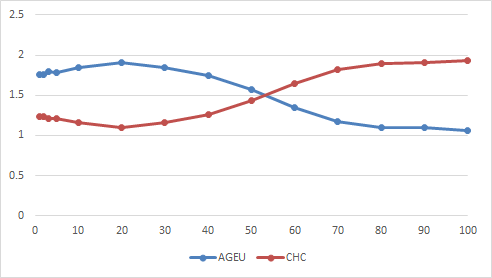
\includegraphics[scale=0.8]{imagenes/Experimental/AGEUvsCHC.png}
        \caption{Comparación de AGEU y CHC}
        \label{fig:AGEUvsCHC}
\end{figure}

También podemos apreciar en la tabla \ref{diferenciasAGEU} la media de las distancias entre las soluciones obtenidas en cada \textit{milestone} en la ejecución de AGEU con la final (también más visible en la gráfica \ref{fig:DiferenciasAGEU}). 

%Diferencias AGEU
\begin{table}[]
\begin{tabular}{|cclcclccl|}
\hline
\rowcolor[HTML]{FFFFC7} 
\multicolumn{9}{|c|}{\cellcolor[HTML]{FFFFC7}AGEU   450}                                                                                                                                                                                                                                                                                                                                                                                                                                                                     \\ \hline
\rowcolor[HTML]{FCE6AB} 
\multicolumn{1}{|c|}{\cellcolor[HTML]{FCE6AB}n}                      & \multicolumn{1}{c|}{\cellcolor[HTML]{FCE6AB}milestone} & \multicolumn{1}{l|}{\cellcolor[HTML]{FCE6AB}Diferencia} & \multicolumn{1}{c|}{\cellcolor[HTML]{FCE6AB}n}                      & \multicolumn{1}{c|}{\cellcolor[HTML]{FCE6AB}milestone} & \multicolumn{1}{l|}{\cellcolor[HTML]{FCE6AB}Diferencia} & \multicolumn{1}{c|}{\cellcolor[HTML]{FCE6AB}n}                      & \multicolumn{1}{c|}{\cellcolor[HTML]{FCE6AB}milestone} & Diferencia \\ \hline
\rowcolor[HTML]{DAE8FC} 
\multicolumn{1}{|c|}{\cellcolor[HTML]{FFFFC7}}                       & \multicolumn{1}{c|}{\cellcolor[HTML]{DAE8FC}1}         & \multicolumn{1}{l|}{\cellcolor[HTML]{DAE8FC}11066.03}   & \multicolumn{1}{c|}{\cellcolor[HTML]{FFFFC7}}                       & \multicolumn{1}{c|}{\cellcolor[HTML]{DAE8FC}1}         & \multicolumn{1}{l|}{\cellcolor[HTML]{DAE8FC}54979.9692} & \multicolumn{1}{c|}{\cellcolor[HTML]{FFFFC7}}                       & \multicolumn{1}{c|}{\cellcolor[HTML]{DAE8FC}1}         & 77065.6989 \\ \cline{2-3} \cline{5-6} \cline{8-9} 
\rowcolor[HTML]{DDFDFF} 
\multicolumn{1}{|c|}{\cellcolor[HTML]{FFFFC7}}                       & \multicolumn{1}{c|}{\cellcolor[HTML]{DDFDFF}2}         & \multicolumn{1}{l|}{\cellcolor[HTML]{DDFDFF}8843.503}   & \multicolumn{1}{c|}{\cellcolor[HTML]{FFFFC7}}                       & \multicolumn{1}{c|}{\cellcolor[HTML]{DDFDFF}2}         & \multicolumn{1}{l|}{\cellcolor[HTML]{DDFDFF}45735.6846} & \multicolumn{1}{c|}{\cellcolor[HTML]{FFFFC7}}                       & \multicolumn{1}{c|}{\cellcolor[HTML]{DDFDFF}2}         & 65917.1705 \\ \cline{2-3} \cline{5-6} \cline{8-9} 
\rowcolor[HTML]{DAE8FC} 
\multicolumn{1}{|c|}{\cellcolor[HTML]{FFFFC7}}                       & \multicolumn{1}{c|}{\cellcolor[HTML]{DAE8FC}3}         & \multicolumn{1}{l|}{\cellcolor[HTML]{DAE8FC}7640.7}     & \multicolumn{1}{c|}{\cellcolor[HTML]{FFFFC7}}                       & \multicolumn{1}{c|}{\cellcolor[HTML]{DAE8FC}3}         & \multicolumn{1}{l|}{\cellcolor[HTML]{DAE8FC}41236.5128} & \multicolumn{1}{c|}{\cellcolor[HTML]{FFFFC7}}                       & \multicolumn{1}{c|}{\cellcolor[HTML]{DAE8FC}3}         & 60357.7768 \\ \cline{2-3} \cline{5-6} \cline{8-9} 
\rowcolor[HTML]{DDFDFF} 
\multicolumn{1}{|c|}{\cellcolor[HTML]{FFFFC7}}                       & \multicolumn{1}{c|}{\cellcolor[HTML]{DDFDFF}5}         & \multicolumn{1}{l|}{\cellcolor[HTML]{DDFDFF}5932.67}    & \multicolumn{1}{c|}{\cellcolor[HTML]{FFFFC7}}                       & \multicolumn{1}{c|}{\cellcolor[HTML]{DDFDFF}5}         & \multicolumn{1}{l|}{\cellcolor[HTML]{DDFDFF}33487.7872} & \multicolumn{1}{c|}{\cellcolor[HTML]{FFFFC7}}                       & \multicolumn{1}{c|}{\cellcolor[HTML]{DDFDFF}5}         & 50938.9158 \\ \cline{2-3} \cline{5-6} \cline{8-9} 
\rowcolor[HTML]{DAE8FC} 
\multicolumn{1}{|c|}{\cellcolor[HTML]{FFFFC7}}                       & \multicolumn{1}{c|}{\cellcolor[HTML]{DAE8FC}10}        & \multicolumn{1}{l|}{\cellcolor[HTML]{DAE8FC}3436.968}   & \multicolumn{1}{c|}{\cellcolor[HTML]{FFFFC7}}                       & \multicolumn{1}{c|}{\cellcolor[HTML]{DAE8FC}10}        & \multicolumn{1}{l|}{\cellcolor[HTML]{DAE8FC}22116.0077} & \multicolumn{1}{c|}{\cellcolor[HTML]{FFFFC7}}                       & \multicolumn{1}{c|}{\cellcolor[HTML]{DAE8FC}10}        & 36641.6095 \\ \cline{2-3} \cline{5-6} \cline{8-9} 
\rowcolor[HTML]{DDFDFF} 
\multicolumn{1}{|c|}{\cellcolor[HTML]{FFFFC7}}                       & \multicolumn{1}{c|}{\cellcolor[HTML]{DDFDFF}20}        & \multicolumn{1}{l|}{\cellcolor[HTML]{DDFDFF}1524.318}   & \multicolumn{1}{c|}{\cellcolor[HTML]{FFFFC7}}                       & \multicolumn{1}{c|}{\cellcolor[HTML]{DDFDFF}20}        & \multicolumn{1}{l|}{\cellcolor[HTML]{DDFDFF}11864.6333} & \multicolumn{1}{c|}{\cellcolor[HTML]{FFFFC7}}                       & \multicolumn{1}{c|}{\cellcolor[HTML]{DDFDFF}20}        & 23155.9916 \\ \cline{2-3} \cline{5-6} \cline{8-9} 
\rowcolor[HTML]{DAE8FC} 
\multicolumn{1}{|c|}{\cellcolor[HTML]{FFFFC7}}                       & \multicolumn{1}{c|}{\cellcolor[HTML]{DAE8FC}30}        & \multicolumn{1}{l|}{\cellcolor[HTML]{DAE8FC}785.4641}   & \multicolumn{1}{c|}{\cellcolor[HTML]{FFFFC7}}                       & \multicolumn{1}{c|}{\cellcolor[HTML]{DAE8FC}30}        & \multicolumn{1}{l|}{\cellcolor[HTML]{DAE8FC}7146.58462} & \multicolumn{1}{c|}{\cellcolor[HTML]{FFFFC7}}                       & \multicolumn{1}{c|}{\cellcolor[HTML]{DAE8FC}30}        & 16188.8274 \\ \cline{2-3} \cline{5-6} \cline{8-9} 
\rowcolor[HTML]{DDFDFF} 
\multicolumn{1}{|c|}{\cellcolor[HTML]{FFFFC7}}                       & \multicolumn{1}{c|}{\cellcolor[HTML]{DDFDFF}40}        & \multicolumn{1}{l|}{\cellcolor[HTML]{DDFDFF}450.1636}   & \multicolumn{1}{c|}{\cellcolor[HTML]{FFFFC7}}                       & \multicolumn{1}{c|}{\cellcolor[HTML]{DDFDFF}40}        & \multicolumn{1}{l|}{\cellcolor[HTML]{DDFDFF}4390.63846} & \multicolumn{1}{c|}{\cellcolor[HTML]{FFFFC7}}                       & \multicolumn{1}{c|}{\cellcolor[HTML]{DDFDFF}40}        & 11630.5558 \\ \cline{2-3} \cline{5-6} \cline{8-9} 
\rowcolor[HTML]{DAE8FC} 
\multicolumn{1}{|c|}{\cellcolor[HTML]{FFFFC7}}                       & \multicolumn{1}{c|}{\cellcolor[HTML]{DAE8FC}50}        & \multicolumn{1}{l|}{\cellcolor[HTML]{DAE8FC}260.5513}   & \multicolumn{1}{c|}{\cellcolor[HTML]{FFFFC7}}                       & \multicolumn{1}{c|}{\cellcolor[HTML]{DAE8FC}50}        & \multicolumn{1}{l|}{\cellcolor[HTML]{DAE8FC}2667.21538} & \multicolumn{1}{c|}{\cellcolor[HTML]{FFFFC7}}                       & \multicolumn{1}{c|}{\cellcolor[HTML]{DAE8FC}50}        & 8142.90526 \\ \cline{2-3} \cline{5-6} \cline{8-9} 
\rowcolor[HTML]{DDFDFF} 
\multicolumn{1}{|c|}{\cellcolor[HTML]{FFFFC7}}                       & \multicolumn{1}{c|}{\cellcolor[HTML]{DDFDFF}60}        & \multicolumn{1}{l|}{\cellcolor[HTML]{DDFDFF}156.6538}   & \multicolumn{1}{c|}{\cellcolor[HTML]{FFFFC7}}                       & \multicolumn{1}{c|}{\cellcolor[HTML]{DDFDFF}60}        & \multicolumn{1}{l|}{\cellcolor[HTML]{DDFDFF}1570.27692} & \multicolumn{1}{c|}{\cellcolor[HTML]{FFFFC7}}                       & \multicolumn{1}{c|}{\cellcolor[HTML]{DDFDFF}60}        & 5593.12105 \\ \cline{2-3} \cline{5-6} \cline{8-9} 
\rowcolor[HTML]{DAE8FC} 
\multicolumn{1}{|c|}{\cellcolor[HTML]{FFFFC7}}                       & \multicolumn{1}{c|}{\cellcolor[HTML]{DAE8FC}70}        & \multicolumn{1}{l|}{\cellcolor[HTML]{DAE8FC}90.98718}   & \multicolumn{1}{c|}{\cellcolor[HTML]{FFFFC7}}                       & \multicolumn{1}{c|}{\cellcolor[HTML]{DAE8FC}70}        & \multicolumn{1}{l|}{\cellcolor[HTML]{DAE8FC}952.261538} & \multicolumn{1}{c|}{\cellcolor[HTML]{FFFFC7}}                       & \multicolumn{1}{c|}{\cellcolor[HTML]{DAE8FC}70}        & 3610.04316 \\ \cline{2-3} \cline{5-6} \cline{8-9} 
\rowcolor[HTML]{DDFDFF} 
\multicolumn{1}{|c|}{\cellcolor[HTML]{FFFFC7}}                       & \multicolumn{1}{c|}{\cellcolor[HTML]{DDFDFF}80}        & \multicolumn{1}{l|}{\cellcolor[HTML]{DDFDFF}54.53077}   & \multicolumn{1}{c|}{\cellcolor[HTML]{FFFFC7}}                       & \multicolumn{1}{c|}{\cellcolor[HTML]{DDFDFF}80}        & \multicolumn{1}{l|}{\cellcolor[HTML]{DDFDFF}525.023077} & \multicolumn{1}{c|}{\cellcolor[HTML]{FFFFC7}}                       & \multicolumn{1}{c|}{\cellcolor[HTML]{DDFDFF}80}        & 2010.8     \\ \cline{2-3} \cline{5-6} \cline{8-9} 
\rowcolor[HTML]{DAE8FC} 
\multicolumn{1}{|c|}{\multirow{-13}{*}{\cellcolor[HTML]{FFFFC7}100}} & \multicolumn{1}{c|}{\cellcolor[HTML]{DAE8FC}90}        & \multicolumn{1}{l|}{\cellcolor[HTML]{DAE8FC}26.47692}   & \multicolumn{1}{c|}{\multirow{-13}{*}{\cellcolor[HTML]{FFFFC7}200}} & \multicolumn{1}{c|}{\cellcolor[HTML]{DAE8FC}90}        & \multicolumn{1}{l|}{\cellcolor[HTML]{DAE8FC}201.676923} & \multicolumn{1}{c|}{\multirow{-13}{*}{\cellcolor[HTML]{FFFFC7}300}} & \multicolumn{1}{c|}{\cellcolor[HTML]{DAE8FC}90}        & 855.950526 \\ \hline
\end{tabular}
\caption{\label{diferenciasAGEU}Diferencias de los resultados de las distintas milestones con respecto a la final para el AG}
\end{table}

\begin{figure}
		\centering
		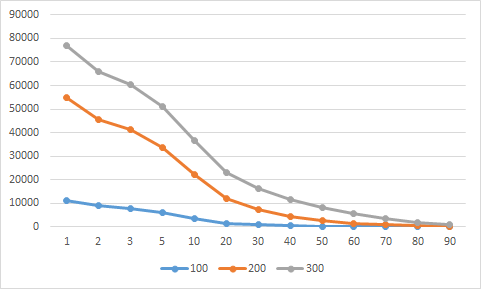
\includegraphics[scale=1]{imagenes/Experimental/DiferenciasAGEU.png}
        \caption{Gráfica asociada a la tabla \ref{diferenciasAGEU}}
        \label{fig:DiferenciasAGEU}
\end{figure}

De la misma forma, en la tabla \ref{DiferenciasCHC} se puede apreciar la media de las diferencias entre las soluciones obtenidas en cada \textit{milestone} de la ejecución del algoritmo CHC con la final (también más visible en la gráfica \ref{fig:DiferenciasCHC}). 

\begin{table}[h]
\begin{tabular}{|cclcclccl|}
\hline
\rowcolor[HTML]{FFFFC7} 
\multicolumn{9}{|c|}{\cellcolor[HTML]{FFFFC7}CHC   450}                                                                                                                                                                                                                                                                                                                                                                                                                                                                                                 \\ \hline
\rowcolor[HTML]{F7EAC7} 
\multicolumn{1}{|c|}{\cellcolor[HTML]{F7EAC7}n}                               & \multicolumn{1}{c|}{\cellcolor[HTML]{F7EAC7}milestone} & \multicolumn{1}{l|}{\cellcolor[HTML]{F7EAC7}Diferencia} & \multicolumn{1}{c|}{\cellcolor[HTML]{F7EAC7}n}                               & \multicolumn{1}{c|}{\cellcolor[HTML]{F7EAC7}milestone} & \multicolumn{1}{l|}{\cellcolor[HTML]{F7EAC7}Diferencia} & \multicolumn{1}{c|}{\cellcolor[HTML]{F7EAC7}n}                               & \multicolumn{1}{c|}{\cellcolor[HTML]{F7EAC7}milestone} & Diferencia \\ \hline
\rowcolor[HTML]{DAE8FC} 
\multicolumn{1}{|c|}{\cellcolor[HTML]{FFFFC7}}                                & \multicolumn{1}{c|}{\cellcolor[HTML]{DAE8FC}1}         & \multicolumn{1}{l|}{\cellcolor[HTML]{DAE8FC}5550.43}    & \multicolumn{1}{c|}{\cellcolor[HTML]{FFFFC7}}                                & \multicolumn{1}{c|}{\cellcolor[HTML]{DAE8FC}1}         & \multicolumn{1}{l|}{\cellcolor[HTML]{DAE8FC}30637.1928} & \multicolumn{1}{c|}{\cellcolor[HTML]{FFFFC7}}                                & \multicolumn{1}{c|}{\cellcolor[HTML]{DAE8FC}1}         & 45581.5337 \\ \cline{2-3} \cline{5-6} \cline{8-9} 
\rowcolor[HTML]{DDFDFF} 
\multicolumn{1}{|c|}{\cellcolor[HTML]{FFFFC7}}                                & \multicolumn{1}{c|}{\cellcolor[HTML]{DDFDFF}2}         & \multicolumn{1}{l|}{\cellcolor[HTML]{DDFDFF}4274.04}    & \multicolumn{1}{c|}{\cellcolor[HTML]{FFFFC7}}                                & \multicolumn{1}{c|}{\cellcolor[HTML]{DDFDFF}2}         & \multicolumn{1}{l|}{\cellcolor[HTML]{DDFDFF}25432.9928} & \multicolumn{1}{c|}{\cellcolor[HTML]{FFFFC7}}                                & \multicolumn{1}{c|}{\cellcolor[HTML]{DDFDFF}2}         & 38276.1389 \\ \cline{2-3} \cline{5-6} \cline{8-9} 
\rowcolor[HTML]{DAE8FC} 
\multicolumn{1}{|c|}{\cellcolor[HTML]{FFFFC7}}                                & \multicolumn{1}{c|}{\cellcolor[HTML]{DAE8FC}3}         & \multicolumn{1}{l|}{\cellcolor[HTML]{DAE8FC}3519.52}    & \multicolumn{1}{c|}{\cellcolor[HTML]{FFFFC7}}                                & \multicolumn{1}{c|}{\cellcolor[HTML]{DAE8FC}3}         & \multicolumn{1}{l|}{\cellcolor[HTML]{DAE8FC}23040.4954} & \multicolumn{1}{c|}{\cellcolor[HTML]{FFFFC7}}                                & \multicolumn{1}{c|}{\cellcolor[HTML]{DAE8FC}3}         & 35398.4705 \\ \cline{2-3} \cline{5-6} \cline{8-9} 
\rowcolor[HTML]{DDFDFF} 
\multicolumn{1}{|c|}{\cellcolor[HTML]{FFFFC7}}                                & \multicolumn{1}{c|}{\cellcolor[HTML]{DDFDFF}5}         & \multicolumn{1}{l|}{\cellcolor[HTML]{DDFDFF}2291.48}    & \multicolumn{1}{c|}{\cellcolor[HTML]{FFFFC7}}                                & \multicolumn{1}{c|}{\cellcolor[HTML]{DDFDFF}5}         & \multicolumn{1}{l|}{\cellcolor[HTML]{DDFDFF}19181.1441} & \multicolumn{1}{c|}{\cellcolor[HTML]{FFFFC7}}                                & \multicolumn{1}{c|}{\cellcolor[HTML]{DDFDFF}5}         & 30803.3284 \\ \cline{2-3} \cline{5-6} \cline{8-9} 
\rowcolor[HTML]{DAE8FC} 
\multicolumn{1}{|c|}{\cellcolor[HTML]{FFFFC7}}                                & \multicolumn{1}{c|}{\cellcolor[HTML]{DAE8FC}10}        & \multicolumn{1}{l|}{\cellcolor[HTML]{DAE8FC}401.851}    & \multicolumn{1}{c|}{\cellcolor[HTML]{FFFFC7}}                                & \multicolumn{1}{c|}{\cellcolor[HTML]{DAE8FC}10}        & \multicolumn{1}{l|}{\cellcolor[HTML]{DAE8FC}9927.18205} & \multicolumn{1}{c|}{\cellcolor[HTML]{FFFFC7}}                                & \multicolumn{1}{c|}{\cellcolor[HTML]{DAE8FC}10}        & 21616.4158 \\ \cline{2-3} \cline{5-6} \cline{8-9} 
\rowcolor[HTML]{DDFDFF} 
\multicolumn{1}{|c|}{\cellcolor[HTML]{FFFFC7}}                                & \multicolumn{1}{c|}{\cellcolor[HTML]{DDFDFF}20}        & \multicolumn{1}{l|}{\cellcolor[HTML]{DDFDFF}1.56154}    & \multicolumn{1}{c|}{\cellcolor[HTML]{FFFFC7}}                                & \multicolumn{1}{c|}{\cellcolor[HTML]{DDFDFF}20}        & \multicolumn{1}{l|}{\cellcolor[HTML]{DDFDFF}828.928205} & \multicolumn{1}{c|}{\cellcolor[HTML]{FFFFC7}}                                & \multicolumn{1}{c|}{\cellcolor[HTML]{DDFDFF}20}        & 7160.64737 \\ \cline{2-3} \cline{5-6} \cline{8-9} 
\rowcolor[HTML]{DAE8FC} 
\multicolumn{1}{|c|}{\cellcolor[HTML]{FFFFC7}}                                & \multicolumn{1}{c|}{\cellcolor[HTML]{DAE8FC}30}        & \multicolumn{1}{l|}{\cellcolor[HTML]{DAE8FC}0.02564}    & \multicolumn{1}{c|}{\cellcolor[HTML]{FFFFC7}}                                & \multicolumn{1}{c|}{\cellcolor[HTML]{DAE8FC}30}        & \multicolumn{1}{l|}{\cellcolor[HTML]{DAE8FC}7.98717949} & \multicolumn{1}{c|}{\cellcolor[HTML]{FFFFC7}}                                & \multicolumn{1}{c|}{\cellcolor[HTML]{DAE8FC}30}        & 688.815789 \\ \cline{2-3} \cline{5-6} \cline{8-9} 
\rowcolor[HTML]{DDFDFF} 
\multicolumn{1}{|c|}{\cellcolor[HTML]{FFFFC7}}                                & \multicolumn{1}{c|}{\cellcolor[HTML]{DDFDFF}40}        & \multicolumn{1}{l|}{\cellcolor[HTML]{DDFDFF}0}          & \multicolumn{1}{c|}{\cellcolor[HTML]{FFFFC7}}                                & \multicolumn{1}{c|}{\cellcolor[HTML]{DDFDFF}40}        & \multicolumn{1}{l|}{\cellcolor[HTML]{DDFDFF}0.69230769} & \multicolumn{1}{c|}{\cellcolor[HTML]{FFFFC7}}                                & \multicolumn{1}{c|}{\cellcolor[HTML]{DDFDFF}40}        & 8.42105263 \\ \cline{2-3} \cline{5-6} \cline{8-9} 
\rowcolor[HTML]{DAE8FC} 
\multicolumn{1}{|c|}{\cellcolor[HTML]{FFFFC7}}                                & \multicolumn{1}{c|}{\cellcolor[HTML]{DAE8FC}50}        & \multicolumn{1}{l|}{\cellcolor[HTML]{DAE8FC}0}          & \multicolumn{1}{c|}{\cellcolor[HTML]{FFFFC7}}                                & \multicolumn{1}{c|}{\cellcolor[HTML]{DAE8FC}50}        & \multicolumn{1}{l|}{\cellcolor[HTML]{DAE8FC}0.17948718} & \multicolumn{1}{c|}{\cellcolor[HTML]{FFFFC7}}                                & \multicolumn{1}{c|}{\cellcolor[HTML]{DAE8FC}50}        & 0.47368421 \\ \cline{2-3} \cline{5-6} \cline{8-9} 
\rowcolor[HTML]{DDFDFF} 
\multicolumn{1}{|c|}{\cellcolor[HTML]{FFFFC7}}                                & \multicolumn{1}{c|}{\cellcolor[HTML]{DDFDFF}60}        & \multicolumn{1}{l|}{\cellcolor[HTML]{DDFDFF}0}          & \multicolumn{1}{c|}{\cellcolor[HTML]{FFFFC7}}                                & \multicolumn{1}{c|}{\cellcolor[HTML]{DDFDFF}60}        & \multicolumn{1}{l|}{\cellcolor[HTML]{DDFDFF}0}          & \multicolumn{1}{c|}{\cellcolor[HTML]{FFFFC7}}                                & \multicolumn{1}{c|}{\cellcolor[HTML]{DDFDFF}60}        & 0          \\ \cline{2-3} \cline{5-6} \cline{8-9} 
\rowcolor[HTML]{DAE8FC} 
\multicolumn{1}{|c|}{\cellcolor[HTML]{FFFFC7}}                                & \multicolumn{1}{c|}{\cellcolor[HTML]{DAE8FC}70}        & \multicolumn{1}{l|}{\cellcolor[HTML]{DAE8FC}0}          & \multicolumn{1}{c|}{\cellcolor[HTML]{FFFFC7}}                                & \multicolumn{1}{c|}{\cellcolor[HTML]{DAE8FC}70}        & \multicolumn{1}{l|}{\cellcolor[HTML]{DAE8FC}0}          & \multicolumn{1}{c|}{\cellcolor[HTML]{FFFFC7}}                                & \multicolumn{1}{c|}{\cellcolor[HTML]{DAE8FC}70}        & 0          \\ \cline{2-3} \cline{5-6} \cline{8-9} 
\rowcolor[HTML]{DDFDFF} 
\multicolumn{1}{|c|}{\cellcolor[HTML]{FFFFC7}}                                & \multicolumn{1}{c|}{\cellcolor[HTML]{DDFDFF}80}        & \multicolumn{1}{l|}{\cellcolor[HTML]{DDFDFF}0}          & \multicolumn{1}{c|}{\cellcolor[HTML]{FFFFC7}}                                & \multicolumn{1}{c|}{\cellcolor[HTML]{DDFDFF}80}        & \multicolumn{1}{l|}{\cellcolor[HTML]{DDFDFF}0}          & \multicolumn{1}{c|}{\cellcolor[HTML]{FFFFC7}}                                & \multicolumn{1}{c|}{\cellcolor[HTML]{DDFDFF}80}        & 0          \\ \cline{2-3} \cline{5-6} \cline{8-9} 
\rowcolor[HTML]{DAE8FC} 
\multicolumn{1}{|c|}{\multirow{-13}{*}{\cellcolor[HTML]{FFFFC7}\textbf{100}}} & \multicolumn{1}{c|}{\cellcolor[HTML]{DAE8FC}90}        & \multicolumn{1}{l|}{\cellcolor[HTML]{DAE8FC}0}          & \multicolumn{1}{c|}{\multirow{-13}{*}{\cellcolor[HTML]{FFFFC7}\textbf{200}}} & \multicolumn{1}{c|}{\cellcolor[HTML]{DAE8FC}90}        & \multicolumn{1}{l|}{\cellcolor[HTML]{DAE8FC}0}          & \multicolumn{1}{c|}{\multirow{-13}{*}{\cellcolor[HTML]{FFFFC7}\textbf{300}}} & \multicolumn{1}{c|}{\cellcolor[HTML]{DAE8FC}90}        & 0          \\ \hline
\end{tabular}
\caption{\label{DiferenciasCHC}Diferencias de los resultados de las distintas milestones con respecto a la final para el algoritmo CHC}
\end{table}

\begin{figure}[h]
		\centering
		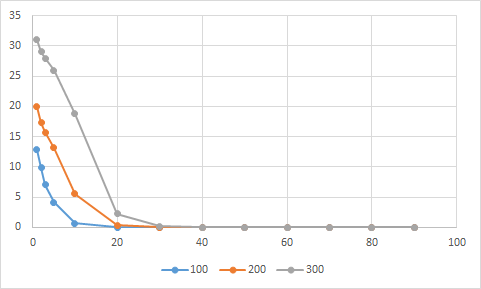
\includegraphics[scale=1]{imagenes/Experimental/DiferenciasCHC.png}
        \caption{Gráfica asociada a la tabla \ref{DiferenciasCHC}}
        \label{fig:DiferenciasCHC}
\end{figure}

Por lo que se puede ver en la tabla \ref{diferenciasAGEU} no se puede decir que converja prematuramente, de hecho en todo momento realiza mejoras significativas. 
Esto se puede observar en el hecho de que las diferencias a la última solución van disminuyendo en gran medida en cada una de las \textit{milestones}. 

Sin embargo, en la tabla \ref{DiferenciasCHC} se tiene que las soluciones convergen rápidamente a la solución final antes de llegar siquiera el 50\% de la ejecución total. 
De esto se puede inferir que los mecanismos de aumento de la diversidad de CHC no son de mucha utilidad en nuestro caso. 

Por otra parte, si nos fijamos en la gráfica \ref{fig:AGEUvsCHC} se puede ver cómo el algoritmo CHC es mejor que el AGEU mientras que se siguen produciendo cambios, es decir, antes de que se produzca el 50\% de la ejecución. 
Por lo que se considerará posteriormente una mezcla de ambos algoritmos, con el fin de aprovechar los buenos resultados iniciales del CHC y la capacidad de no converger rápidamente que presenta AGEU con el fin de tener un buen punto de partida.

\section{Incorporación del histórico}

La primera modificación que se propone es la introducción de un histórico, explicado en la primera sección del capítulo anterior. 
La principal motivación de esta modificación es incidir en la explotación de las buenas soluciones, ya que se almacenarán los elementos más predominantes en las mejores soluciones y en las peores, con el fin de reincidir con mayor frecuencia en los primeros y rehuir de los segundos. 

Obviamente, este histórico deberá tener un proceso de aprendizaje (en el que almacena todas las soluciones distintas para luego discernir cuáles son las mejores y cuáles las peores y sus respectivos elementos) y un proceso de reacción, en la que pondrá en práctica la información aprendida en la fase anterior. 
Con el fin de que no sea un único procedimiento y pueda ir aprendiendo a lo largo de la ejecución (para intentar evitar quedarse en máximos locales), estas dos fases se irán turnando cada 50 generaciones. 

Para poner a prueba su utilidad, se estudian los resultados obtenidos de aplicar el histórico solo al operador de reparación (si tiene que añadir elementos, elegirá los mejores; si tiene que eliminar elementos, elegirá los peores), solo a la mutación (tiene prioridad insertar mejores elementos y eliminar peores) y a ambos a la vez. 
Los resultados de este estudio se muestran en la tabla (apéndice?) y, más visualmente, en la gráfica \ref{fig:Historico}.

\begin{figure}[h]
		\centering
		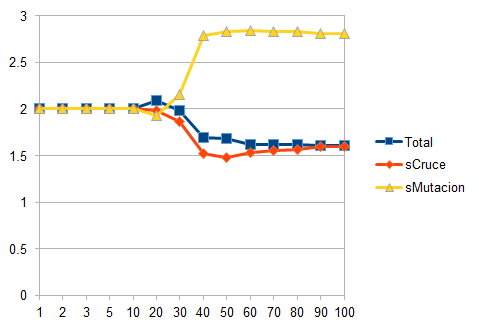
\includegraphics[scale=1]{imagenes/Experimental/Historico.png}
        \caption{Resultados de aplicar el histórico}
        \label{fig:Historico}
\end{figure}

En esta gráfica \ref{fig:Historico} podemos apreciar que las mejores opciones son aplicarlo solo al cruce o a ambos; de hecho, por muy pocas milésimas se tiene que solo aplicarlo al cruce es mejor, pero es una diferencia tan insignificante que se ha decidido continuar con la aplicación del histórico a ambos, para mantener la consistencia, y porque es posible que en algún momento del desarrollo se puedan realizar más modificaciones a la mutación de las que el histórico se podría aprovechar. 

Además, que cuando solo se aplique el histórico a la mutación de los peores resultados con diferencia es una primera indicación de que la introducción del histórico ha supuesto una mejora al modelo original.
Esto se debe a que realmente la mutación se produce un número muy bajo de veces y no suele producir grandes cambios, por lo que si es lo único que se modifica, es muy probable que no se distancie mucho de los resultados originales. 
Para confirmar esta idea y poder asegurarnos de que se ha dado un paso en una dirección correcta, comparamos en la gráfica \ref{fig:AGEUvsGACEP} los resultados originales y los de aplicar el histórico a ambos operadores. 

\begin{figure}[h]
		\centering
		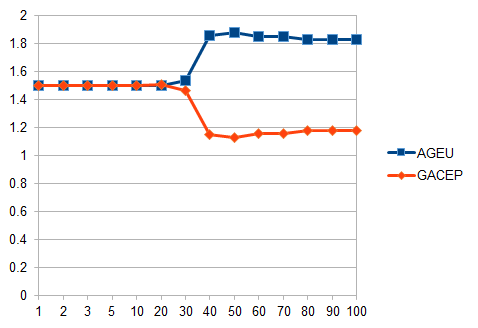
\includegraphics[scale=1]{imagenes/Experimental/AGEUvsGACEP.png}
        \caption{Comparación de los resultados del AGEU y la aplicación del histórico}
        \label{fig:AGEUvsGACEP}
\end{figure}

Con esta gráfica \ref{fig:AGEUvsGACEP} quedan confirmadas nuestras suposiciones. 
Es importante mencionar que en sus primeras iteraciones ambos algoritmos obtienen los mismos resultados ya que se comportan de la misma forma. 
Recordemos que cada fase del histórico ocupa 50 iteraciones, por lo que durante las primeras 50 iteraciones va a mantener el mismo comportamiento que AGEU, con la excepción de que va a ir almacenando las soluciones para su posterior análisis. 
Estas 50 iteraciones suponen un poco más del 10\% inicial de las iteraciones totales, por lo que es obvio que para todas estas \textit{milestones} sus resultados van a ser iguales. 
También cabe la pena mencionar que en el momento en el que difieren los resultados de los algoritmos, su clasificación se mantiene casi constante, por lo que queda claro que el uso del histórico hace que el algoritmo sea consistentemente mejor.  

Es más, con esta modificación podemos crear las bases de lo que será nuestro nuevo algoritmo, al cual llamaremos \textbf{GACEP} (\textbf{\textit{Genetic Algorithm for Combinatory Expensive Problem}}). 

Los resultados de la ejecución de este algoritmo vienen recopilados en la tabla \ref{GACEP_Historico}.

% Please add the following required packages to your document preamble:
% \usepackage{multirow}
% \usepackage[table,xcdraw]{xcolor}
% If you use beamer only pass "xcolor=table" option, i.e. \documentclass[xcolor=table]{beamer}
\begin{table}[]
\begin{tabular}{|cclccllll}
\hline
\rowcolor[HTML]{FFFFC7} 
\multicolumn{9}{|c|}{\cellcolor[HTML]{FFFFC7}GACEP}                                                                                                                                                                                                                                                                                                                                                                                                                                                                                                                                                                                    \\ \hline
\rowcolor[HTML]{F7EAC7} 
\multicolumn{1}{|c|}{\cellcolor[HTML]{F7EAC7}n}                               & \multicolumn{1}{c|}{\cellcolor[HTML]{F7EAC7}densidad}              & \multicolumn{1}{c|}{\cellcolor[HTML]{F7EAC7}Resultado} & \multicolumn{1}{c|}{\cellcolor[HTML]{F7EAC7}n}                               & \multicolumn{1}{c|}{\cellcolor[HTML]{F7EAC7}densidad}               & \multicolumn{1}{c|}{\cellcolor[HTML]{F7EAC7}Resultado} & \multicolumn{1}{c|}{\cellcolor[HTML]{F7EAC7}n}                               & \multicolumn{1}{c|}{\cellcolor[HTML]{F7EAC7}densidad}              & \multicolumn{1}{c|}{\cellcolor[HTML]{F7EAC7}Resultado} \\ \hline
\rowcolor[HTML]{DAE8FC} 
\multicolumn{1}{|c|}{\cellcolor[HTML]{FFFFC7}}                                & \multicolumn{1}{c|}{\cellcolor[HTML]{DAE8FC}}                      & \multicolumn{1}{l|}{\cellcolor[HTML]{DAE8FC}203917}    & \multicolumn{1}{c|}{\cellcolor[HTML]{FFFFC7}}                                & \multicolumn{1}{c|}{\cellcolor[HTML]{DAE8FC}}                       & \multicolumn{1}{l|}{\cellcolor[HTML]{DAE8FC}371906}    & \multicolumn{1}{c|}{\cellcolor[HTML]{FFFFC7}}                                & \multicolumn{1}{c|}{\cellcolor[HTML]{DAE8FC}}                      & \multicolumn{1}{l|}{\cellcolor[HTML]{DAE8FC}370202}    \\ \cline{3-3} \cline{6-6} \cline{9-9} 
\multicolumn{1}{|c|}{\cellcolor[HTML]{FFFFC7}}                                & \multicolumn{1}{c|}{\cellcolor[HTML]{DAE8FC}}                      & \multicolumn{1}{l|}{\cellcolor[HTML]{DDFDFF}86893.8}   & \multicolumn{1}{c|}{\cellcolor[HTML]{FFFFC7}}                                & \multicolumn{1}{c|}{\cellcolor[HTML]{DAE8FC}}                       & \multicolumn{1}{l|}{\cellcolor[HTML]{DDFDFF}960695}    & \multicolumn{1}{c|}{\cellcolor[HTML]{FFFFC7}}                                & \multicolumn{1}{c|}{\cellcolor[HTML]{DAE8FC}}                      & \multicolumn{1}{l|}{\cellcolor[HTML]{DDFDFF}30668.8}   \\ \cline{3-3} \cline{6-6} \cline{9-9} 
\rowcolor[HTML]{DAE8FC} 
\multicolumn{1}{|c|}{\cellcolor[HTML]{FFFFC7}}                                & \multicolumn{1}{c|}{\cellcolor[HTML]{DAE8FC}}                      & \multicolumn{1}{l|}{\cellcolor[HTML]{DAE8FC}202056}    & \multicolumn{1}{c|}{\cellcolor[HTML]{FFFFC7}}                                & \multicolumn{1}{c|}{\cellcolor[HTML]{DAE8FC}}                       & \multicolumn{1}{l|}{\cellcolor[HTML]{DAE8FC}310368}    & \multicolumn{1}{c|}{\cellcolor[HTML]{FFFFC7}}                                & \multicolumn{1}{c|}{\cellcolor[HTML]{DAE8FC}}                      & \multicolumn{1}{l|}{\cellcolor[HTML]{DAE8FC}261697}    \\ \cline{3-3} \cline{6-6} \cline{9-9} 
\multicolumn{1}{|c|}{\cellcolor[HTML]{FFFFC7}}                                & \multicolumn{1}{c|}{\cellcolor[HTML]{DAE8FC}}                      & \multicolumn{1}{l|}{\cellcolor[HTML]{DDFDFF}234528}    & \multicolumn{1}{c|}{\cellcolor[HTML]{FFFFC7}}                                & \multicolumn{1}{c|}{\cellcolor[HTML]{DAE8FC}}                       & \multicolumn{1}{l|}{\cellcolor[HTML]{DDFDFF}31956}     & \multicolumn{1}{c|}{\cellcolor[HTML]{FFFFC7}}                                & \multicolumn{1}{c|}{\cellcolor[HTML]{DAE8FC}}                      & \multicolumn{1}{l|}{\cellcolor[HTML]{DDFDFF}441509}    \\ \cline{3-3} \cline{6-6} \cline{9-9} 
\rowcolor[HTML]{DAE8FC} 
\multicolumn{1}{|c|}{\cellcolor[HTML]{FFFFC7}}                                & \multicolumn{1}{c|}{\cellcolor[HTML]{DAE8FC}}                      & \multicolumn{1}{l|}{\cellcolor[HTML]{DAE8FC}238931}    & \multicolumn{1}{c|}{\cellcolor[HTML]{FFFFC7}}                                & \multicolumn{1}{c|}{\cellcolor[HTML]{DAE8FC}}                       & \multicolumn{1}{l|}{\cellcolor[HTML]{DAE8FC}107874}    & \multicolumn{1}{c|}{\cellcolor[HTML]{FFFFC7}}                                & \multicolumn{1}{c|}{\cellcolor[HTML]{DAE8FC}}                      & \multicolumn{1}{l|}{\cellcolor[HTML]{DAE8FC}15628.8}   \\ \cline{3-3} \cline{6-6} \cline{9-9} 
\multicolumn{1}{|c|}{\cellcolor[HTML]{FFFFC7}}                                & \multicolumn{1}{c|}{\cellcolor[HTML]{DAE8FC}}                      & \multicolumn{1}{l|}{\cellcolor[HTML]{DDFDFF}78698.4}   & \multicolumn{1}{c|}{\cellcolor[HTML]{FFFFC7}}                                & \multicolumn{1}{c|}{\cellcolor[HTML]{DAE8FC}}                       & \multicolumn{1}{l|}{\cellcolor[HTML]{DDFDFF}804278}    & \multicolumn{1}{c|}{\cellcolor[HTML]{FFFFC7}}                                & \multicolumn{1}{c|}{\cellcolor[HTML]{DAE8FC}}                      & \multicolumn{1}{l|}{\cellcolor[HTML]{DDFDFF}245342}    \\ \cline{3-3} \cline{6-6} \cline{9-9} 
\rowcolor[HTML]{DAE8FC} 
\multicolumn{1}{|c|}{\cellcolor[HTML]{FFFFC7}}                                & \multicolumn{1}{c|}{\cellcolor[HTML]{DAE8FC}}                      & \multicolumn{1}{l|}{\cellcolor[HTML]{DAE8FC}10611.2}   & \multicolumn{1}{c|}{\cellcolor[HTML]{FFFFC7}}                                & \multicolumn{1}{c|}{\cellcolor[HTML]{DAE8FC}}                       & \multicolumn{1}{l|}{\cellcolor[HTML]{DAE8FC}43930.7}   & \multicolumn{1}{c|}{\cellcolor[HTML]{FFFFC7}}                                & \multicolumn{1}{c|}{\cellcolor[HTML]{DAE8FC}}                      & \multicolumn{1}{l|}{\cellcolor[HTML]{DAE8FC}487566}    \\ \cline{3-3} \cline{6-6} \cline{9-9} 
\multicolumn{1}{|c|}{\cellcolor[HTML]{FFFFC7}}                                & \multicolumn{1}{c|}{\cellcolor[HTML]{DAE8FC}}                      & \multicolumn{1}{l|}{\cellcolor[HTML]{DDFDFF}67007.1}   & \multicolumn{1}{c|}{\cellcolor[HTML]{FFFFC7}}                                & \multicolumn{1}{c|}{\cellcolor[HTML]{DAE8FC}}                       & \multicolumn{1}{l|}{\cellcolor[HTML]{DDFDFF}711466}    & \multicolumn{1}{c|}{\cellcolor[HTML]{FFFFC7}}                                & \multicolumn{1}{c|}{\cellcolor[HTML]{DAE8FC}}                      & \multicolumn{1}{l|}{\cellcolor[HTML]{DDFDFF}9749.8}    \\ \cline{3-3} \cline{6-6} \cline{9-9} 
\rowcolor[HTML]{DAE8FC} 
\multicolumn{1}{|c|}{\cellcolor[HTML]{FFFFC7}}                                & \multicolumn{1}{c|}{\cellcolor[HTML]{DAE8FC}}                      & \multicolumn{1}{l|}{\cellcolor[HTML]{DAE8FC}241977}    & \multicolumn{1}{c|}{\cellcolor[HTML]{FFFFC7}}                                & \multicolumn{1}{c|}{\multirow{-9}{*}{\cellcolor[HTML]{DAE8FC}25}}   & \multicolumn{1}{l|}{\cellcolor[HTML]{DAE8FC}805644}    & \multicolumn{1}{c|}{\cellcolor[HTML]{FFFFC7}}                                & \multicolumn{1}{c|}{\multirow{-9}{*}{\cellcolor[HTML]{DAE8FC}25}}  & \multicolumn{1}{l|}{\cellcolor[HTML]{DAE8FC}226145}    \\ \cline{3-3} \cline{5-6} \cline{8-9} 
\multicolumn{1}{|c|}{\cellcolor[HTML]{FFFFC7}}                                & \multicolumn{1}{c|}{\multirow{-10}{*}{\cellcolor[HTML]{DAE8FC}25}} & \multicolumn{1}{l|}{\cellcolor[HTML]{DDFDFF}26107.5}   & \multicolumn{1}{c|}{\cellcolor[HTML]{FFFFC7}}                                & \multicolumn{1}{c|}{\cellcolor[HTML]{DDFDFF}}                       & \multicolumn{1}{l|}{\cellcolor[HTML]{DAE8FC}639675}    & \multicolumn{1}{c|}{\cellcolor[HTML]{FFFFC7}}                                & \multicolumn{1}{c|}{\cellcolor[HTML]{DDFDFF}}                      & \multicolumn{1}{l|}{\cellcolor[HTML]{DAE8FC}1009100}   \\ \cline{2-3} \cline{6-6} \cline{9-9} 
\rowcolor[HTML]{DDFDFF} 
\multicolumn{1}{|c|}{\cellcolor[HTML]{FFFFC7}}                                & \multicolumn{1}{c|}{\cellcolor[HTML]{DDFDFF}}                      & \multicolumn{1}{l|}{\cellcolor[HTML]{DAE8FC}20195.7}   & \multicolumn{1}{c|}{\cellcolor[HTML]{FFFFC7}}                                & \multicolumn{1}{c|}{\cellcolor[HTML]{DDFDFF}}                       & \multicolumn{1}{l|}{\cellcolor[HTML]{DDFDFF}49255.1}   & \multicolumn{1}{c|}{\cellcolor[HTML]{FFFFC7}}                                & \multicolumn{1}{c|}{\cellcolor[HTML]{DDFDFF}}                      & \multicolumn{1}{l|}{\cellcolor[HTML]{DDFDFF}469319}    \\ \cline{3-3} \cline{6-6} \cline{9-9} 
\multicolumn{1}{|c|}{\cellcolor[HTML]{FFFFC7}}                                & \multicolumn{1}{c|}{\cellcolor[HTML]{DDFDFF}}                      & \multicolumn{1}{l|}{\cellcolor[HTML]{DDFDFF}58108.8}   & \multicolumn{1}{c|}{\cellcolor[HTML]{FFFFC7}}                                & \multicolumn{1}{c|}{\cellcolor[HTML]{DDFDFF}}                       & \multicolumn{1}{l|}{\cellcolor[HTML]{DAE8FC}206394}    & \multicolumn{1}{c|}{\cellcolor[HTML]{FFFFC7}}                                & \multicolumn{1}{c|}{\cellcolor[HTML]{DDFDFF}}                      & \multicolumn{1}{l|}{\cellcolor[HTML]{DAE8FC}105789}    \\ \cline{3-3} \cline{6-6} \cline{9-9} 
\rowcolor[HTML]{DDFDFF} 
\multicolumn{1}{|c|}{\cellcolor[HTML]{FFFFC7}}                                & \multicolumn{1}{c|}{\cellcolor[HTML]{DDFDFF}}                      & \multicolumn{1}{l|}{\cellcolor[HTML]{DAE8FC}3841.06}   & \multicolumn{1}{c|}{\cellcolor[HTML]{FFFFC7}}                                & \multicolumn{1}{c|}{\cellcolor[HTML]{DDFDFF}}                       & \multicolumn{1}{l|}{\cellcolor[HTML]{DDFDFF}243532}    & \multicolumn{1}{c|}{\cellcolor[HTML]{FFFFC7}}                                & \multicolumn{1}{c|}{\cellcolor[HTML]{DDFDFF}}                      & \multicolumn{1}{l|}{\cellcolor[HTML]{DDFDFF}873907}    \\ \cline{3-3} \cline{6-6} \cline{9-9} 
\multicolumn{1}{|c|}{\cellcolor[HTML]{FFFFC7}}                                & \multicolumn{1}{c|}{\cellcolor[HTML]{DDFDFF}}                      & \multicolumn{1}{l|}{\cellcolor[HTML]{DDFDFF}52534.5}   & \multicolumn{1}{c|}{\cellcolor[HTML]{FFFFC7}}                                & \multicolumn{1}{c|}{\cellcolor[HTML]{DDFDFF}}                       & \multicolumn{1}{l|}{\cellcolor[HTML]{DAE8FC}226204}    & \multicolumn{1}{c|}{\cellcolor[HTML]{FFFFC7}}                                & \multicolumn{1}{c|}{\cellcolor[HTML]{DDFDFF}}                      & \multicolumn{1}{l|}{\cellcolor[HTML]{DAE8FC}295377}    \\ \cline{3-3} \cline{6-6} \cline{9-9} 
\rowcolor[HTML]{DDFDFF} 
\multicolumn{1}{|c|}{\cellcolor[HTML]{FFFFC7}}                                & \multicolumn{1}{c|}{\cellcolor[HTML]{DDFDFF}}                      & \multicolumn{1}{l|}{\cellcolor[HTML]{DAE8FC}62661.5}   & \multicolumn{1}{c|}{\cellcolor[HTML]{FFFFC7}}                                & \multicolumn{1}{c|}{\cellcolor[HTML]{DDFDFF}}                       & \multicolumn{1}{l|}{\cellcolor[HTML]{DDFDFF}189500}    & \multicolumn{1}{c|}{\cellcolor[HTML]{FFFFC7}}                                & \multicolumn{1}{c|}{\cellcolor[HTML]{DDFDFF}}                      & \multicolumn{1}{l|}{\cellcolor[HTML]{DDFDFF}706744}    \\ \cline{3-3} \cline{6-6} \cline{9-9} 
\multicolumn{1}{|c|}{\cellcolor[HTML]{FFFFC7}}                                & \multicolumn{1}{c|}{\cellcolor[HTML]{DDFDFF}}                      & \multicolumn{1}{l|}{\cellcolor[HTML]{DDFDFF}38120.5}   & \multicolumn{1}{c|}{\cellcolor[HTML]{FFFFC7}}                                & \multicolumn{1}{c|}{\cellcolor[HTML]{DDFDFF}}                       & \multicolumn{1}{l|}{\cellcolor[HTML]{DAE8FC}78811.9}   & \multicolumn{1}{c|}{\cellcolor[HTML]{FFFFC7}}                                & \multicolumn{1}{c|}{\cellcolor[HTML]{DDFDFF}}                      & \multicolumn{1}{l|}{\cellcolor[HTML]{DAE8FC}719059}    \\ \cline{3-3} \cline{6-6} \cline{9-9} 
\rowcolor[HTML]{DDFDFF} 
\multicolumn{1}{|c|}{\cellcolor[HTML]{FFFFC7}}                                & \multicolumn{1}{c|}{\cellcolor[HTML]{DDFDFF}}                      & \multicolumn{1}{l|}{\cellcolor[HTML]{DAE8FC}15454.7}   & \multicolumn{1}{c|}{\cellcolor[HTML]{FFFFC7}}                                & \multicolumn{1}{c|}{\cellcolor[HTML]{DDFDFF}}                       & \multicolumn{1}{l|}{\cellcolor[HTML]{DDFDFF}59037}     & \multicolumn{1}{c|}{\cellcolor[HTML]{FFFFC7}}                                & \multicolumn{1}{c|}{\cellcolor[HTML]{DDFDFF}}                      & \multicolumn{1}{l|}{\cellcolor[HTML]{DDFDFF}46737.7}   \\ \cline{3-3} \cline{6-6} \cline{9-9} 
\multicolumn{1}{|c|}{\cellcolor[HTML]{FFFFC7}}                                & \multicolumn{1}{c|}{\cellcolor[HTML]{DDFDFF}}                      & \multicolumn{1}{l|}{\cellcolor[HTML]{DDFDFF}21423.6}   & \multicolumn{1}{c|}{\cellcolor[HTML]{FFFFC7}}                                & \multicolumn{1}{c|}{\cellcolor[HTML]{DDFDFF}}                       & \multicolumn{1}{l|}{\cellcolor[HTML]{DAE8FC}146471}    & \multicolumn{1}{c|}{\cellcolor[HTML]{FFFFC7}}                                & \multicolumn{1}{c|}{\cellcolor[HTML]{DDFDFF}}                      & \multicolumn{1}{l|}{\cellcolor[HTML]{DAE8FC}751434}    \\ \cline{3-3} \cline{6-6} \cline{9-9} 
\rowcolor[HTML]{DDFDFF} 
\multicolumn{1}{|c|}{\cellcolor[HTML]{FFFFC7}}                                & \multicolumn{1}{c|}{\cellcolor[HTML]{DDFDFF}}                      & \multicolumn{1}{l|}{\cellcolor[HTML]{DAE8FC}36782.8}   & \multicolumn{1}{c|}{\cellcolor[HTML]{FFFFC7}}                                & \multicolumn{1}{c|}{\multirow{-10}{*}{\cellcolor[HTML]{DDFDFF}50}}  & \multicolumn{1}{l|}{\cellcolor[HTML]{DDFDFF}49706.3}   & \multicolumn{1}{c|}{\multirow{-19}{*}{\cellcolor[HTML]{FFFFC7}\textbf{300}}} & \multicolumn{1}{c|}{\multirow{-10}{*}{\cellcolor[HTML]{DDFDFF}50}} & \multicolumn{1}{l|}{\cellcolor[HTML]{DDFDFF}752530}    \\ \cline{3-3} \cline{5-9} 
\multicolumn{1}{|c|}{\cellcolor[HTML]{FFFFC7}}                                & \multicolumn{1}{c|}{\multirow{-10}{*}{\cellcolor[HTML]{DDFDFF}50}} & \multicolumn{1}{l|}{\cellcolor[HTML]{DDFDFF}94302.4}   & \multicolumn{1}{c|}{\cellcolor[HTML]{FFFFC7}}                                & \multicolumn{1}{c|}{\cellcolor[HTML]{DAE8FC}}                       & \multicolumn{1}{l|}{\cellcolor[HTML]{DAE8FC}283170}    &                                                                              &                                                                    &                                                        \\ \cline{2-3} \cline{6-6}
\multicolumn{1}{|c|}{\cellcolor[HTML]{FFFFC7}}                                & \multicolumn{1}{c|}{\cellcolor[HTML]{DAE8FC}}                      & \multicolumn{1}{l|}{\cellcolor[HTML]{DAE8FC}88189.9}   & \multicolumn{1}{c|}{\cellcolor[HTML]{FFFFC7}}                                & \multicolumn{1}{c|}{\cellcolor[HTML]{DAE8FC}}                       & \multicolumn{1}{l|}{\cellcolor[HTML]{DDFDFF}374933}    &                                                                              &                                                                    &                                                        \\ \cline{3-3} \cline{6-6}
\multicolumn{1}{|c|}{\cellcolor[HTML]{FFFFC7}}                                & \multicolumn{1}{c|}{\cellcolor[HTML]{DAE8FC}}                      & \multicolumn{1}{l|}{\cellcolor[HTML]{DDFDFF}108332}    & \multicolumn{1}{c|}{\cellcolor[HTML]{FFFFC7}}                                & \multicolumn{1}{c|}{\cellcolor[HTML]{DAE8FC}}                       & \multicolumn{1}{l|}{\cellcolor[HTML]{DAE8FC}205342}    &                                                                              &                                                                    &                                                        \\ \cline{3-3} \cline{6-6}
\multicolumn{1}{|c|}{\cellcolor[HTML]{FFFFC7}}                                & \multicolumn{1}{c|}{\cellcolor[HTML]{DAE8FC}}                      & \multicolumn{1}{l|}{\cellcolor[HTML]{DAE8FC}36961.9}   & \multicolumn{1}{c|}{\cellcolor[HTML]{FFFFC7}}                                & \multicolumn{1}{c|}{\cellcolor[HTML]{DAE8FC}}                       & \multicolumn{1}{l|}{\cellcolor[HTML]{DDFDFF}219207}    &                                                                              &                                                                    &                                                        \\ \cline{3-3} \cline{6-6}
\multicolumn{1}{|c|}{\cellcolor[HTML]{FFFFC7}}                                & \multicolumn{1}{c|}{\cellcolor[HTML]{DAE8FC}}                      & \multicolumn{1}{l|}{\cellcolor[HTML]{DDFDFF}110489}    & \multicolumn{1}{c|}{\cellcolor[HTML]{FFFFC7}}                                & \multicolumn{1}{c|}{\cellcolor[HTML]{DAE8FC}}                       & \multicolumn{1}{l|}{\cellcolor[HTML]{DAE8FC}220104}    &                                                                              &                                                                    &                                                        \\ \cline{3-3} \cline{6-6}
\multicolumn{1}{|c|}{\cellcolor[HTML]{FFFFC7}}                                & \multicolumn{1}{c|}{\cellcolor[HTML]{DAE8FC}}                      & \multicolumn{1}{l|}{\cellcolor[HTML]{DAE8FC}57749}     & \multicolumn{1}{c|}{\cellcolor[HTML]{FFFFC7}}                                & \multicolumn{1}{c|}{\cellcolor[HTML]{DAE8FC}}                       & \multicolumn{1}{l|}{\cellcolor[HTML]{DDFDFF}490903}    &                                                                              &                                                                    &                                                        \\ \cline{3-3} \cline{6-6}
\multicolumn{1}{|c|}{\cellcolor[HTML]{FFFFC7}}                                & \multicolumn{1}{c|}{\cellcolor[HTML]{DAE8FC}}                      & \multicolumn{1}{l|}{\cellcolor[HTML]{DDFDFF}17239.7}   & \multicolumn{1}{c|}{\cellcolor[HTML]{FFFFC7}}                                & \multicolumn{1}{c|}{\cellcolor[HTML]{DAE8FC}}                       & \multicolumn{1}{l|}{\cellcolor[HTML]{DAE8FC}439020}    &                                                                              &                                                                    &                                                        \\ \cline{3-3} \cline{6-6}
\multicolumn{1}{|c|}{\cellcolor[HTML]{FFFFC7}}                                & \multicolumn{1}{c|}{\cellcolor[HTML]{DAE8FC}}                      & \multicolumn{1}{l|}{\cellcolor[HTML]{DAE8FC}55209.6}   & \multicolumn{1}{c|}{\cellcolor[HTML]{FFFFC7}}                                & \multicolumn{1}{c|}{\cellcolor[HTML]{DAE8FC}}                       & \multicolumn{1}{l|}{\cellcolor[HTML]{DDFDFF}214588}    &                                                                              &                                                                    &                                                        \\ \cline{3-3} \cline{6-6}
\multicolumn{1}{|c|}{\cellcolor[HTML]{FFFFC7}}                                & \multicolumn{1}{c|}{\cellcolor[HTML]{DAE8FC}}                      & \multicolumn{1}{l|}{\cellcolor[HTML]{DDFDFF}57800.7}   & \multicolumn{1}{c|}{\cellcolor[HTML]{FFFFC7}}                                & \multicolumn{1}{c|}{\cellcolor[HTML]{DAE8FC}}                       & \multicolumn{1}{l|}{\cellcolor[HTML]{DAE8FC}318589}    &                                                                              &                                                                    &                                                        \\ \cline{3-3} \cline{6-6}
\multicolumn{1}{|c|}{\cellcolor[HTML]{FFFFC7}}                                & \multicolumn{1}{c|}{\cellcolor[HTML]{DAE8FC}}                      & \multicolumn{1}{l|}{\cellcolor[HTML]{DAE8FC}72183.1}   & \multicolumn{1}{c|}{\cellcolor[HTML]{FFFFC7}}                                & \multicolumn{1}{c|}{\multirow{-10}{*}{\cellcolor[HTML]{DAE8FC}75}}  & \multicolumn{1}{l|}{\cellcolor[HTML]{DDFDFF}108423}    &                                                                              &                                                                    &                                                        \\ \cline{3-3} \cline{5-6}
\multicolumn{1}{|c|}{\cellcolor[HTML]{FFFFC7}}                                & \multicolumn{1}{c|}{\multirow{-10}{*}{\cellcolor[HTML]{DAE8FC}75}} & \multicolumn{1}{l|}{\cellcolor[HTML]{DDFDFF}151073}    & \multicolumn{1}{c|}{\cellcolor[HTML]{FFFFC7}}                                & \multicolumn{1}{c|}{\cellcolor[HTML]{DDFDFF}}                       & \multicolumn{1}{l|}{\cellcolor[HTML]{DAE8FC}148614}    &                                                                              &                                                                    &                                                        \\ \cline{2-3} \cline{6-6}
\multicolumn{1}{|c|}{\cellcolor[HTML]{FFFFC7}}                                & \multicolumn{1}{c|}{\cellcolor[HTML]{DDFDFF}}                      & \multicolumn{1}{l|}{\cellcolor[HTML]{DAE8FC}191744}    & \multicolumn{1}{c|}{\cellcolor[HTML]{FFFFC7}}                                & \multicolumn{1}{c|}{\cellcolor[HTML]{DDFDFF}}                       & \multicolumn{1}{l|}{\cellcolor[HTML]{DDFDFF}445441}    &                                                                              &                                                                    &                                                        \\ \cline{3-3} \cline{6-6}
\multicolumn{1}{|c|}{\cellcolor[HTML]{FFFFC7}}                                & \multicolumn{1}{c|}{\cellcolor[HTML]{DDFDFF}}                      & \multicolumn{1}{l|}{\cellcolor[HTML]{DDFDFF}101933}    & \multicolumn{1}{c|}{\cellcolor[HTML]{FFFFC7}}                                & \multicolumn{1}{c|}{\cellcolor[HTML]{DDFDFF}}                       & \multicolumn{1}{l|}{\cellcolor[HTML]{DAE8FC}277919}    &                                                                              &                                                                    &                                                        \\ \cline{3-3} \cline{6-6}
\multicolumn{1}{|c|}{\cellcolor[HTML]{FFFFC7}}                                & \multicolumn{1}{c|}{\cellcolor[HTML]{DDFDFF}}                      & \multicolumn{1}{l|}{\cellcolor[HTML]{DAE8FC}65749.4}   & \multicolumn{1}{c|}{\cellcolor[HTML]{FFFFC7}}                                & \multicolumn{1}{c|}{\cellcolor[HTML]{DDFDFF}}                       & \multicolumn{1}{l|}{\cellcolor[HTML]{DDFDFF}65806.9}   &                                                                              &                                                                    &                                                        \\ \cline{3-3} \cline{6-6}
\multicolumn{1}{|c|}{\cellcolor[HTML]{FFFFC7}}                                & \multicolumn{1}{c|}{\cellcolor[HTML]{DDFDFF}}                      & \multicolumn{1}{l|}{\cellcolor[HTML]{DDFDFF}78826.7}   & \multicolumn{1}{c|}{\cellcolor[HTML]{FFFFC7}}                                & \multicolumn{1}{c|}{\cellcolor[HTML]{DDFDFF}}                       & \multicolumn{1}{l|}{\cellcolor[HTML]{DAE8FC}133560}    &                                                                              &                                                                    &                                                        \\ \cline{3-3} \cline{6-6}
\multicolumn{1}{|c|}{\cellcolor[HTML]{FFFFC7}}                                & \multicolumn{1}{c|}{\cellcolor[HTML]{DDFDFF}}                      & \multicolumn{1}{l|}{\cellcolor[HTML]{DAE8FC}30323.9}   & \multicolumn{1}{c|}{\cellcolor[HTML]{FFFFC7}}                                & \multicolumn{1}{c|}{\cellcolor[HTML]{DDFDFF}}                       & \multicolumn{1}{l|}{\cellcolor[HTML]{DDFDFF}144762}    &                                                                              &                                                                    &                                                        \\ \cline{3-3} \cline{6-6}
\multicolumn{1}{|c|}{\cellcolor[HTML]{FFFFC7}}                                & \multicolumn{1}{c|}{\cellcolor[HTML]{DDFDFF}}                      & \multicolumn{1}{l|}{\cellcolor[HTML]{DDFDFF}150580}    & \multicolumn{1}{c|}{\cellcolor[HTML]{FFFFC7}}                                & \multicolumn{1}{c|}{\cellcolor[HTML]{DDFDFF}}                       & \multicolumn{1}{l|}{\cellcolor[HTML]{DAE8FC}232794}    &                                                                              &                                                                    &                                                        \\ \cline{3-3} \cline{6-6}
\multicolumn{1}{|c|}{\cellcolor[HTML]{FFFFC7}}                                & \multicolumn{1}{c|}{\cellcolor[HTML]{DDFDFF}}                      & \multicolumn{1}{l|}{\cellcolor[HTML]{DAE8FC}118139}    & \multicolumn{1}{c|}{\cellcolor[HTML]{FFFFC7}}                                & \multicolumn{1}{c|}{\cellcolor[HTML]{DDFDFF}}                       & \multicolumn{1}{l|}{\cellcolor[HTML]{DDFDFF}269788}    &                                                                              &                                                                    &                                                        \\ \cline{3-3} \cline{6-6}
\multicolumn{1}{|c|}{\cellcolor[HTML]{FFFFC7}}                                & \multicolumn{1}{c|}{\cellcolor[HTML]{DDFDFF}}                      & \multicolumn{1}{l|}{\cellcolor[HTML]{DDFDFF}21744.5}   & \multicolumn{1}{c|}{\cellcolor[HTML]{FFFFC7}}                                & \multicolumn{1}{c|}{\cellcolor[HTML]{DDFDFF}}                       & \multicolumn{1}{l|}{\cellcolor[HTML]{DAE8FC}616128}    &                                                                              &                                                                    &                                                        \\ \cline{3-3} \cline{6-6}
\multicolumn{1}{|c|}{\multirow{-39}{*}{\cellcolor[HTML]{FFFFC7}\textbf{100}}} & \multicolumn{1}{c|}{\multirow{-9}{*}{\cellcolor[HTML]{DDFDFF}100}} & \multicolumn{1}{l|}{\cellcolor[HTML]{DAE8FC}111748}    & \multicolumn{1}{c|}{\multirow{-39}{*}{\cellcolor[HTML]{FFFFC7}\textbf{200}}} & \multicolumn{1}{c|}{\multirow{-10}{*}{\cellcolor[HTML]{DDFDFF}100}} & \multicolumn{1}{l|}{\cellcolor[HTML]{DDFDFF}525471}    &                                                                              &                                                                    &                                                        \\ \cline{1-6}
\end{tabular}
\caption{\label{GACEP_Historico}Resultados de la ejecución de GACEP}
\end{table}

A continuación haremos lo mismo que para los algoritmos de referencia y observaremos si se ha producido algún tipo de convergencia prematura. 
Esto se puede ver en la tabla \ref{DiferenciasGACEP} y en su gráfica asociada \ref{fig:DiferenciasGACEP}.

%Diferencias GACEP
\begin{table}[h]
\begin{tabular}{|cclcclccl|}
\hline
\rowcolor[HTML]{FFFFC7} 
\multicolumn{9}{|c|}{\cellcolor[HTML]{FFFFC7}GACEP}                                                                                                                                                                                                                                                                                                                                                                                                                                                                                                      \\ \hline
\rowcolor[HTML]{F7EAC7} 
\multicolumn{1}{|c|}{\cellcolor[HTML]{F7EAC7}n}                               & \multicolumn{1}{c|}{\cellcolor[HTML]{F7EAC7}milestone} & \multicolumn{1}{c|}{\cellcolor[HTML]{F7EAC7}Diferencia} & \multicolumn{1}{c|}{\cellcolor[HTML]{F7EAC7}n}                               & \multicolumn{1}{c|}{\cellcolor[HTML]{F7EAC7}milestone} & \multicolumn{1}{l|}{\cellcolor[HTML]{F7EAC7}Diferencia} & \multicolumn{1}{c|}{\cellcolor[HTML]{F7EAC7}n}                               & \multicolumn{1}{c|}{\cellcolor[HTML]{F7EAC7}milestone} & Diferencia  \\ \hline
\rowcolor[HTML]{DAE8FC} 
\multicolumn{1}{|c|}{\cellcolor[HTML]{FFFFC7}}                                & \multicolumn{1}{c|}{\cellcolor[HTML]{DAE8FC}1}         & \multicolumn{1}{l|}{\cellcolor[HTML]{DAE8FC}15515.69}   & \multicolumn{1}{c|}{\cellcolor[HTML]{FFFFC7}}                                & \multicolumn{1}{c|}{\cellcolor[HTML]{DAE8FC}1}         & \multicolumn{1}{l|}{\cellcolor[HTML]{DAE8FC}60948.68}   & \multicolumn{1}{c|}{\cellcolor[HTML]{FFFFC7}}                                & \multicolumn{1}{c|}{\cellcolor[HTML]{DAE8FC}1}         & 73191.14842 \\ \cline{2-3} \cline{5-6} \cline{8-9} 
\rowcolor[HTML]{DDFDFF} 
\multicolumn{1}{|c|}{\cellcolor[HTML]{FFFFC7}}                                & \multicolumn{1}{c|}{\cellcolor[HTML]{DDFDFF}2}         & \multicolumn{1}{l|}{\cellcolor[HTML]{DDFDFF}13293.17}   & \multicolumn{1}{c|}{\cellcolor[HTML]{FFFFC7}}                                & \multicolumn{1}{c|}{\cellcolor[HTML]{DDFDFF}2}         & \multicolumn{1}{l|}{\cellcolor[HTML]{DDFDFF}51704.4}    & \multicolumn{1}{c|}{\cellcolor[HTML]{FFFFC7}}                                & \multicolumn{1}{c|}{\cellcolor[HTML]{DDFDFF}2}         & 62042.62    \\ \cline{2-3} \cline{5-6} \cline{8-9} 
\rowcolor[HTML]{DAE8FC} 
\multicolumn{1}{|c|}{\cellcolor[HTML]{FFFFC7}}                                & \multicolumn{1}{c|}{\cellcolor[HTML]{DAE8FC}3}         & \multicolumn{1}{l|}{\cellcolor[HTML]{DAE8FC}12090.37}   & \multicolumn{1}{c|}{\cellcolor[HTML]{FFFFC7}}                                & \multicolumn{1}{c|}{\cellcolor[HTML]{DAE8FC}3}         & \multicolumn{1}{l|}{\cellcolor[HTML]{DAE8FC}47205.23}   & \multicolumn{1}{c|}{\cellcolor[HTML]{FFFFC7}}                                & \multicolumn{1}{c|}{\cellcolor[HTML]{DAE8FC}3}         & 56483.22632 \\ \cline{2-3} \cline{5-6} \cline{8-9} 
\rowcolor[HTML]{DDFDFF} 
\multicolumn{1}{|c|}{\cellcolor[HTML]{FFFFC7}}                                & \multicolumn{1}{c|}{\cellcolor[HTML]{DDFDFF}5}         & \multicolumn{1}{l|}{\cellcolor[HTML]{DDFDFF}10382.34}   & \multicolumn{1}{c|}{\cellcolor[HTML]{FFFFC7}}                                & \multicolumn{1}{c|}{\cellcolor[HTML]{DDFDFF}5}         & \multicolumn{1}{l|}{\cellcolor[HTML]{DDFDFF}39456.5}    & \multicolumn{1}{c|}{\cellcolor[HTML]{FFFFC7}}                                & \multicolumn{1}{c|}{\cellcolor[HTML]{DDFDFF}5}         & 47064.36526 \\ \cline{2-3} \cline{5-6} \cline{8-9} 
\rowcolor[HTML]{DAE8FC} 
\multicolumn{1}{|c|}{\cellcolor[HTML]{FFFFC7}}                                & \multicolumn{1}{c|}{\cellcolor[HTML]{DAE8FC}10}        & \multicolumn{1}{l|}{\cellcolor[HTML]{DAE8FC}7886.63}    & \multicolumn{1}{c|}{\cellcolor[HTML]{FFFFC7}}                                & \multicolumn{1}{c|}{\cellcolor[HTML]{DAE8FC}10}        & \multicolumn{1}{l|}{\cellcolor[HTML]{DAE8FC}28084.72}   & \multicolumn{1}{c|}{\cellcolor[HTML]{FFFFC7}}                                & \multicolumn{1}{c|}{\cellcolor[HTML]{DAE8FC}10}        & 32767.05895 \\ \cline{2-3} \cline{5-6} \cline{8-9} 
\rowcolor[HTML]{DDFDFF} 
\multicolumn{1}{|c|}{\cellcolor[HTML]{FFFFC7}}                                & \multicolumn{1}{c|}{\cellcolor[HTML]{DDFDFF}20}        & \multicolumn{1}{l|}{\cellcolor[HTML]{DDFDFF}4389.46}    & \multicolumn{1}{c|}{\cellcolor[HTML]{FFFFC7}}                                & \multicolumn{1}{c|}{\cellcolor[HTML]{DDFDFF}20}        & \multicolumn{1}{l|}{\cellcolor[HTML]{DDFDFF}18321.58}   & \multicolumn{1}{c|}{\cellcolor[HTML]{FFFFC7}}                                & \multicolumn{1}{c|}{\cellcolor[HTML]{DDFDFF}20}        & 19861.49895 \\ \cline{2-3} \cline{5-6} \cline{8-9} 
\rowcolor[HTML]{DAE8FC} 
\multicolumn{1}{|c|}{\cellcolor[HTML]{FFFFC7}}                                & \multicolumn{1}{c|}{\cellcolor[HTML]{DAE8FC}30}        & \multicolumn{1}{l|}{\cellcolor[HTML]{DAE8FC}3474.79}    & \multicolumn{1}{c|}{\cellcolor[HTML]{FFFFC7}}                                & \multicolumn{1}{c|}{\cellcolor[HTML]{DAE8FC}30}        & \multicolumn{1}{l|}{\cellcolor[HTML]{DAE8FC}12966.92}   & \multicolumn{1}{c|}{\cellcolor[HTML]{FFFFC7}}                                & \multicolumn{1}{c|}{\cellcolor[HTML]{DAE8FC}30}        & 13272.28842 \\ \cline{2-3} \cline{5-6} \cline{8-9} 
\rowcolor[HTML]{DDFDFF} 
\multicolumn{1}{|c|}{\cellcolor[HTML]{FFFFC7}}                                & \multicolumn{1}{c|}{\cellcolor[HTML]{DDFDFF}40}        & \multicolumn{1}{l|}{\cellcolor[HTML]{DDFDFF}1150.00}    & \multicolumn{1}{c|}{\cellcolor[HTML]{FFFFC7}}                                & \multicolumn{1}{c|}{\cellcolor[HTML]{DDFDFF}40}        & \multicolumn{1}{l|}{\cellcolor[HTML]{DDFDFF}5414.136}   & \multicolumn{1}{c|}{\cellcolor[HTML]{FFFFC7}}                                & \multicolumn{1}{c|}{\cellcolor[HTML]{DDFDFF}40}        & 6821.461053 \\ \cline{2-3} \cline{5-6} \cline{8-9} 
\rowcolor[HTML]{DAE8FC} 
\multicolumn{1}{|c|}{\cellcolor[HTML]{FFFFC7}}                                & \multicolumn{1}{c|}{\cellcolor[HTML]{DAE8FC}50}        & \multicolumn{1}{l|}{\cellcolor[HTML]{DAE8FC}474.75}     & \multicolumn{1}{c|}{\cellcolor[HTML]{FFFFC7}}                                & \multicolumn{1}{c|}{\cellcolor[HTML]{DAE8FC}50}        & \multicolumn{1}{l|}{\cellcolor[HTML]{DAE8FC}2227.521}   & \multicolumn{1}{c|}{\cellcolor[HTML]{FFFFC7}}                                & \multicolumn{1}{c|}{\cellcolor[HTML]{DAE8FC}50}        & 3248.514737 \\ \cline{2-3} \cline{5-6} \cline{8-9} 
\rowcolor[HTML]{DDFDFF} 
\multicolumn{1}{|c|}{\cellcolor[HTML]{FFFFC7}}                                & \multicolumn{1}{c|}{\cellcolor[HTML]{DDFDFF}60}        & \multicolumn{1}{l|}{\cellcolor[HTML]{DDFDFF}255.91}     & \multicolumn{1}{c|}{\cellcolor[HTML]{FFFFC7}}                                & \multicolumn{1}{c|}{\cellcolor[HTML]{DDFDFF}60}        & \multicolumn{1}{l|}{\cellcolor[HTML]{DDFDFF}1501.731}   & \multicolumn{1}{c|}{\cellcolor[HTML]{FFFFC7}}                                & \multicolumn{1}{c|}{\cellcolor[HTML]{DDFDFF}60}        & 2216.521053 \\ \cline{2-3} \cline{5-6} \cline{8-9} 
\rowcolor[HTML]{DAE8FC} 
\multicolumn{1}{|c|}{\cellcolor[HTML]{FFFFC7}}                                & \multicolumn{1}{c|}{\cellcolor[HTML]{DAE8FC}70}        & \multicolumn{1}{l|}{\cellcolor[HTML]{DAE8FC}123.23}     & \multicolumn{1}{c|}{\cellcolor[HTML]{FFFFC7}}                                & \multicolumn{1}{c|}{\cellcolor[HTML]{DAE8FC}70}        & \multicolumn{1}{l|}{\cellcolor[HTML]{DAE8FC}613.3026}   & \multicolumn{1}{c|}{\cellcolor[HTML]{FFFFC7}}                                & \multicolumn{1}{c|}{\cellcolor[HTML]{DAE8FC}70}        & 984.16      \\ \cline{2-3} \cline{5-6} \cline{8-9} 
\rowcolor[HTML]{DDFDFF} 
\multicolumn{1}{|c|}{\cellcolor[HTML]{FFFFC7}}                                & \multicolumn{1}{c|}{\cellcolor[HTML]{DDFDFF}80}        & \multicolumn{1}{l|}{\cellcolor[HTML]{DDFDFF}70.91}      & \multicolumn{1}{c|}{\cellcolor[HTML]{FFFFC7}}                                & \multicolumn{1}{c|}{\cellcolor[HTML]{DDFDFF}80}        & \multicolumn{1}{l|}{\cellcolor[HTML]{DDFDFF}487.4462}   & \multicolumn{1}{c|}{\cellcolor[HTML]{FFFFC7}}                                & \multicolumn{1}{c|}{\cellcolor[HTML]{DDFDFF}80}        & 717.6642105 \\ \cline{2-3} \cline{5-6} \cline{8-9} 
\rowcolor[HTML]{DAE8FC} 
\multicolumn{1}{|c|}{\multirow{-13}{*}{\cellcolor[HTML]{FFFFC7}\textbf{100}}} & \multicolumn{1}{c|}{\cellcolor[HTML]{DAE8FC}90}        & \multicolumn{1}{l|}{\cellcolor[HTML]{DAE8FC}1.30}       & \multicolumn{1}{c|}{\multirow{-13}{*}{\cellcolor[HTML]{FFFFC7}\textbf{200}}} & \multicolumn{1}{c|}{\cellcolor[HTML]{DAE8FC}90}        & \multicolumn{1}{l|}{\cellcolor[HTML]{DAE8FC}41.94359}   & \multicolumn{1}{c|}{\multirow{-13}{*}{\cellcolor[HTML]{FFFFC7}\textbf{300}}} & \multicolumn{1}{c|}{\cellcolor[HTML]{DAE8FC}90}        & 150.7421053 \\ \hline
\end{tabular}
\caption{\label{DiferenciasGACEP}Diferencias de los resultados de las distintas milestones con respecto a la final para el algoritmo GACEP}
\end{table}

\begin{figure}[h]
		\centering
		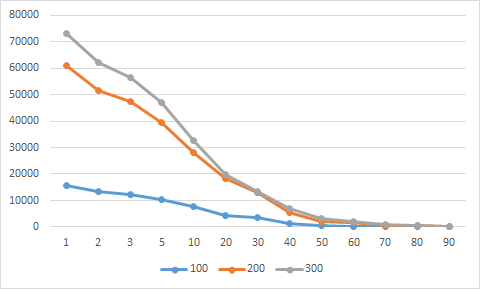
\includegraphics[scale=1]{imagenes/Experimental/DiferenciasGACEP.png}
        \caption{Gráfica asociada a la tabla \ref{DiferenciasGACEP}}
        \label{fig:DiferenciasGACEP}
\end{figure}

En la tabla \ref{DiferenciasGACEP} se puede ver que GACEP tiene un comportamiento similar con respecto a la progresión de las mejores soluciones a lo largo de la ejecución que el algoritmo base AGEU. 
Se observa que no se produce ninguna convergencia prematura, aunque es cierto que en la segunda mitad de las evaluaciones se producen muchos menos cambios que en el resto. 



\section{Uso de GRASP}

La modificación anterior tenía como objetivo aumentar la explotación de los buenos resultados. 
Para volver a conseguir un buen balance de explotación y exploración en el algoritmo lo siguiente que debemos pensar es qué clase de modificación se podría introducir de forma que aumentase la diversidad de la población y/o de las soluciones a considerar. 

La siguiente modificación que se plantea es la sustitución del uso del algoritmo Greedy por una variante suya: GRASP. 
Esta modificación solo tiene sentido usarla en el operador de reparación en la fase de aprendizaje del histórico. 
Esto es porque el único sitio donde se utiliza Greedy es en el operador de reparación, que intenta introducir siempre el mejor elemento a la solución y eliminar el peor. 
Durante la fase de acción del histórico ya realiza de por si un procedimiento similar al del GRASP, ya que le da prioridad a introducir alguno (sin comprobar si es verdaderamente el mejor) de los mejores elementos aprendidos y eliminar alguno (sin comprobar si verdaderamente es el peor) de los peores elementos aprendidos. 

El objetivo de esta modificación es introducir un operador que permita diversificar la población, eliminando el determinismo de siempre elegir las mismos elementos. 
De esta forma, somos capaces de darle más importancia a la parte de exploración del algoritmo, pero siempre manteniendo que las soluciones sigan intentando ser lo mejor posible. 

Los resultados de la ejecución del algoritmo GACEP con esta modificación pueden verse en la tabla \ref{GACEP_GRASP}. 


\begin{table}[]
\begin{tabular}{|cclccllll}
\hline
\rowcolor[HTML]{FFFFC7} 
\multicolumn{9}{|c|}{\cellcolor[HTML]{FFFFC7}GACEP+GRASP}                                                                                                                                                                                                                                                                                                                                                                                                                                                                                                                                                                              \\ \hline
\rowcolor[HTML]{F7EAC7} 
\multicolumn{1}{|c|}{\cellcolor[HTML]{F7EAC7}n}                               & \multicolumn{1}{c|}{\cellcolor[HTML]{F7EAC7}densidad}              & \multicolumn{1}{c|}{\cellcolor[HTML]{F7EAC7}Resultado} & \multicolumn{1}{c|}{\cellcolor[HTML]{F7EAC7}n}                               & \multicolumn{1}{c|}{\cellcolor[HTML]{F7EAC7}densidad}               & \multicolumn{1}{c|}{\cellcolor[HTML]{F7EAC7}Resultado} & \multicolumn{1}{c|}{\cellcolor[HTML]{F7EAC7}n}                               & \multicolumn{1}{c|}{\cellcolor[HTML]{F7EAC7}densidad}              & \multicolumn{1}{c|}{\cellcolor[HTML]{F7EAC7}Resultado} \\ \hline
\rowcolor[HTML]{DAE8FC} 
\multicolumn{1}{|c|}{\cellcolor[HTML]{FFFFC7}}                                & \multicolumn{1}{c|}{\cellcolor[HTML]{DAE8FC}}                      & \multicolumn{1}{l|}{\cellcolor[HTML]{DAE8FC}203870}    & \multicolumn{1}{c|}{\cellcolor[HTML]{FFFFC7}}                                & \multicolumn{1}{c|}{\cellcolor[HTML]{DAE8FC}}                       & \multicolumn{1}{l|}{\cellcolor[HTML]{DAE8FC}379570}    & \multicolumn{1}{c|}{\cellcolor[HTML]{FFFFC7}}                                & \multicolumn{1}{c|}{\cellcolor[HTML]{DAE8FC}}                      & \multicolumn{1}{l|}{\cellcolor[HTML]{DAE8FC}379471}    \\ \cline{3-3} \cline{6-6} \cline{9-9} 
\multicolumn{1}{|c|}{\cellcolor[HTML]{FFFFC7}}                                & \multicolumn{1}{c|}{\cellcolor[HTML]{DAE8FC}}                      & \multicolumn{1}{l|}{\cellcolor[HTML]{DDFDFF}88229.5}   & \multicolumn{1}{c|}{\cellcolor[HTML]{FFFFC7}}                                & \multicolumn{1}{c|}{\cellcolor[HTML]{DAE8FC}}                       & \multicolumn{1}{l|}{\cellcolor[HTML]{DDFDFF}958934}    & \multicolumn{1}{c|}{\cellcolor[HTML]{FFFFC7}}                                & \multicolumn{1}{c|}{\cellcolor[HTML]{DAE8FC}}                      & \multicolumn{1}{l|}{\cellcolor[HTML]{DDFDFF}30802.7}   \\ \cline{3-3} \cline{6-6} \cline{9-9} 
\rowcolor[HTML]{DAE8FC} 
\multicolumn{1}{|c|}{\cellcolor[HTML]{FFFFC7}}                                & \multicolumn{1}{c|}{\cellcolor[HTML]{DAE8FC}}                      & \multicolumn{1}{l|}{\cellcolor[HTML]{DAE8FC}202940}    & \multicolumn{1}{c|}{\cellcolor[HTML]{FFFFC7}}                                & \multicolumn{1}{c|}{\cellcolor[HTML]{DAE8FC}}                       & \multicolumn{1}{l|}{\cellcolor[HTML]{DAE8FC}315558}    & \multicolumn{1}{c|}{\cellcolor[HTML]{FFFFC7}}                                & \multicolumn{1}{c|}{\cellcolor[HTML]{DAE8FC}}                      & \multicolumn{1}{l|}{\cellcolor[HTML]{DAE8FC}269072}    \\ \cline{3-3} \cline{6-6} \cline{9-9} 
\multicolumn{1}{|c|}{\cellcolor[HTML]{FFFFC7}}                                & \multicolumn{1}{c|}{\cellcolor[HTML]{DAE8FC}}                      & \multicolumn{1}{l|}{\cellcolor[HTML]{DDFDFF}235610}    & \multicolumn{1}{c|}{\cellcolor[HTML]{FFFFC7}}                                & \multicolumn{1}{c|}{\cellcolor[HTML]{DAE8FC}}                       & \multicolumn{1}{l|}{\cellcolor[HTML]{DDFDFF}32375.5}   & \multicolumn{1}{c|}{\cellcolor[HTML]{FFFFC7}}                                & \multicolumn{1}{c|}{\cellcolor[HTML]{DAE8FC}}                      & \multicolumn{1}{l|}{\cellcolor[HTML]{DDFDFF}453902}    \\ \cline{3-3} \cline{6-6} \cline{9-9} 
\rowcolor[HTML]{DAE8FC} 
\multicolumn{1}{|c|}{\cellcolor[HTML]{FFFFC7}}                                & \multicolumn{1}{c|}{\cellcolor[HTML]{DAE8FC}}                      & \multicolumn{1}{l|}{\cellcolor[HTML]{DAE8FC}238439}    & \multicolumn{1}{c|}{\cellcolor[HTML]{FFFFC7}}                                & \multicolumn{1}{c|}{\cellcolor[HTML]{DAE8FC}}                       & \multicolumn{1}{l|}{\cellcolor[HTML]{DAE8FC}106229}    & \multicolumn{1}{c|}{\cellcolor[HTML]{FFFFC7}}                                & \multicolumn{1}{c|}{\cellcolor[HTML]{DAE8FC}}                      & \multicolumn{1}{l|}{\cellcolor[HTML]{DAE8FC}15967.4}   \\ \cline{3-3} \cline{6-6} \cline{9-9} 
\multicolumn{1}{|c|}{\cellcolor[HTML]{FFFFC7}}                                & \multicolumn{1}{c|}{\cellcolor[HTML]{DAE8FC}}                      & \multicolumn{1}{l|}{\cellcolor[HTML]{DDFDFF}81325.7}   & \multicolumn{1}{c|}{\cellcolor[HTML]{FFFFC7}}                                & \multicolumn{1}{c|}{\cellcolor[HTML]{DAE8FC}}                       & \multicolumn{1}{l|}{\cellcolor[HTML]{DDFDFF}813622}    & \multicolumn{1}{c|}{\cellcolor[HTML]{FFFFC7}}                                & \multicolumn{1}{c|}{\cellcolor[HTML]{DAE8FC}}                      & \multicolumn{1}{l|}{\cellcolor[HTML]{DDFDFF}253405}    \\ \cline{3-3} \cline{6-6} \cline{9-9} 
\rowcolor[HTML]{DAE8FC} 
\multicolumn{1}{|c|}{\cellcolor[HTML]{FFFFC7}}                                & \multicolumn{1}{c|}{\cellcolor[HTML]{DAE8FC}}                      & \multicolumn{1}{l|}{\cellcolor[HTML]{DAE8FC}10867.2}   & \multicolumn{1}{c|}{\cellcolor[HTML]{FFFFC7}}                                & \multicolumn{1}{c|}{\cellcolor[HTML]{DAE8FC}}                       & \multicolumn{1}{l|}{\cellcolor[HTML]{DAE8FC}44144.1}   & \multicolumn{1}{c|}{\cellcolor[HTML]{FFFFC7}}                                & \multicolumn{1}{c|}{\cellcolor[HTML]{DAE8FC}}                      & \multicolumn{1}{l|}{\cellcolor[HTML]{DAE8FC}494802}    \\ \cline{3-3} \cline{6-6} \cline{9-9} 
\multicolumn{1}{|c|}{\cellcolor[HTML]{FFFFC7}}                                & \multicolumn{1}{c|}{\cellcolor[HTML]{DAE8FC}}                      & \multicolumn{1}{l|}{\cellcolor[HTML]{DDFDFF}67669.3}   & \multicolumn{1}{c|}{\cellcolor[HTML]{FFFFC7}}                                & \multicolumn{1}{c|}{\cellcolor[HTML]{DAE8FC}}                       & \multicolumn{1}{l|}{\cellcolor[HTML]{DDFDFF}726019}    & \multicolumn{1}{c|}{\cellcolor[HTML]{FFFFC7}}                                & \multicolumn{1}{c|}{\cellcolor[HTML]{DAE8FC}}                      & \multicolumn{1}{l|}{\cellcolor[HTML]{DDFDFF}9783.9}    \\ \cline{3-3} \cline{6-6} \cline{9-9} 
\rowcolor[HTML]{DAE8FC} 
\multicolumn{1}{|c|}{\cellcolor[HTML]{FFFFC7}}                                & \multicolumn{1}{c|}{\cellcolor[HTML]{DAE8FC}}                      & \multicolumn{1}{l|}{\cellcolor[HTML]{DAE8FC}239982}    & \multicolumn{1}{c|}{\cellcolor[HTML]{FFFFC7}}                                & \multicolumn{1}{c|}{\multirow{-9}{*}{\cellcolor[HTML]{DAE8FC}25}}   & \multicolumn{1}{l|}{\cellcolor[HTML]{DAE8FC}813949}    & \multicolumn{1}{c|}{\cellcolor[HTML]{FFFFC7}}                                & \multicolumn{1}{c|}{\multirow{-9}{*}{\cellcolor[HTML]{DAE8FC}25}}  & \multicolumn{1}{l|}{\cellcolor[HTML]{DAE8FC}237551}    \\ \cline{3-3} \cline{5-6} \cline{8-9} 
\multicolumn{1}{|c|}{\cellcolor[HTML]{FFFFC7}}                                & \multicolumn{1}{c|}{\multirow{-10}{*}{\cellcolor[HTML]{DAE8FC}25}} & \multicolumn{1}{l|}{\cellcolor[HTML]{DDFDFF}26642.1}   & \multicolumn{1}{c|}{\cellcolor[HTML]{FFFFC7}}                                & \multicolumn{1}{c|}{\cellcolor[HTML]{DDFDFF}}                       & \multicolumn{1}{l|}{\cellcolor[HTML]{DAE8FC}653176}    & \multicolumn{1}{c|}{\cellcolor[HTML]{FFFFC7}}                                & \multicolumn{1}{c|}{\cellcolor[HTML]{DDFDFF}}                      & \multicolumn{1}{l|}{\cellcolor[HTML]{DAE8FC}1017990}   \\ \cline{2-3} \cline{6-6} \cline{9-9} 
\rowcolor[HTML]{DDFDFF} 
\multicolumn{1}{|c|}{\cellcolor[HTML]{FFFFC7}}                                & \multicolumn{1}{c|}{\cellcolor[HTML]{DDFDFF}}                      & \multicolumn{1}{l|}{\cellcolor[HTML]{DAE8FC}20217.6}   & \multicolumn{1}{c|}{\cellcolor[HTML]{FFFFC7}}                                & \multicolumn{1}{c|}{\cellcolor[HTML]{DDFDFF}}                       & \multicolumn{1}{l|}{\cellcolor[HTML]{DDFDFF}50543}     & \multicolumn{1}{c|}{\cellcolor[HTML]{FFFFC7}}                                & \multicolumn{1}{c|}{\cellcolor[HTML]{DDFDFF}}                      & \multicolumn{1}{l|}{\cellcolor[HTML]{DDFDFF}483693}    \\ \cline{3-3} \cline{6-6} \cline{9-9} 
\multicolumn{1}{|c|}{\cellcolor[HTML]{FFFFC7}}                                & \multicolumn{1}{c|}{\cellcolor[HTML]{DDFDFF}}                      & \multicolumn{1}{l|}{\cellcolor[HTML]{DDFDFF}58173.8}   & \multicolumn{1}{c|}{\cellcolor[HTML]{FFFFC7}}                                & \multicolumn{1}{c|}{\cellcolor[HTML]{DDFDFF}}                       & \multicolumn{1}{l|}{\cellcolor[HTML]{DAE8FC}211429}    & \multicolumn{1}{c|}{\cellcolor[HTML]{FFFFC7}}                                & \multicolumn{1}{c|}{\cellcolor[HTML]{DDFDFF}}                      & \multicolumn{1}{l|}{\cellcolor[HTML]{DAE8FC}110079}    \\ \cline{3-3} \cline{6-6} \cline{9-9} 
\rowcolor[HTML]{DDFDFF} 
\multicolumn{1}{|c|}{\cellcolor[HTML]{FFFFC7}}                                & \multicolumn{1}{c|}{\cellcolor[HTML]{DDFDFF}}                      & \multicolumn{1}{l|}{\cellcolor[HTML]{DAE8FC}3967.14}   & \multicolumn{1}{c|}{\cellcolor[HTML]{FFFFC7}}                                & \multicolumn{1}{c|}{\cellcolor[HTML]{DDFDFF}}                       & \multicolumn{1}{l|}{\cellcolor[HTML]{DDFDFF}244518}    & \multicolumn{1}{c|}{\cellcolor[HTML]{FFFFC7}}                                & \multicolumn{1}{c|}{\cellcolor[HTML]{DDFDFF}}                      & \multicolumn{1}{l|}{\cellcolor[HTML]{DDFDFF}890216}    \\ \cline{3-3} \cline{6-6} \cline{9-9} 
\multicolumn{1}{|c|}{\cellcolor[HTML]{FFFFC7}}                                & \multicolumn{1}{c|}{\cellcolor[HTML]{DDFDFF}}                      & \multicolumn{1}{l|}{\cellcolor[HTML]{DDFDFF}53183.3}   & \multicolumn{1}{c|}{\cellcolor[HTML]{FFFFC7}}                                & \multicolumn{1}{c|}{\cellcolor[HTML]{DDFDFF}}                       & \multicolumn{1}{l|}{\cellcolor[HTML]{DAE8FC}227361}    & \multicolumn{1}{c|}{\cellcolor[HTML]{FFFFC7}}                                & \multicolumn{1}{c|}{\cellcolor[HTML]{DDFDFF}}                      & \multicolumn{1}{l|}{\cellcolor[HTML]{DAE8FC}310174}    \\ \cline{3-3} \cline{6-6} \cline{9-9} 
\rowcolor[HTML]{DDFDFF} 
\multicolumn{1}{|c|}{\cellcolor[HTML]{FFFFC7}}                                & \multicolumn{1}{c|}{\cellcolor[HTML]{DDFDFF}}                      & \multicolumn{1}{l|}{\cellcolor[HTML]{DAE8FC}62310.9}   & \multicolumn{1}{c|}{\cellcolor[HTML]{FFFFC7}}                                & \multicolumn{1}{c|}{\cellcolor[HTML]{DDFDFF}}                       & \multicolumn{1}{l|}{\cellcolor[HTML]{DDFDFF}193634}    & \multicolumn{1}{c|}{\cellcolor[HTML]{FFFFC7}}                                & \multicolumn{1}{c|}{\cellcolor[HTML]{DDFDFF}}                      & \multicolumn{1}{l|}{\cellcolor[HTML]{DDFDFF}722245}    \\ \cline{3-3} \cline{6-6} \cline{9-9} 
\multicolumn{1}{|c|}{\cellcolor[HTML]{FFFFC7}}                                & \multicolumn{1}{c|}{\cellcolor[HTML]{DDFDFF}}                      & \multicolumn{1}{l|}{\cellcolor[HTML]{DDFDFF}38963}     & \multicolumn{1}{c|}{\cellcolor[HTML]{FFFFC7}}                                & \multicolumn{1}{c|}{\cellcolor[HTML]{DDFDFF}}                       & \multicolumn{1}{l|}{\cellcolor[HTML]{DAE8FC}81477.9}   & \multicolumn{1}{c|}{\cellcolor[HTML]{FFFFC7}}                                & \multicolumn{1}{c|}{\cellcolor[HTML]{DDFDFF}}                      & \multicolumn{1}{l|}{\cellcolor[HTML]{DAE8FC}738970}    \\ \cline{3-3} \cline{6-6} \cline{9-9} 
\rowcolor[HTML]{DDFDFF} 
\multicolumn{1}{|c|}{\cellcolor[HTML]{FFFFC7}}                                & \multicolumn{1}{c|}{\cellcolor[HTML]{DDFDFF}}                      & \multicolumn{1}{l|}{\cellcolor[HTML]{DAE8FC}15641.2}   & \multicolumn{1}{c|}{\cellcolor[HTML]{FFFFC7}}                                & \multicolumn{1}{c|}{\cellcolor[HTML]{DDFDFF}}                       & \multicolumn{1}{l|}{\cellcolor[HTML]{DDFDFF}61504}     & \multicolumn{1}{c|}{\cellcolor[HTML]{FFFFC7}}                                & \multicolumn{1}{c|}{\cellcolor[HTML]{DDFDFF}}                      & \multicolumn{1}{l|}{\cellcolor[HTML]{DDFDFF}46951.9}   \\ \cline{3-3} \cline{6-6} \cline{9-9} 
\multicolumn{1}{|c|}{\cellcolor[HTML]{FFFFC7}}                                & \multicolumn{1}{c|}{\cellcolor[HTML]{DDFDFF}}                      & \multicolumn{1}{l|}{\cellcolor[HTML]{DDFDFF}22181.6}   & \multicolumn{1}{c|}{\cellcolor[HTML]{FFFFC7}}                                & \multicolumn{1}{c|}{\cellcolor[HTML]{DDFDFF}}                       & \multicolumn{1}{l|}{\cellcolor[HTML]{DAE8FC}150655}    & \multicolumn{1}{c|}{\cellcolor[HTML]{FFFFC7}}                                & \multicolumn{1}{c|}{\cellcolor[HTML]{DDFDFF}}                      & \multicolumn{1}{l|}{\cellcolor[HTML]{DAE8FC}770539}    \\ \cline{3-3} \cline{6-6} \cline{9-9} 
\rowcolor[HTML]{DDFDFF} 
\multicolumn{1}{|c|}{\cellcolor[HTML]{FFFFC7}}                                & \multicolumn{1}{c|}{\cellcolor[HTML]{DDFDFF}}                      & \multicolumn{1}{l|}{\cellcolor[HTML]{DAE8FC}37575.9}   & \multicolumn{1}{c|}{\cellcolor[HTML]{FFFFC7}}                                & \multicolumn{1}{c|}{\multirow{-10}{*}{\cellcolor[HTML]{DDFDFF}50}}  & \multicolumn{1}{l|}{\cellcolor[HTML]{DDFDFF}51459}     & \multicolumn{1}{c|}{\multirow{-19}{*}{\cellcolor[HTML]{FFFFC7}\textbf{300}}} & \multicolumn{1}{c|}{\multirow{-10}{*}{\cellcolor[HTML]{DDFDFF}50}} & \multicolumn{1}{l|}{\cellcolor[HTML]{DDFDFF}766150}    \\ \cline{3-3} \cline{5-9} 
\multicolumn{1}{|c|}{\cellcolor[HTML]{FFFFC7}}                                & \multicolumn{1}{c|}{\multirow{-10}{*}{\cellcolor[HTML]{DDFDFF}50}} & \multicolumn{1}{l|}{\cellcolor[HTML]{DDFDFF}94259.5}   & \multicolumn{1}{c|}{\cellcolor[HTML]{FFFFC7}}                                & \multicolumn{1}{c|}{\cellcolor[HTML]{DAE8FC}}                       & \multicolumn{1}{l|}{\cellcolor[HTML]{DAE8FC}287285}    &                                                                              &                                                                    &                                                        \\ \cline{2-3} \cline{6-6}
\multicolumn{1}{|c|}{\cellcolor[HTML]{FFFFC7}}                                & \multicolumn{1}{c|}{\cellcolor[HTML]{DAE8FC}}                      & \multicolumn{1}{l|}{\cellcolor[HTML]{DAE8FC}89232.8}   & \multicolumn{1}{c|}{\cellcolor[HTML]{FFFFC7}}                                & \multicolumn{1}{c|}{\cellcolor[HTML]{DAE8FC}}                       & \multicolumn{1}{l|}{\cellcolor[HTML]{DDFDFF}383329}    &                                                                              &                                                                    &                                                        \\ \cline{3-3} \cline{6-6}
\multicolumn{1}{|c|}{\cellcolor[HTML]{FFFFC7}}                                & \multicolumn{1}{c|}{\cellcolor[HTML]{DAE8FC}}                      & \multicolumn{1}{l|}{\cellcolor[HTML]{DDFDFF}110642}    & \multicolumn{1}{c|}{\cellcolor[HTML]{FFFFC7}}                                & \multicolumn{1}{c|}{\cellcolor[HTML]{DAE8FC}}                       & \multicolumn{1}{l|}{\cellcolor[HTML]{DAE8FC}214848}    &                                                                              &                                                                    &                                                        \\ \cline{3-3} \cline{6-6}
\multicolumn{1}{|c|}{\cellcolor[HTML]{FFFFC7}}                                & \multicolumn{1}{c|}{\cellcolor[HTML]{DAE8FC}}                      & \multicolumn{1}{l|}{\cellcolor[HTML]{DAE8FC}37247.4}   & \multicolumn{1}{c|}{\cellcolor[HTML]{FFFFC7}}                                & \multicolumn{1}{c|}{\cellcolor[HTML]{DAE8FC}}                       & \multicolumn{1}{l|}{\cellcolor[HTML]{DDFDFF}225192}    &                                                                              &                                                                    &                                                        \\ \cline{3-3} \cline{6-6}
\multicolumn{1}{|c|}{\cellcolor[HTML]{FFFFC7}}                                & \multicolumn{1}{c|}{\cellcolor[HTML]{DAE8FC}}                      & \multicolumn{1}{l|}{\cellcolor[HTML]{DDFDFF}110026}    & \multicolumn{1}{c|}{\cellcolor[HTML]{FFFFC7}}                                & \multicolumn{1}{c|}{\cellcolor[HTML]{DAE8FC}}                       & \multicolumn{1}{l|}{\cellcolor[HTML]{DAE8FC}225684}    &                                                                              &                                                                    &                                                        \\ \cline{3-3} \cline{6-6}
\multicolumn{1}{|c|}{\cellcolor[HTML]{FFFFC7}}                                & \multicolumn{1}{c|}{\cellcolor[HTML]{DAE8FC}}                      & \multicolumn{1}{l|}{\cellcolor[HTML]{DAE8FC}60821.5}   & \multicolumn{1}{c|}{\cellcolor[HTML]{FFFFC7}}                                & \multicolumn{1}{c|}{\cellcolor[HTML]{DAE8FC}}                       & \multicolumn{1}{l|}{\cellcolor[HTML]{DDFDFF}489291}    &                                                                              &                                                                    &                                                        \\ \cline{3-3} \cline{6-6}
\multicolumn{1}{|c|}{\cellcolor[HTML]{FFFFC7}}                                & \multicolumn{1}{c|}{\cellcolor[HTML]{DAE8FC}}                      & \multicolumn{1}{l|}{\cellcolor[HTML]{DDFDFF}18066.4}   & \multicolumn{1}{c|}{\cellcolor[HTML]{FFFFC7}}                                & \multicolumn{1}{c|}{\cellcolor[HTML]{DAE8FC}}                       & \multicolumn{1}{l|}{\cellcolor[HTML]{DAE8FC}440828}    &                                                                              &                                                                    &                                                        \\ \cline{3-3} \cline{6-6}
\multicolumn{1}{|c|}{\cellcolor[HTML]{FFFFC7}}                                & \multicolumn{1}{c|}{\cellcolor[HTML]{DAE8FC}}                      & \multicolumn{1}{l|}{\cellcolor[HTML]{DAE8FC}55937.8}   & \multicolumn{1}{c|}{\cellcolor[HTML]{FFFFC7}}                                & \multicolumn{1}{c|}{\cellcolor[HTML]{DAE8FC}}                       & \multicolumn{1}{l|}{\cellcolor[HTML]{DDFDFF}220101}    &                                                                              &                                                                    &                                                        \\ \cline{3-3} \cline{6-6}
\multicolumn{1}{|c|}{\cellcolor[HTML]{FFFFC7}}                                & \multicolumn{1}{c|}{\cellcolor[HTML]{DAE8FC}}                      & \multicolumn{1}{l|}{\cellcolor[HTML]{DDFDFF}58848.7}   & \multicolumn{1}{c|}{\cellcolor[HTML]{FFFFC7}}                                & \multicolumn{1}{c|}{\cellcolor[HTML]{DAE8FC}}                       & \multicolumn{1}{l|}{\cellcolor[HTML]{DAE8FC}324902}    &                                                                              &                                                                    &                                                        \\ \cline{3-3} \cline{6-6}
\multicolumn{1}{|c|}{\cellcolor[HTML]{FFFFC7}}                                & \multicolumn{1}{c|}{\cellcolor[HTML]{DAE8FC}}                      & \multicolumn{1}{l|}{\cellcolor[HTML]{DAE8FC}73569.8}   & \multicolumn{1}{c|}{\cellcolor[HTML]{FFFFC7}}                                & \multicolumn{1}{c|}{\multirow{-10}{*}{\cellcolor[HTML]{DAE8FC}75}}  & \multicolumn{1}{l|}{\cellcolor[HTML]{DDFDFF}110572}    &                                                                              &                                                                    &                                                        \\ \cline{3-3} \cline{5-6}
\multicolumn{1}{|c|}{\cellcolor[HTML]{FFFFC7}}                                & \multicolumn{1}{c|}{\multirow{-10}{*}{\cellcolor[HTML]{DAE8FC}75}} & \multicolumn{1}{l|}{\cellcolor[HTML]{DDFDFF}151250}    & \multicolumn{1}{c|}{\cellcolor[HTML]{FFFFC7}}                                & \multicolumn{1}{c|}{\cellcolor[HTML]{DDFDFF}}                       & \multicolumn{1}{l|}{\cellcolor[HTML]{DAE8FC}150784}    &                                                                              &                                                                    &                                                        \\ \cline{2-3} \cline{6-6}
\multicolumn{1}{|c|}{\cellcolor[HTML]{FFFFC7}}                                & \multicolumn{1}{c|}{\cellcolor[HTML]{DDFDFF}}                      & \multicolumn{1}{l|}{\cellcolor[HTML]{DAE8FC}191323}    & \multicolumn{1}{c|}{\cellcolor[HTML]{FFFFC7}}                                & \multicolumn{1}{c|}{\cellcolor[HTML]{DDFDFF}}                       & \multicolumn{1}{l|}{\cellcolor[HTML]{DDFDFF}452607}    &                                                                              &                                                                    &                                                        \\ \cline{3-3} \cline{6-6}
\multicolumn{1}{|c|}{\cellcolor[HTML]{FFFFC7}}                                & \multicolumn{1}{c|}{\cellcolor[HTML]{DDFDFF}}                      & \multicolumn{1}{l|}{\cellcolor[HTML]{DDFDFF}104160}    & \multicolumn{1}{c|}{\cellcolor[HTML]{FFFFC7}}                                & \multicolumn{1}{c|}{\cellcolor[HTML]{DDFDFF}}                       & \multicolumn{1}{l|}{\cellcolor[HTML]{DAE8FC}281795}    &                                                                              &                                                                    &                                                        \\ \cline{3-3} \cline{6-6}
\multicolumn{1}{|c|}{\cellcolor[HTML]{FFFFC7}}                                & \multicolumn{1}{c|}{\cellcolor[HTML]{DDFDFF}}                      & \multicolumn{1}{l|}{\cellcolor[HTML]{DAE8FC}66522.7}   & \multicolumn{1}{c|}{\cellcolor[HTML]{FFFFC7}}                                & \multicolumn{1}{c|}{\cellcolor[HTML]{DDFDFF}}                       & \multicolumn{1}{l|}{\cellcolor[HTML]{DDFDFF}66610.6}   &                                                                              &                                                                    &                                                        \\ \cline{3-3} \cline{6-6}
\multicolumn{1}{|c|}{\cellcolor[HTML]{FFFFC7}}                                & \multicolumn{1}{c|}{\cellcolor[HTML]{DDFDFF}}                      & \multicolumn{1}{l|}{\cellcolor[HTML]{DDFDFF}80481.7}   & \multicolumn{1}{c|}{\cellcolor[HTML]{FFFFC7}}                                & \multicolumn{1}{c|}{\cellcolor[HTML]{DDFDFF}}                       & \multicolumn{1}{l|}{\cellcolor[HTML]{DAE8FC}133906}    &                                                                              &                                                                    &                                                        \\ \cline{3-3} \cline{6-6}
\multicolumn{1}{|c|}{\cellcolor[HTML]{FFFFC7}}                                & \multicolumn{1}{c|}{\cellcolor[HTML]{DDFDFF}}                      & \multicolumn{1}{l|}{\cellcolor[HTML]{DAE8FC}31122.7}   & \multicolumn{1}{c|}{\cellcolor[HTML]{FFFFC7}}                                & \multicolumn{1}{c|}{\cellcolor[HTML]{DDFDFF}}                       & \multicolumn{1}{l|}{\cellcolor[HTML]{DDFDFF}146870}    &                                                                              &                                                                    &                                                        \\ \cline{3-3} \cline{6-6}
\multicolumn{1}{|c|}{\cellcolor[HTML]{FFFFC7}}                                & \multicolumn{1}{c|}{\cellcolor[HTML]{DDFDFF}}                      & \multicolumn{1}{l|}{\cellcolor[HTML]{DDFDFF}153157}    & \multicolumn{1}{c|}{\cellcolor[HTML]{FFFFC7}}                                & \multicolumn{1}{c|}{\cellcolor[HTML]{DDFDFF}}                       & \multicolumn{1}{l|}{\cellcolor[HTML]{DAE8FC}234757}    &                                                                              &                                                                    &                                                        \\ \cline{3-3} \cline{6-6}
\multicolumn{1}{|c|}{\cellcolor[HTML]{FFFFC7}}                                & \multicolumn{1}{c|}{\cellcolor[HTML]{DDFDFF}}                      & \multicolumn{1}{l|}{\cellcolor[HTML]{DAE8FC}120369}    & \multicolumn{1}{c|}{\cellcolor[HTML]{FFFFC7}}                                & \multicolumn{1}{c|}{\cellcolor[HTML]{DDFDFF}}                       & \multicolumn{1}{l|}{\cellcolor[HTML]{DDFDFF}275504}    &                                                                              &                                                                    &                                                        \\ \cline{3-3} \cline{6-6}
\multicolumn{1}{|c|}{\cellcolor[HTML]{FFFFC7}}                                & \multicolumn{1}{c|}{\cellcolor[HTML]{DDFDFF}}                      & \multicolumn{1}{l|}{\cellcolor[HTML]{DDFDFF}21816.6}   & \multicolumn{1}{c|}{\cellcolor[HTML]{FFFFC7}}                                & \multicolumn{1}{c|}{\cellcolor[HTML]{DDFDFF}}                       & \multicolumn{1}{l|}{\cellcolor[HTML]{DAE8FC}620630}    &                                                                              &                                                                    &                                                        \\ \cline{3-3} \cline{6-6}
\multicolumn{1}{|c|}{\multirow{-39}{*}{\cellcolor[HTML]{FFFFC7}\textbf{100}}} & \multicolumn{1}{c|}{\multirow{-9}{*}{\cellcolor[HTML]{DDFDFF}100}} & \multicolumn{1}{l|}{\cellcolor[HTML]{DAE8FC}112427}    & \multicolumn{1}{c|}{\multirow{-39}{*}{\cellcolor[HTML]{FFFFC7}\textbf{200}}} & \multicolumn{1}{c|}{\multirow{-10}{*}{\cellcolor[HTML]{DDFDFF}100}} & \multicolumn{1}{l|}{\cellcolor[HTML]{DDFDFF}534844}    &                                                                              &                                                                    &                                                        \\ \cline{1-6}
\end{tabular}
\caption{\label{GACEP_GRASP}Resultados de la ejecución de GACEP+GRASP}
\end{table}

Con esto, debemos comprobar si realmente se ha producido una mejora con respecto a la modificación anterior. 
Para ello compararemos sus resultados y estableceremos un \textit{ranking}, siendo la gráfica correspondiente a esta comparación la gráfica \ref{fig:GRASPvswoGRASP}. 
Donde la etiqueta ``wGRASP'' indica la versión de GACEP a la que se le ha introducido GRASP y la etiqueta ``woGRASP'' indica la versión de GACEP anterior (solo histórico). 

\begin{figure}[h]
		\centering
		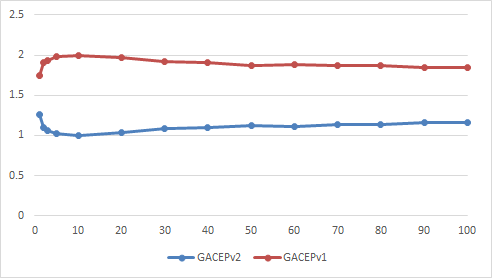
\includegraphics[scale=1]{imagenes/Experimental/GRASPvswoGRASP.png}
        \caption{Comparación de los resultados del GACEP y la aplicación de GRASP}
        \label{fig:GRASPvswoGRASP}
\end{figure}

En esta gráfica \ref{fig:GRASPvswoGRASP} se puede ver cómo la nueva versión, introduciendo GRASP, es consistentemente mejor que la versión anterior. 
Es más, se puede afirmar que es mejor en casi todos los datos utilizados. 
Por lo tanto, se procederá a continuar con el desarrollo de nuestro algoritmo sobre esta nueva versión.

A continuación, se mostrará una tabla \ref{DiferenciasGACEP_GRASP} que almacena la media de las diferencias de los resultados de cada \textit{milestone} con respecto a la final, con el fin de comprobar si podemos sacar información sobre la convergencia de las soluciones en el tiempo. 

\begin{table}[h]
\begin{tabular}{|cclcclccl|}
\hline
\rowcolor[HTML]{FFFFC7} 
\multicolumn{9}{|c|}{\cellcolor[HTML]{FFFFC7}GACEP}                                                                                                                                                                                                                                                                                                                                                                                                                                                                                                       \\ \hline
\rowcolor[HTML]{F7EAC7} 
\multicolumn{1}{|c|}{\cellcolor[HTML]{F7EAC7}n}                               & \multicolumn{1}{c|}{\cellcolor[HTML]{F7EAC7}milestone} & \multicolumn{1}{c|}{\cellcolor[HTML]{F7EAC7}Diferencia} & \multicolumn{1}{c|}{\cellcolor[HTML]{F7EAC7}n}                               & \multicolumn{1}{c|}{\cellcolor[HTML]{F7EAC7}milestone} & \multicolumn{1}{l|}{\cellcolor[HTML]{F7EAC7}Diferencia}  & \multicolumn{1}{c|}{\cellcolor[HTML]{F7EAC7}n}                               & \multicolumn{1}{c|}{\cellcolor[HTML]{F7EAC7}milestone} & Diferencia  \\ \hline
\rowcolor[HTML]{DAE8FC} 
\multicolumn{1}{|c|}{\cellcolor[HTML]{FFFFC7}}                                & \multicolumn{1}{c|}{\cellcolor[HTML]{DAE8FC}1}         & \multicolumn{1}{l|}{\cellcolor[HTML]{DAE8FC}15809.47}   & \multicolumn{1}{c|}{\cellcolor[HTML]{FFFFC7}}                                & \multicolumn{1}{c|}{\cellcolor[HTML]{DAE8FC}1}         & \multicolumn{1}{l|}{\cellcolor[HTML]{DAE8FC}64364.05641} & \multicolumn{1}{c|}{\cellcolor[HTML]{FFFFC7}}                                & \multicolumn{1}{c|}{\cellcolor[HTML]{DAE8FC}1}         & 80461.67684 \\ \cline{2-3} \cline{5-6} \cline{8-9} 
\rowcolor[HTML]{DDFDFF} 
\multicolumn{1}{|c|}{\cellcolor[HTML]{FFFFC7}}                                & \multicolumn{1}{c|}{\cellcolor[HTML]{DDFDFF}2}         & \multicolumn{1}{l|}{\cellcolor[HTML]{DDFDFF}13375.28}   & \multicolumn{1}{c|}{\cellcolor[HTML]{FFFFC7}}                                & \multicolumn{1}{c|}{\cellcolor[HTML]{DDFDFF}2}         & \multicolumn{1}{l|}{\cellcolor[HTML]{DDFDFF}54276.43333} & \multicolumn{1}{c|}{\cellcolor[HTML]{FFFFC7}}                                & \multicolumn{1}{c|}{\cellcolor[HTML]{DDFDFF}2}         & 69283.33053 \\ \cline{2-3} \cline{5-6} \cline{8-9} 
\rowcolor[HTML]{DAE8FC} 
\multicolumn{1}{|c|}{\cellcolor[HTML]{FFFFC7}}                                & \multicolumn{1}{c|}{\cellcolor[HTML]{DAE8FC}3}         & \multicolumn{1}{l|}{\cellcolor[HTML]{DAE8FC}12160.14}   & \multicolumn{1}{c|}{\cellcolor[HTML]{FFFFC7}}                                & \multicolumn{1}{c|}{\cellcolor[HTML]{DAE8FC}3}         & \multicolumn{1}{l|}{\cellcolor[HTML]{DAE8FC}49560.91026} & \multicolumn{1}{c|}{\cellcolor[HTML]{FFFFC7}}                                & \multicolumn{1}{c|}{\cellcolor[HTML]{DAE8FC}3}         & 62840.55684 \\ \cline{2-3} \cline{5-6} \cline{8-9} 
\rowcolor[HTML]{DDFDFF} 
\multicolumn{1}{|c|}{\cellcolor[HTML]{FFFFC7}}                                & \multicolumn{1}{c|}{\cellcolor[HTML]{DDFDFF}5}         & \multicolumn{1}{l|}{\cellcolor[HTML]{DDFDFF}10129.33}   & \multicolumn{1}{c|}{\cellcolor[HTML]{FFFFC7}}                                & \multicolumn{1}{c|}{\cellcolor[HTML]{DDFDFF}5}         & \multicolumn{1}{l|}{\cellcolor[HTML]{DDFDFF}40912.41282} & \multicolumn{1}{c|}{\cellcolor[HTML]{FFFFC7}}                                & \multicolumn{1}{c|}{\cellcolor[HTML]{DDFDFF}5}         & 52458.6     \\ \cline{2-3} \cline{5-6} \cline{8-9} 
\rowcolor[HTML]{DAE8FC} 
\multicolumn{1}{|c|}{\cellcolor[HTML]{FFFFC7}}                                & \multicolumn{1}{c|}{\cellcolor[HTML]{DAE8FC}10}        & \multicolumn{1}{l|}{\cellcolor[HTML]{DAE8FC}7377.82}    & \multicolumn{1}{c|}{\cellcolor[HTML]{FFFFC7}}                                & \multicolumn{1}{c|}{\cellcolor[HTML]{DAE8FC}10}        & \multicolumn{1}{l|}{\cellcolor[HTML]{DAE8FC}28323.05128} & \multicolumn{1}{c|}{\cellcolor[HTML]{FFFFC7}}                                & \multicolumn{1}{c|}{\cellcolor[HTML]{DAE8FC}10}        & 35701.50526 \\ \cline{2-3} \cline{5-6} \cline{8-9} 
\rowcolor[HTML]{DDFDFF} 
\multicolumn{1}{|c|}{\cellcolor[HTML]{FFFFC7}}                                & \multicolumn{1}{c|}{\cellcolor[HTML]{DDFDFF}20}        & \multicolumn{1}{l|}{\cellcolor[HTML]{DDFDFF}4346.69}    & \multicolumn{1}{c|}{\cellcolor[HTML]{FFFFC7}}                                & \multicolumn{1}{c|}{\cellcolor[HTML]{DDFDFF}20}        & \multicolumn{1}{l|}{\cellcolor[HTML]{DDFDFF}18539.38718} & \multicolumn{1}{c|}{\cellcolor[HTML]{FFFFC7}}                                & \multicolumn{1}{c|}{\cellcolor[HTML]{DDFDFF}20}        & 22524.66947 \\ \cline{2-3} \cline{5-6} \cline{8-9} 
\rowcolor[HTML]{DAE8FC} 
\multicolumn{1}{|c|}{\cellcolor[HTML]{FFFFC7}}                                & \multicolumn{1}{c|}{\cellcolor[HTML]{DAE8FC}30}        & \multicolumn{1}{l|}{\cellcolor[HTML]{DAE8FC}3569.00}    & \multicolumn{1}{c|}{\cellcolor[HTML]{FFFFC7}}                                & \multicolumn{1}{c|}{\cellcolor[HTML]{DAE8FC}30}        & \multicolumn{1}{l|}{\cellcolor[HTML]{DAE8FC}13126.02564} & \multicolumn{1}{c|}{\cellcolor[HTML]{FFFFC7}}                                & \multicolumn{1}{c|}{\cellcolor[HTML]{DAE8FC}30}        & 15350.76105 \\ \cline{2-3} \cline{5-6} \cline{8-9} 
\rowcolor[HTML]{DDFDFF} 
\multicolumn{1}{|c|}{\cellcolor[HTML]{FFFFC7}}                                & \multicolumn{1}{c|}{\cellcolor[HTML]{DDFDFF}40}        & \multicolumn{1}{l|}{\cellcolor[HTML]{DDFDFF}652.75}     & \multicolumn{1}{c|}{\cellcolor[HTML]{FFFFC7}}                                & \multicolumn{1}{c|}{\cellcolor[HTML]{DDFDFF}40}        & \multicolumn{1}{l|}{\cellcolor[HTML]{DDFDFF}4891.348718} & \multicolumn{1}{c|}{\cellcolor[HTML]{FFFFC7}}                                & \multicolumn{1}{c|}{\cellcolor[HTML]{DDFDFF}40}        & 7703.853684 \\ \cline{2-3} \cline{5-6} \cline{8-9} 
\rowcolor[HTML]{DAE8FC} 
\multicolumn{1}{|c|}{\cellcolor[HTML]{FFFFC7}}                                & \multicolumn{1}{c|}{\cellcolor[HTML]{DAE8FC}50}        & \multicolumn{1}{l|}{\cellcolor[HTML]{DAE8FC}231.25}     & \multicolumn{1}{c|}{\cellcolor[HTML]{FFFFC7}}                                & \multicolumn{1}{c|}{\cellcolor[HTML]{DAE8FC}50}        & \multicolumn{1}{l|}{\cellcolor[HTML]{DAE8FC}2075.925641} & \multicolumn{1}{c|}{\cellcolor[HTML]{FFFFC7}}                                & \multicolumn{1}{c|}{\cellcolor[HTML]{DAE8FC}50}        & 4243.413684 \\ \cline{2-3} \cline{5-6} \cline{8-9} 
\rowcolor[HTML]{DDFDFF} 
\multicolumn{1}{|c|}{\cellcolor[HTML]{FFFFC7}}                                & \multicolumn{1}{c|}{\cellcolor[HTML]{DDFDFF}60}        & \multicolumn{1}{l|}{\cellcolor[HTML]{DDFDFF}68.21}      & \multicolumn{1}{c|}{\cellcolor[HTML]{FFFFC7}}                                & \multicolumn{1}{c|}{\cellcolor[HTML]{DDFDFF}60}        & \multicolumn{1}{l|}{\cellcolor[HTML]{DDFDFF}708.6923077} & \multicolumn{1}{c|}{\cellcolor[HTML]{FFFFC7}}                                & \multicolumn{1}{c|}{\cellcolor[HTML]{DDFDFF}60}        & 2096.854737 \\ \cline{2-3} \cline{5-6} \cline{8-9} 
\rowcolor[HTML]{DAE8FC} 
\multicolumn{1}{|c|}{\cellcolor[HTML]{FFFFC7}}                                & \multicolumn{1}{c|}{\cellcolor[HTML]{DAE8FC}70}        & \multicolumn{1}{l|}{\cellcolor[HTML]{DAE8FC}25.82}      & \multicolumn{1}{c|}{\cellcolor[HTML]{FFFFC7}}                                & \multicolumn{1}{c|}{\cellcolor[HTML]{DAE8FC}70}        & \multicolumn{1}{l|}{\cellcolor[HTML]{DAE8FC}135.7435897} & \multicolumn{1}{c|}{\cellcolor[HTML]{FFFFC7}}                                & \multicolumn{1}{c|}{\cellcolor[HTML]{DAE8FC}70}        & 669.4642105 \\ \cline{2-3} \cline{5-6} \cline{8-9} 
\rowcolor[HTML]{DDFDFF} 
\multicolumn{1}{|c|}{\cellcolor[HTML]{FFFFC7}}                                & \multicolumn{1}{c|}{\cellcolor[HTML]{DDFDFF}80}        & \multicolumn{1}{l|}{\cellcolor[HTML]{DDFDFF}5.61}       & \multicolumn{1}{c|}{\cellcolor[HTML]{FFFFC7}}                                & \multicolumn{1}{c|}{\cellcolor[HTML]{DDFDFF}80}        & \multicolumn{1}{l|}{\cellcolor[HTML]{DDFDFF}63.22564103} & \multicolumn{1}{c|}{\cellcolor[HTML]{FFFFC7}}                                & \multicolumn{1}{c|}{\cellcolor[HTML]{DDFDFF}80}        & 372.7431579 \\ \cline{2-3} \cline{5-6} \cline{8-9} 
\rowcolor[HTML]{DAE8FC} 
\multicolumn{1}{|c|}{\multirow{-13}{*}{\cellcolor[HTML]{FFFFC7}\textbf{100}}} & \multicolumn{1}{c|}{\cellcolor[HTML]{DAE8FC}90}        & \multicolumn{1}{l|}{\cellcolor[HTML]{DAE8FC}-0.30}      & \multicolumn{1}{c|}{\multirow{-13}{*}{\cellcolor[HTML]{FFFFC7}\textbf{200}}} & \multicolumn{1}{c|}{\cellcolor[HTML]{DAE8FC}90}        & \multicolumn{1}{l|}{\cellcolor[HTML]{DAE8FC}0}           & \multicolumn{1}{c|}{\multirow{-13}{*}{\cellcolor[HTML]{FFFFC7}\textbf{300}}} & \multicolumn{1}{c|}{\cellcolor[HTML]{DAE8FC}90}        & 1.789473684 \\ \hline
\end{tabular}
\caption{\label{DiferenciasGACEP_GRASP}Diferencias de los resultados de las distintas milestones con respecto a la final para el algoritmo GACEP con incorporación de GRASP}
\end{table}


\begin{figure}[h]
		\centering
		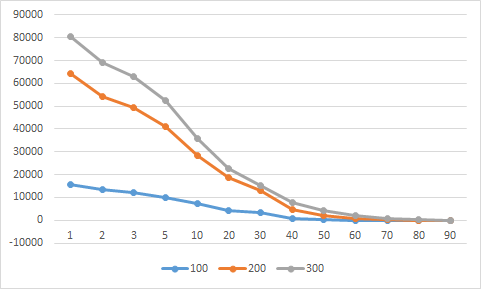
\includegraphics[scale=1]{imagenes/Experimental/DiferenciasGACEP_GRASP.png}
        \caption{Gráfica asociada a la tabla \ref{DiferenciasGACEP_GRASP}}
        \label{fig:DiferenciasGACEP}
\end{figure}

\section{Operador de Cruce Intensivo}

La siguiente idea a seguir tiene que ver de nuevo con la explotación de las características de las mejores soluciones. 
Anteriormente se propuso introducir una modificación para mejorar la explotación en el propio operador de reparación y en la mutación; en este caso, se pretende introducir este operador en el propio operador de cruce directamente. 

Esta modificación se basa en que las soluciones hijas heredarán una mayor cantidad de genes del mejor de los dos padres. 
La motivación de este cambio es la generación de nuevas soluciones muy parecidas a las buenas que ya forman parte de la población, con lo que hay una mayor probabilidad de que se sigan desarrollando las soluciones en ese ámbito. 

Para este trabajo probaremos con varios porcentajes de elementos que deben ser pertenecientes al mejor padre: 50\%, 60\%, 70\% y 80\%, para decidir cuál sería la mejor proporción. 
Téngase en cuenta que elegir el 50\% de los genes del mejor padre no tiene por qué tener el mismo resultado que el cruce uniforme que estamos actualmente realizando; ya que la primera opción permite que ambos hijos tengan genes en común (que provengan del mismo padre), mientras que para la segunda opción eso es imposible. 

Adicionalmente, consideraremos también dos posibilidades mayores: el utilizar GRASP de nuevo para este tipo de cruce o no. 
Por ello, se calculan todos los resultados posibles y se comparan entre sí para determinar cuál es la mejor opción, la cual compararemos posteriormente con nuestro GACEP con GRASP.

\subsection{Utilizando GRASP}

La lógica de utilizar GRASP para el cruce intensivo es la misma que para el cruce uniforme, la utilizaremos en el operador de reparación tras generar los hijos resultantes de dicho cruce. 

Dicho esto, podemos ver en la gráfica \ref{fig:GACEPcGRASP} el \textit{ranking} de los distintos porcentajes asociados al operador de cruce.

\begin{figure}[h]
		\centering
		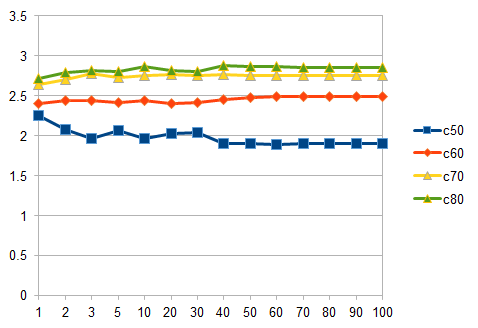
\includegraphics[scale=1]{imagenes/Experimental/GACEPcGRASP.png}
        \caption{Comparación de los resultados de los distintos porcentajes de cruce intensivo en GACEP+GRASP}
        \label{fig:GACEPcGRASP}
\end{figure}

\subsection{Sin utilizar GRASP}

En la gráfica \ref{fig:GACEPcwoGRASP} podemos apreciar el \textit{ranking} de los distintos porcentajes asociados al operador de cruce.

\begin{figure}[h]
		\centering
		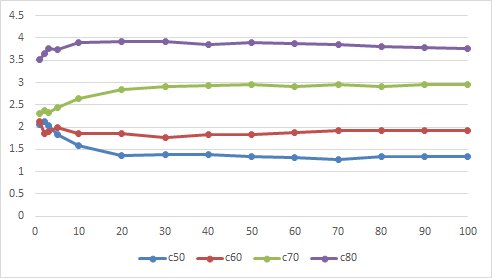
\includegraphics[scale=1]{imagenes/Experimental/GACEPcwoGRASP.png}
        \caption{Comparación de los resultados de los distintos porcentajes de cruce intensivo en GACEP}
        \label{fig:GACEPcwoGRASP}
\end{figure}

\section{Estudio de la diversidad}



\section{Incrementando la diversidad (con nuevo reemplazo)}



\section{Tablas de prueba}

































\newpage
\newpage
\newpage
\newpage
Adicionalmente, como se ha comentado antes, cada algoritmo requiere de sus propios parámetros. 
Aunque explicaremos en más profundidad cada algoritmo en los siguientes capítulos, es necesario que establezcamos ahora cuáles son dichos parámetros y qué valores se han utilizado. 
Para ello, primero vamos a resumir en la siguiente tabla (\ref{table:Parametros}) qué parámetros usa cada algoritmo y después explicaremos qué es cada uno y qué valor tienen asignado.

\begin{table}[H]
\label{table:Parametros}
\caption{Parámetros utilizados por cada algoritmo}
\begin{tabular}{|l|l|l|l|l|}
\hline
\rowcolor[HTML]{F7EAC7} 
Algoritmo          & EvaluacionMAX & Semilla     & Nº Elementos & Probabilidad mutación \\ \hline
\rowcolor[HTML]{DAE8FC} 
\textbf{Random}    & \textbf{Sí}   & \textbf{Sí} & No           & No                    \\ \hline
\rowcolor[HTML]{DDFDFF} 
\textbf{AGEU}      & \textbf{Sí}   & \textbf{Sí} & \textbf{Sí}  & \textbf{Sí}           \\ \hline
\rowcolor[HTML]{DAE8FC} 
\textbf{GACEP}     & \textbf{Sí}   & \textbf{Sí} & \textbf{Sí}  & \textbf{Sí}           \\ \hline
\rowcolor[HTML]{DDFDFF} 
\textbf{CHC}       & \textbf{Sí}   & \textbf{Sí} & \textbf{Sí}  & No                    \\ \hline
\rowcolor[HTML]{DAE8FC} 
\textbf{GACEPCHC}  & \textbf{Sí}   & \textbf{Sí} & \textbf{Sí}  & \textbf{Sí}           \\ \hline
\rowcolor[HTML]{DDFDFF} 
\textbf{GACEP3103} & \textbf{Sí}   & \textbf{Sí} & \textbf{Sí}  & \textbf{Sí}           \\ \hline
\end{tabular}
\end{table}

\begin{itemize}
	\item \texttt{EvaluacionMAX}: Es el número de evaluaciones máximas para dicho algoritmo. 
Su valor será el de \texttt{NEVALUACIONESMAX}.
	\item \texttt{Semilla}: Como se ha indicado anteriormente, es necesario establecer una semilla de aleatoriedad en cada ejecución del algoritmo. 
Por lo tanto, el valor de este parámetro será el de la semilla generada por \texttt{INITSEED}. 
	\item \texttt{Nº Elementos}: Número de soluciones que va a constituir una población. 
Es necesario tener una población pequeña con el fin de utilizar el menor número de evaluaciones posible, pero suficiente como para poder trabajar con cierto margen. 
Por lo tanto, estableceremos el tamaño de población a 10. 
	\item \texttt{Probabilidad mutación}: En algunos algoritmos intentaremos modificar un poco alguna solución en cada iteración. 
Este valor establece el porcentaje de soluciones que la población que mutará. 
Genéricamente este valor suele ser del 0.1, por lo que también lo utilizaremos en nuestro problema. 
Correspondería que solo mutaría una solución de la población por cada generación. 
\end{itemize}



% Please add the following required packages to your document preamble:
% \usepackage[table,xcdraw]{xcolor}
% If you use beamer only pass "xcolor=table" option, i.e. \documentclass[xcolor=table]{beamer}
\begin{table}[]
\begin{tabular}{r|
>{\columncolor[HTML]{D3FFB6}}r |r|}
\cline{2-3}
\multicolumn{1}{l|}{}                             & \multicolumn{1}{l|}{\cellcolor[HTML]{FFFFC7}GACEPwGRASP} & \multicolumn{1}{l|}{\cellcolor[HTML]{FFFFC7}GACEPwoGRASP} \\ \hline
\multicolumn{1}{|r|}{\cellcolor[HTML]{FCE6AB}1}   & \textbf{1.309278}                                        & 1.690722                                                  \\ \hline
\multicolumn{1}{|r|}{\cellcolor[HTML]{FCE6AB}2}   & \textbf{1.154639}                                        & 1.845361                                                  \\ \hline
\multicolumn{1}{|r|}{\cellcolor[HTML]{FCE6AB}3}   & \textbf{1.185567}                                        & 1.814433                                                  \\ \hline
\multicolumn{1}{|r|}{\cellcolor[HTML]{FCE6AB}5}   & \textbf{1.154639}                                        & 1.845361                                                  \\ \hline
\multicolumn{1}{|r|}{\cellcolor[HTML]{FCE6AB}10}  & \textbf{1.051546}                                        & 1.948454                                                  \\ \hline
\multicolumn{1}{|r|}{\cellcolor[HTML]{FCE6AB}20}  & \textbf{1.092784}                                        & 1.907216                                                  \\ \hline
\multicolumn{1}{|r|}{\cellcolor[HTML]{FCE6AB}30}  & \textbf{1.123711}                                        & 1.876289                                                  \\ \hline
\multicolumn{1}{|r|}{\cellcolor[HTML]{FCE6AB}40}  & \textbf{1.061856}                                        & 1.938144                                                  \\ \hline
\multicolumn{1}{|r|}{\cellcolor[HTML]{FCE6AB}50}  & \textbf{1.082474}                                        & 1.917526                                                  \\ \hline
\multicolumn{1}{|r|}{\cellcolor[HTML]{FCE6AB}60}  & \textbf{1.072165}                                        & 1.927835                                                  \\ \hline
\multicolumn{1}{|r|}{\cellcolor[HTML]{FCE6AB}70}  & \textbf{1.103093}                                        & 1.896907                                                  \\ \hline
\multicolumn{1}{|r|}{\cellcolor[HTML]{FCE6AB}80}  & \textbf{1.103093}                                        & 1.896907                                                  \\ \hline
\multicolumn{1}{|r|}{\cellcolor[HTML]{FCE6AB}90}  & \textbf{1.103093}                                        & 1.896907                                                  \\ \hline
\multicolumn{1}{|r|}{\cellcolor[HTML]{FCE6AB}100} & \textbf{1.103093}                                        & 1.896907                                                  \\ \hline
\end{tabular}
\caption{Solo Ranking}
\end{table}

% Please add the following required packages to your document preamble:
% \usepackage[table,xcdraw]{xcolor}
% If you use beamer only pass "xcolor=table" option, i.e. \documentclass[xcolor=table]{beamer}
\begin{table}[]
\begin{tabular}{l|r|r|}
\cline{2-3}
                                                   & \multicolumn{1}{l|}{\cellcolor[HTML]{FFFFC7}GACEPwGRASP} & \multicolumn{1}{l|}{\cellcolor[HTML]{FFFFC7}GACEPwoGRASP} \\ \hline
\multicolumn{1}{|l|}{\cellcolor[HTML]{FCE6AB}F01}  & 203870                                                   & \cellcolor[HTML]{D3FFB6}\textbf{203917}                   \\ \hline
\multicolumn{1}{|l|}{\cellcolor[HTML]{FCE6AB}F02}  & \cellcolor[HTML]{D3FFB6}\textbf{88229.5}                 & 86893.8                                                   \\ \hline
\multicolumn{1}{|l|}{\cellcolor[HTML]{FCE6AB}F03}  & \cellcolor[HTML]{D3FFB6}\textbf{202940}                  & 202056                                                    \\ \hline
\multicolumn{1}{|l|}{\cellcolor[HTML]{FCE6AB}F04}  & \cellcolor[HTML]{D3FFB6}\textbf{235610}                  & 234528                                                    \\ \hline
\multicolumn{1}{|l|}{\cellcolor[HTML]{FCE6AB}F05}  & 238439                                                   & \cellcolor[HTML]{D3FFB6}\textbf{238931}                   \\ \hline
\multicolumn{1}{|l|}{\cellcolor[HTML]{FCE6AB}F06}  & \cellcolor[HTML]{D3FFB6}\textbf{81325.7}                 & 78698.4                                                   \\ \hline
\multicolumn{1}{|l|}{\cellcolor[HTML]{FCE6AB}F07}  & \cellcolor[HTML]{D3FFB6}\textbf{10867.2}                 & 10611.2                                                   \\ \hline
\multicolumn{1}{|l|}{\cellcolor[HTML]{FCE6AB}F08}  & \cellcolor[HTML]{D3FFB6}\textbf{67669.3}                 & 67007.1                                                   \\ \hline
\multicolumn{1}{|l|}{\cellcolor[HTML]{FCE6AB}F09}  & 239982                                                   & \cellcolor[HTML]{D3FFB6}\textbf{241977}                   \\ \hline
\multicolumn{1}{|l|}{\cellcolor[HTML]{FCE6AB}F10}  & \cellcolor[HTML]{D3FFB6}\textbf{26642.1}                 & 26107.5                                                   \\ \hline
\multicolumn{1}{|l|}{\cellcolor[HTML]{FCE6AB}F11}  & \cellcolor[HTML]{D3FFB6}\textbf{20217.6}                 & 20195.7                                                   \\ \hline
\multicolumn{1}{|l|}{\cellcolor[HTML]{FCE6AB}F12}  & \cellcolor[HTML]{D3FFB6}\textbf{58173.8}                 & 58108.8                                                   \\ \hline
\multicolumn{1}{|l|}{\cellcolor[HTML]{FCE6AB}F13}  & \cellcolor[HTML]{D3FFB6}\textbf{3967.14}                 & 3841.06                                                   \\ \hline
\multicolumn{1}{|l|}{\cellcolor[HTML]{FCE6AB}F14}  & \cellcolor[HTML]{D3FFB6}\textbf{53183.3}                 & 52534.5                                                   \\ \hline
\multicolumn{1}{|l|}{\cellcolor[HTML]{FCE6AB}F15}  & 62310.9                                                  & \cellcolor[HTML]{D3FFB6}\textbf{62661.5}                  \\ \hline
\multicolumn{1}{|l|}{\cellcolor[HTML]{FCE6AB}F16}  & \cellcolor[HTML]{D3FFB6}\textbf{38963}                   & 38120.5                                                   \\ \hline
\multicolumn{1}{|l|}{\cellcolor[HTML]{FCE6AB}F17}  & \cellcolor[HTML]{D3FFB6}\textbf{15641.2}                 & 15454.7                                                   \\ \hline
\multicolumn{1}{|l|}{\cellcolor[HTML]{FCE6AB}F18}  & \cellcolor[HTML]{D3FFB6}\textbf{22181.6}                 & 21423.6                                                   \\ \hline
\multicolumn{1}{|l|}{\cellcolor[HTML]{FCE6AB}F19}  & \cellcolor[HTML]{D3FFB6}\textbf{37575.9}                 & 36782.8                                                   \\ \hline
\multicolumn{1}{|l|}{\cellcolor[HTML]{FCE6AB}F20}  & 94259.5                                                  & \cellcolor[HTML]{D3FFB6}\textbf{94302.4}                  \\ \hline
\multicolumn{1}{|l|}{\cellcolor[HTML]{FCE6AB}F21}  & \cellcolor[HTML]{D3FFB6}\textbf{89232.8}                 & 88189.9                                                   \\ \hline
\multicolumn{1}{|l|}{\cellcolor[HTML]{FCE6AB}F22}  & \cellcolor[HTML]{D3FFB6}\textbf{110642}                  & 108332                                                    \\ \hline
\multicolumn{1}{|l|}{\cellcolor[HTML]{FCE6AB}F23}  & \cellcolor[HTML]{D3FFB6}\textbf{37247.4}                 & 36961.9                                                   \\ \hline
\multicolumn{1}{|l|}{\cellcolor[HTML]{FCE6AB}F24}  & 110026                                                   & \cellcolor[HTML]{D3FFB6}\textbf{110489}                   \\ \hline
\multicolumn{1}{|l|}{\cellcolor[HTML]{FCE6AB}F25}  & \cellcolor[HTML]{D3FFB6}\textbf{60821.5}                 & 57749                                                     \\ \hline
\multicolumn{1}{|l|}{\cellcolor[HTML]{FCE6AB}F26}  & \cellcolor[HTML]{D3FFB6}\textbf{18066.4}                 & 17239.7                                                   \\ \hline
\multicolumn{1}{|l|}{\cellcolor[HTML]{FCE6AB}F27}  & \cellcolor[HTML]{D3FFB6}\textbf{55937.8}                 & 55209.6                                                   \\ \hline
\multicolumn{1}{|l|}{\cellcolor[HTML]{FCE6AB}F28}  & \cellcolor[HTML]{D3FFB6}\textbf{58848.7}                 & 57800.7                                                   \\ \hline
\multicolumn{1}{|l|}{\cellcolor[HTML]{FCE6AB}F29}  & \cellcolor[HTML]{D3FFB6}\textbf{73569.8}                 & 72183.1                                                   \\ \hline
\multicolumn{1}{|l|}{\cellcolor[HTML]{FCE6AB}F30}  & \cellcolor[HTML]{D3FFB6}\textbf{151250}                  & 151073                                                    \\ \hline
\multicolumn{1}{|l|}{\cellcolor[HTML]{FCE6AB}F31}  & 191323                                                   & \cellcolor[HTML]{D3FFB6}\textbf{191744}                   \\ \hline
\multicolumn{1}{|l|}{\cellcolor[HTML]{FCE6AB}F32}  & \cellcolor[HTML]{D3FFB6}\textbf{104160}                  & 101933                                                    \\ \hline
\multicolumn{1}{|l|}{\cellcolor[HTML]{FCE6AB}F33}  & \cellcolor[HTML]{D3FFB6}\textbf{66522.7}                 & 65749.4                                                   \\ \hline
\multicolumn{1}{|l|}{\cellcolor[HTML]{FCE6AB}F34}  & \cellcolor[HTML]{D3FFB6}\textbf{80481.7}                 & 78826.7                                                   \\ \hline
\multicolumn{1}{|l|}{\cellcolor[HTML]{FCE6AB}F35}  & \cellcolor[HTML]{D3FFB6}\textbf{31122.7}                 & 30323.9                                                   \\ \hline
\multicolumn{1}{|l|}{\cellcolor[HTML]{FCE6AB}F36}  & \cellcolor[HTML]{D3FFB6}\textbf{153157}                  & 150580                                                    \\ \hline
\multicolumn{1}{|l|}{\cellcolor[HTML]{FCE6AB}F37}  & \cellcolor[HTML]{D3FFB6}\textbf{120369}                  & 118139                                                    \\ \hline
\multicolumn{1}{|l|}{\cellcolor[HTML]{FCE6AB}F38}  & \cellcolor[HTML]{D3FFB6}\textbf{21816.6}                 & 21744.5                                                   \\ \hline
\multicolumn{1}{|l|}{\cellcolor[HTML]{FCE6AB}F39}  & \cellcolor[HTML]{D3FFB6}\textbf{112427}                  & 111748                                                    \\ \hline
\multicolumn{1}{|l|}{\cellcolor[HTML]{FCE6AB}F40}  & \cellcolor[HTML]{D3FFB6}\textbf{379570}                  & 371906                                                    \\ \hline
\multicolumn{1}{|l|}{\cellcolor[HTML]{FCE6AB}F41}  & 958934                                                   & \cellcolor[HTML]{D3FFB6}\textbf{960695}                   \\ \hline
\multicolumn{1}{|l|}{\cellcolor[HTML]{FCE6AB}F42}  & \cellcolor[HTML]{D3FFB6}\textbf{315558}                  & 310368                                                    \\ \hline
\multicolumn{1}{|l|}{\cellcolor[HTML]{FCE6AB}F43}  & \cellcolor[HTML]{D3FFB6}\textbf{32375.5}                 & 31956                                                     \\ \hline
\multicolumn{1}{|l|}{\cellcolor[HTML]{FCE6AB}F44}  & 106229                                                   & \cellcolor[HTML]{D3FFB6}\textbf{107874}                   \\ \hline
\multicolumn{1}{|l|}{\cellcolor[HTML]{FCE6AB}F45}  & \cellcolor[HTML]{D3FFB6}\textbf{813622}                  & 804278                                                    \\ \hline
\multicolumn{1}{|l|}{\cellcolor[HTML]{FCE6AB}F46}  & \cellcolor[HTML]{D3FFB6}\textbf{44144.1}                 & 43930.7                                                   \\ \hline
\multicolumn{1}{|l|}{\cellcolor[HTML]{FCE6AB}F47}  & \cellcolor[HTML]{D3FFB6}\textbf{726019}                  & 711466                                                    \\ \hline
\multicolumn{1}{|l|}{\cellcolor[HTML]{FCE6AB}F48}  & \cellcolor[HTML]{D3FFB6}\textbf{813949}                  & 805644                                                    \\ \hline
\multicolumn{1}{|l|}{\cellcolor[HTML]{FCE6AB}F49}  & \cellcolor[HTML]{D3FFB6}\textbf{653176}                  & 639675                                                    \\ \hline
\multicolumn{1}{|l|}{\cellcolor[HTML]{FCE6AB}F50}  & \cellcolor[HTML]{D3FFB6}\textbf{50543}                   & 49255.1                                                   \\ \hline
\multicolumn{1}{|l|}{\cellcolor[HTML]{FCE6AB}F51}  & \cellcolor[HTML]{D3FFB6}\textbf{211429}                  & 206394                                                    \\ \hline
\multicolumn{1}{|l|}{\cellcolor[HTML]{FCE6AB}F52}  & \cellcolor[HTML]{D3FFB6}\textbf{244518}                  & 243532                                                    \\ \hline
\multicolumn{1}{|l|}{\cellcolor[HTML]{FCE6AB}F53}  & \cellcolor[HTML]{D3FFB6}\textbf{227361}                  & 226204                                                    \\ \hline
\multicolumn{1}{|l|}{\cellcolor[HTML]{FCE6AB}F54}  & \cellcolor[HTML]{D3FFB6}\textbf{193634}                  & 189500                                                    \\ \hline
\multicolumn{1}{|l|}{\cellcolor[HTML]{FCE6AB}F55}  & \cellcolor[HTML]{D3FFB6}\textbf{81477.9}                 & 78811.9                                                   \\ \hline
\multicolumn{1}{|l|}{\cellcolor[HTML]{FCE6AB}F56}  & \cellcolor[HTML]{D3FFB6}\textbf{61504}                   & 59037                                                     \\ \hline
\multicolumn{1}{|l|}{\cellcolor[HTML]{FCE6AB}F57}  & \cellcolor[HTML]{D3FFB6}\textbf{150655}                  & 146471                                                    \\ \hline
\multicolumn{1}{|l|}{\cellcolor[HTML]{FCE6AB}F58}  & \cellcolor[HTML]{D3FFB6}\textbf{51459}                   & 49706.3                                                   \\ \hline
\multicolumn{1}{|l|}{\cellcolor[HTML]{FCE6AB}F59}  & \cellcolor[HTML]{D3FFB6}\textbf{287285}                  & 283170                                                    \\ \hline
\multicolumn{1}{|l|}{\cellcolor[HTML]{FCE6AB}F60}  & \cellcolor[HTML]{D3FFB6}\textbf{383329}                  & 374933                                                    \\ \hline
\multicolumn{1}{|l|}{\cellcolor[HTML]{FCE6AB}F61}  & \cellcolor[HTML]{D3FFB6}\textbf{214848}                  & 205342                                                    \\ \hline
\multicolumn{1}{|l|}{\cellcolor[HTML]{FCE6AB}F62}  & \cellcolor[HTML]{D3FFB6}\textbf{225192}                  & 219207                                                    \\ \hline
\multicolumn{1}{|l|}{\cellcolor[HTML]{FCE6AB}F63}  & \cellcolor[HTML]{D3FFB6}\textbf{225684}                  & 220104                                                    \\ \hline
\multicolumn{1}{|l|}{\cellcolor[HTML]{FCE6AB}F64}  & 489291                                                   & \cellcolor[HTML]{D3FFB6}\textbf{490903}                   \\ \hline
\multicolumn{1}{|l|}{\cellcolor[HTML]{FCE6AB}F65}  & \cellcolor[HTML]{D3FFB6}\textbf{440828}                  & 439020                                                    \\ \hline
\multicolumn{1}{|l|}{\cellcolor[HTML]{FCE6AB}F66}  & \cellcolor[HTML]{D3FFB6}\textbf{220101}                  & 214588                                                    \\ \hline
\multicolumn{1}{|l|}{\cellcolor[HTML]{FCE6AB}F67}  & \cellcolor[HTML]{D3FFB6}\textbf{324902}                  & 318589                                                    \\ \hline
\multicolumn{1}{|l|}{\cellcolor[HTML]{FCE6AB}F68}  & \cellcolor[HTML]{D3FFB6}\textbf{110572}                  & 108423                                                    \\ \hline
\multicolumn{1}{|l|}{\cellcolor[HTML]{FCE6AB}F69}  & \cellcolor[HTML]{D3FFB6}\textbf{150784}                  & 148614                                                    \\ \hline
\multicolumn{1}{|l|}{\cellcolor[HTML]{FCE6AB}F70}  & \cellcolor[HTML]{D3FFB6}\textbf{452607}                  & 445441                                                    \\ \hline
\multicolumn{1}{|l|}{\cellcolor[HTML]{FCE6AB}F71}  & \cellcolor[HTML]{D3FFB6}\textbf{281795}                  & 277919                                                    \\ \hline
\multicolumn{1}{|l|}{\cellcolor[HTML]{FCE6AB}F72}  & \cellcolor[HTML]{D3FFB6}\textbf{66610.6}                 & 65806.9                                                   \\ \hline
\multicolumn{1}{|l|}{\cellcolor[HTML]{FCE6AB}F73}  & \cellcolor[HTML]{D3FFB6}\textbf{133906}                  & 133560                                                    \\ \hline
\multicolumn{1}{|l|}{\cellcolor[HTML]{FCE6AB}F74}  & \cellcolor[HTML]{D3FFB6}\textbf{146870}                  & 144762                                                    \\ \hline
\multicolumn{1}{|l|}{\cellcolor[HTML]{FCE6AB}F75}  & \cellcolor[HTML]{D3FFB6}\textbf{234757}                  & 232794                                                    \\ \hline
\multicolumn{1}{|l|}{\cellcolor[HTML]{FCE6AB}F76}  & \cellcolor[HTML]{D3FFB6}\textbf{275504}                  & 269788                                                    \\ \hline
\multicolumn{1}{|l|}{\cellcolor[HTML]{FCE6AB}F77}  & \cellcolor[HTML]{D3FFB6}\textbf{620630}                  & 616128                                                    \\ \hline
\multicolumn{1}{|l|}{\cellcolor[HTML]{FCE6AB}F78}  & \cellcolor[HTML]{D3FFB6}\textbf{534844}                  & 525471                                                    \\ \hline
\multicolumn{1}{|l|}{\cellcolor[HTML]{FCE6AB}F79}  & \cellcolor[HTML]{D3FFB6}\textbf{379471}                  & 370202                                                    \\ \hline
\multicolumn{1}{|l|}{\cellcolor[HTML]{FCE6AB}F80}  & \cellcolor[HTML]{D3FFB6}\textbf{30802.7}                 & 30668.8                                                   \\ \hline
\multicolumn{1}{|l|}{\cellcolor[HTML]{FCE6AB}F81}  & \cellcolor[HTML]{D3FFB6}\textbf{269072}                  & 261697                                                    \\ \hline
\multicolumn{1}{|l|}{\cellcolor[HTML]{FCE6AB}F82}  & \cellcolor[HTML]{D3FFB6}\textbf{453902}                  & 441509                                                    \\ \hline
\multicolumn{1}{|l|}{\cellcolor[HTML]{FCE6AB}F83}  & \cellcolor[HTML]{D3FFB6}\textbf{15967.4}                 & 15628.8                                                   \\ \hline
\multicolumn{1}{|l|}{\cellcolor[HTML]{FCE6AB}F84}  & \cellcolor[HTML]{D3FFB6}\textbf{253405}                  & 245342                                                    \\ \hline
\multicolumn{1}{|l|}{\cellcolor[HTML]{FCE6AB}F85}  & \cellcolor[HTML]{D3FFB6}\textbf{494802}                  & 487566                                                    \\ \hline
\multicolumn{1}{|l|}{\cellcolor[HTML]{FCE6AB}F86}  & \cellcolor[HTML]{D3FFB6}\textbf{9783.9}                  & 9749.8                                                    \\ \hline
\multicolumn{1}{|l|}{\cellcolor[HTML]{FCE6AB}F87}  & \cellcolor[HTML]{D3FFB6}\textbf{237551}                  & 226145                                                    \\ \hline
\multicolumn{1}{|l|}{\cellcolor[HTML]{FCE6AB}F88}  & \cellcolor[HTML]{D3FFB6}\textbf{1017990}                 & 1009100                                                   \\ \hline
\multicolumn{1}{|l|}{\cellcolor[HTML]{FCE6AB}F89}  & \cellcolor[HTML]{D3FFB6}\textbf{483693}                  & 469319                                                    \\ \hline
\multicolumn{1}{|l|}{\cellcolor[HTML]{FCE6AB}F90}  & \cellcolor[HTML]{D3FFB6}\textbf{110079}                  & 105789                                                    \\ \hline
\multicolumn{1}{|l|}{\cellcolor[HTML]{FCE6AB}F91}  & \cellcolor[HTML]{D3FFB6}\textbf{890216}                  & 873907                                                    \\ \hline
\multicolumn{1}{|l|}{\cellcolor[HTML]{FCE6AB}F92}  & \cellcolor[HTML]{D3FFB6}\textbf{310174}                  & 295377                                                    \\ \hline
\multicolumn{1}{|l|}{\cellcolor[HTML]{FCE6AB}F93}  & \cellcolor[HTML]{D3FFB6}\textbf{722245}                  & 706744                                                    \\ \hline
\multicolumn{1}{|l|}{\cellcolor[HTML]{FCE6AB}F94}  & \cellcolor[HTML]{D3FFB6}\textbf{738970}                  & 719059                                                    \\ \hline
\multicolumn{1}{|l|}{\cellcolor[HTML]{FCE6AB}F95}  & \cellcolor[HTML]{D3FFB6}\textbf{46951.9}                 & 46737.7                                                   \\ \hline
\multicolumn{1}{|l|}{\cellcolor[HTML]{FCE6AB}F96}  & \cellcolor[HTML]{D3FFB6}\textbf{770539}                  & 751434                                                    \\ \hline
\multicolumn{1}{|l|}{\cellcolor[HTML]{FCE6AB}F97}  & \cellcolor[HTML]{D3FFB6}\textbf{766150}                  & 752530                                                    \\ \hline
\multicolumn{1}{|l|}{\cellcolor[HTML]{FFFFC7}Best} & \multicolumn{1}{c|}{\cellcolor[HTML]{D3FFB6}\textbf{87}} & \multicolumn{1}{c|}{10}                                   \\ \hline
\end{tabular}
\caption{Solo valores}
\end{table}

% Please add the following required packages to your document preamble:
% \usepackage[table,xcdraw]{xcolor}
% If you use beamer only pass "xcolor=table" option, i.e. \documentclass[xcolor=table]{beamer}
\begin{table}[]
\begin{tabular}{lrr|}
\cline{2-3}
\multicolumn{1}{l|}{}                             & \multicolumn{1}{l|}{\cellcolor[HTML]{FFFFC7}GACEPwGRASP}      & \multicolumn{1}{l|}{\cellcolor[HTML]{FFFFC7}GACEPwoGRASP} \\ \hline
\multicolumn{1}{|l|}{\cellcolor[HTML]{FCE6AB}F01} & \multicolumn{1}{r|}{203870}                                   & \cellcolor[HTML]{D3FFB6}\textbf{203917}                   \\ \hline
\multicolumn{1}{|l|}{\cellcolor[HTML]{FCE6AB}F02} & \multicolumn{1}{r|}{\cellcolor[HTML]{D3FFB6}\textbf{88229.5}} & 86893.8                                                   \\ \hline
\multicolumn{1}{|l|}{\cellcolor[HTML]{FCE6AB}F03} & \multicolumn{1}{r|}{\cellcolor[HTML]{D3FFB6}\textbf{202940}}  & 202056                                                    \\ \hline
\multicolumn{1}{|l|}{\cellcolor[HTML]{FCE6AB}F04} & \multicolumn{1}{r|}{\cellcolor[HTML]{D3FFB6}\textbf{235610}}  & 234528                                                    \\ \hline
\multicolumn{1}{|l|}{\cellcolor[HTML]{FCE6AB}F05} & \multicolumn{1}{r|}{238439}                                   & \cellcolor[HTML]{D3FFB6}\textbf{238931}                   \\ \hline
\multicolumn{1}{|l|}{\cellcolor[HTML]{FCE6AB}F06} & \multicolumn{1}{r|}{\cellcolor[HTML]{D3FFB6}\textbf{81325.7}} & 78698.4                                                   \\ \hline
\multicolumn{1}{|l|}{\cellcolor[HTML]{FCE6AB}F07} & \multicolumn{1}{r|}{\cellcolor[HTML]{D3FFB6}\textbf{10867.2}} & 10611.2                                                   \\ \hline
\multicolumn{1}{|l|}{\cellcolor[HTML]{FCE6AB}F08} & \multicolumn{1}{r|}{\cellcolor[HTML]{D3FFB6}\textbf{67669.3}} & 67007.1                                                   \\ \hline
\multicolumn{1}{|l|}{\cellcolor[HTML]{FCE6AB}F09} & \multicolumn{1}{r|}{239982}                                   & \cellcolor[HTML]{D3FFB6}\textbf{241977}                   \\ \hline
\multicolumn{1}{|l|}{\cellcolor[HTML]{FCE6AB}F10} & \multicolumn{1}{r|}{\cellcolor[HTML]{D3FFB6}\textbf{26642.1}} & 26107.5                                                   \\ \hline
\multicolumn{1}{|l|}{\cellcolor[HTML]{FCE6AB}F11} & \multicolumn{1}{r|}{\cellcolor[HTML]{D3FFB6}\textbf{20217.6}} & 20195.7                                                   \\ \hline
\multicolumn{1}{|l|}{\cellcolor[HTML]{FCE6AB}F12} & \multicolumn{1}{r|}{\cellcolor[HTML]{D3FFB6}\textbf{58173.8}} & 58108.8                                                   \\ \hline
\multicolumn{1}{|l|}{\cellcolor[HTML]{FCE6AB}F13} & \multicolumn{1}{r|}{\cellcolor[HTML]{D3FFB6}\textbf{3967.14}} & 3841.06                                                   \\ \hline
\multicolumn{1}{|l|}{\cellcolor[HTML]{FCE6AB}F14} & \multicolumn{1}{r|}{\cellcolor[HTML]{D3FFB6}\textbf{53183.3}} & 52534.5                                                   \\ \hline
\multicolumn{1}{|l|}{\cellcolor[HTML]{FCE6AB}F15} & \multicolumn{1}{r|}{62310.9}                                  & \cellcolor[HTML]{D3FFB6}\textbf{62661.5}                  \\ \hline
\multicolumn{1}{|l|}{\cellcolor[HTML]{FCE6AB}F16} & \multicolumn{1}{r|}{\cellcolor[HTML]{D3FFB6}\textbf{38963}}   & 38120.5                                                   \\ \hline
\multicolumn{1}{|l|}{\cellcolor[HTML]{FCE6AB}F17} & \multicolumn{1}{r|}{\cellcolor[HTML]{D3FFB6}\textbf{15641.2}} & 15454.7                                                   \\ \hline
\multicolumn{1}{|l|}{\cellcolor[HTML]{FCE6AB}F18} & \multicolumn{1}{r|}{\cellcolor[HTML]{D3FFB6}\textbf{22181.6}} & 21423.6                                                   \\ \hline
\multicolumn{1}{|l|}{\cellcolor[HTML]{FCE6AB}F19} & \multicolumn{1}{r|}{\cellcolor[HTML]{D3FFB6}\textbf{37575.9}} & 36782.8                                                   \\ \hline
\multicolumn{1}{|l|}{\cellcolor[HTML]{FCE6AB}F20} & \multicolumn{1}{r|}{94259.5}                                  & \cellcolor[HTML]{D3FFB6}\textbf{94302.4}                  \\ \hline
\multicolumn{1}{|l|}{\cellcolor[HTML]{FCE6AB}F21} & \multicolumn{1}{r|}{\cellcolor[HTML]{D3FFB6}\textbf{89232.8}} & 88189.9                                                   \\ \hline
\multicolumn{1}{|l|}{\cellcolor[HTML]{FCE6AB}F22} & \multicolumn{1}{r|}{\cellcolor[HTML]{D3FFB6}\textbf{110642}}  & 108332                                                    \\ \hline
\multicolumn{1}{|l|}{\cellcolor[HTML]{FCE6AB}F23} & \multicolumn{1}{r|}{\cellcolor[HTML]{D3FFB6}\textbf{37247.4}} & 36961.9                                                   \\ \hline
\multicolumn{1}{|l|}{\cellcolor[HTML]{FCE6AB}F24} & \multicolumn{1}{r|}{110026}                                   & \cellcolor[HTML]{D3FFB6}\textbf{110489}                   \\ \hline
\multicolumn{1}{|l|}{\cellcolor[HTML]{FCE6AB}F25} & \multicolumn{1}{r|}{\cellcolor[HTML]{D3FFB6}\textbf{60821.5}} & 57749                                                     \\ \hline
\multicolumn{1}{|l|}{\cellcolor[HTML]{FCE6AB}F26} & \multicolumn{1}{r|}{\cellcolor[HTML]{D3FFB6}\textbf{18066.4}} & 17239.7                                                   \\ \hline
\multicolumn{1}{|l|}{\cellcolor[HTML]{FCE6AB}F27} & \multicolumn{1}{r|}{\cellcolor[HTML]{D3FFB6}\textbf{55937.8}} & 55209.6                                                   \\ \hline
\multicolumn{1}{|l|}{\cellcolor[HTML]{FCE6AB}F28} & \multicolumn{1}{r|}{\cellcolor[HTML]{D3FFB6}\textbf{58848.7}} & 57800.7                                                   \\ \hline
\multicolumn{1}{|l|}{\cellcolor[HTML]{FCE6AB}F29} & \multicolumn{1}{r|}{\cellcolor[HTML]{D3FFB6}\textbf{73569.8}} & 72183.1                                                   \\ \hline
\multicolumn{1}{|l|}{\cellcolor[HTML]{FCE6AB}F30} & \multicolumn{1}{r|}{\cellcolor[HTML]{D3FFB6}\textbf{151250}}  & 151073                                                    \\ \hline
\multicolumn{1}{|l|}{\cellcolor[HTML]{FCE6AB}F31} & \multicolumn{1}{r|}{191323}                                   & \cellcolor[HTML]{D3FFB6}\textbf{191744}                   \\ \hline
\multicolumn{1}{|l|}{\cellcolor[HTML]{FCE6AB}F32} & \multicolumn{1}{r|}{\cellcolor[HTML]{D3FFB6}\textbf{104160}}  & 101933                                                    \\ \hline
\multicolumn{1}{|l|}{\cellcolor[HTML]{FCE6AB}F33} & \multicolumn{1}{r|}{\cellcolor[HTML]{D3FFB6}\textbf{66522.7}} & 65749.4                                                   \\ \hline
\multicolumn{1}{|l|}{\cellcolor[HTML]{FCE6AB}F34} & \multicolumn{1}{r|}{\cellcolor[HTML]{D3FFB6}\textbf{80481.7}} & 78826.7                                                   \\ \hline
\multicolumn{1}{|l|}{\cellcolor[HTML]{FCE6AB}F35} & \multicolumn{1}{r|}{\cellcolor[HTML]{D3FFB6}\textbf{31122.7}} & 30323.9                                                   \\ \hline
\multicolumn{1}{|l|}{\cellcolor[HTML]{FCE6AB}F36} & \multicolumn{1}{r|}{\cellcolor[HTML]{D3FFB6}\textbf{153157}}  & 150580                                                    \\ \hline
\multicolumn{1}{|l|}{\cellcolor[HTML]{FCE6AB}F37} & \multicolumn{1}{r|}{\cellcolor[HTML]{D3FFB6}\textbf{120369}}  & 118139                                                    \\ \hline
\multicolumn{1}{|l|}{\cellcolor[HTML]{FCE6AB}F38} & \multicolumn{1}{r|}{\cellcolor[HTML]{D3FFB6}\textbf{21816.6}} & 21744.5                                                   \\ \hline
\multicolumn{1}{|l|}{\cellcolor[HTML]{FCE6AB}F39} & \multicolumn{1}{r|}{\cellcolor[HTML]{D3FFB6}\textbf{112427}}  & 111748                                                    \\ \hline
\multicolumn{1}{|l|}{\cellcolor[HTML]{FCE6AB}F40} & \multicolumn{1}{r|}{\cellcolor[HTML]{D3FFB6}\textbf{379570}}  & 371906                                                    \\ \hline
\multicolumn{1}{|l|}{\cellcolor[HTML]{FCE6AB}F41} & \multicolumn{1}{r|}{958934}                                   & \cellcolor[HTML]{D3FFB6}\textbf{960695}                   \\ \hline
\multicolumn{1}{|l|}{\cellcolor[HTML]{FCE6AB}F42} & \multicolumn{1}{r|}{\cellcolor[HTML]{D3FFB6}\textbf{315558}}  & 310368                                                    \\ \hline
\multicolumn{1}{|l|}{\cellcolor[HTML]{FCE6AB}F43} & \multicolumn{1}{r|}{\cellcolor[HTML]{D3FFB6}\textbf{32375.5}} & 31956                                                     \\ \hline
\multicolumn{1}{|l|}{\cellcolor[HTML]{FCE6AB}F44} & \multicolumn{1}{r|}{106229}                                   & \cellcolor[HTML]{D3FFB6}\textbf{107874}                   \\ \hline
\multicolumn{1}{|l|}{\cellcolor[HTML]{FCE6AB}F45} & \multicolumn{1}{r|}{\cellcolor[HTML]{D3FFB6}\textbf{813622}}  & 804278                                                    \\ \hline
\multicolumn{1}{|l|}{\cellcolor[HTML]{FCE6AB}F46} & \multicolumn{1}{r|}{\cellcolor[HTML]{D3FFB6}\textbf{44144.1}} & 43930.7                                                   \\ \hline
\multicolumn{1}{|l|}{\cellcolor[HTML]{FCE6AB}F47} & \multicolumn{1}{r|}{\cellcolor[HTML]{D3FFB6}\textbf{726019}}  & 711466                                                    \\ \hline
\multicolumn{1}{|l|}{\cellcolor[HTML]{FCE6AB}F48} & \multicolumn{1}{r|}{\cellcolor[HTML]{D3FFB6}\textbf{813949}}  & 805644                                                    \\ \hline
\multicolumn{1}{|l|}{\cellcolor[HTML]{FCE6AB}F49} & \multicolumn{1}{r|}{\cellcolor[HTML]{D3FFB6}\textbf{653176}}  & 639675                                                    \\ \hline
\multicolumn{1}{|l|}{\cellcolor[HTML]{FCE6AB}F50} & \multicolumn{1}{r|}{\cellcolor[HTML]{D3FFB6}\textbf{50543}}   & 49255.1                                                   \\ \hline
\multicolumn{1}{|l|}{\cellcolor[HTML]{FCE6AB}F51} & \multicolumn{1}{r|}{\cellcolor[HTML]{D3FFB6}\textbf{211429}}  & 206394                                                    \\ \hline
\multicolumn{1}{|l|}{\cellcolor[HTML]{FCE6AB}F52} & \multicolumn{1}{r|}{\cellcolor[HTML]{D3FFB6}\textbf{244518}}  & 243532                                                    \\ \hline
\multicolumn{1}{|l|}{\cellcolor[HTML]{FCE6AB}F53} & \multicolumn{1}{r|}{\cellcolor[HTML]{D3FFB6}\textbf{227361}}  & 226204                                                    \\ \hline
\multicolumn{1}{|l|}{\cellcolor[HTML]{FCE6AB}F54} & \multicolumn{1}{r|}{\cellcolor[HTML]{D3FFB6}\textbf{193634}}  & 189500                                                    \\ \hline
\multicolumn{1}{|l|}{\cellcolor[HTML]{FCE6AB}F55} & \multicolumn{1}{r|}{\cellcolor[HTML]{D3FFB6}\textbf{81477.9}} & 78811.9                                                   \\ \hline
\multicolumn{1}{|l|}{\cellcolor[HTML]{FCE6AB}F56} & \multicolumn{1}{r|}{\cellcolor[HTML]{D3FFB6}\textbf{61504}}   & 59037                                                     \\ \hline
\multicolumn{1}{|l|}{\cellcolor[HTML]{FCE6AB}F57} & \multicolumn{1}{r|}{\cellcolor[HTML]{D3FFB6}\textbf{150655}}  & 146471                                                    \\ \hline
\multicolumn{1}{|l|}{\cellcolor[HTML]{FCE6AB}F58} & \multicolumn{1}{r|}{\cellcolor[HTML]{D3FFB6}\textbf{51459}}   & 49706.3                                                   \\ \hline
\multicolumn{1}{|l|}{\cellcolor[HTML]{FCE6AB}F59} & \multicolumn{1}{r|}{\cellcolor[HTML]{D3FFB6}\textbf{287285}}  & 283170                                                    \\ \hline
\multicolumn{1}{|l|}{\cellcolor[HTML]{FCE6AB}F60} & \multicolumn{1}{r|}{\cellcolor[HTML]{D3FFB6}\textbf{383329}}  & 374933                                                    \\ \hline
\multicolumn{1}{|l|}{\cellcolor[HTML]{FCE6AB}F61} & \multicolumn{1}{r|}{\cellcolor[HTML]{D3FFB6}\textbf{214848}}  & 205342                                                    \\ \hline
\multicolumn{1}{|l|}{\cellcolor[HTML]{FCE6AB}F62} & \multicolumn{1}{r|}{\cellcolor[HTML]{D3FFB6}\textbf{225192}}  & 219207                                                    \\ \hline
\multicolumn{1}{|l|}{\cellcolor[HTML]{FCE6AB}F63} & \multicolumn{1}{r|}{\cellcolor[HTML]{D3FFB6}\textbf{225684}}  & 220104                                                    \\ \hline
\multicolumn{1}{|l|}{\cellcolor[HTML]{FCE6AB}F64} & \multicolumn{1}{r|}{489291}                                   & \cellcolor[HTML]{D3FFB6}\textbf{490903}                   \\ \hline
\multicolumn{1}{|l|}{\cellcolor[HTML]{FCE6AB}F65} & \multicolumn{1}{r|}{\cellcolor[HTML]{D3FFB6}\textbf{440828}}  & 439020                                                    \\ \hline
\multicolumn{1}{|l|}{\cellcolor[HTML]{FCE6AB}F66} & \multicolumn{1}{r|}{\cellcolor[HTML]{D3FFB6}\textbf{220101}}  & 214588                                                    \\ \hline
\multicolumn{1}{|l|}{\cellcolor[HTML]{FCE6AB}F67} & \multicolumn{1}{r|}{\cellcolor[HTML]{D3FFB6}\textbf{324902}}  & 318589                                                    \\ \hline
\multicolumn{1}{|l|}{\cellcolor[HTML]{FCE6AB}F68} & \multicolumn{1}{r|}{\cellcolor[HTML]{D3FFB6}\textbf{110572}}  & 108423                                                    \\ \hline
\multicolumn{1}{|l|}{\cellcolor[HTML]{FCE6AB}F69} & \multicolumn{1}{r|}{\cellcolor[HTML]{D3FFB6}\textbf{150784}}  & 148614                                                    \\ \hline
\multicolumn{1}{|l|}{\cellcolor[HTML]{FCE6AB}F70} & \multicolumn{1}{r|}{\cellcolor[HTML]{D3FFB6}\textbf{452607}}  & 445441                                                    \\ \hline
\multicolumn{1}{|l|}{\cellcolor[HTML]{FCE6AB}F71} & \multicolumn{1}{r|}{\cellcolor[HTML]{D3FFB6}\textbf{281795}}  & 277919                                                    \\ \hline
\multicolumn{1}{|l|}{\cellcolor[HTML]{FCE6AB}F72} & \multicolumn{1}{r|}{\cellcolor[HTML]{D3FFB6}\textbf{66610.6}} & 65806.9                                                   \\ \hline
\multicolumn{1}{|l|}{\cellcolor[HTML]{FCE6AB}F73} & \multicolumn{1}{r|}{\cellcolor[HTML]{D3FFB6}\textbf{133906}}  & 133560                                                    \\ \hline
\multicolumn{1}{|l|}{\cellcolor[HTML]{FCE6AB}F74} & \multicolumn{1}{r|}{\cellcolor[HTML]{D3FFB6}\textbf{146870}}  & 144762                                                    \\ \hline
\multicolumn{1}{|l|}{\cellcolor[HTML]{FCE6AB}F75} & \multicolumn{1}{r|}{\cellcolor[HTML]{D3FFB6}\textbf{234757}}  & 232794                                                    \\ \hline
\multicolumn{1}{|l|}{\cellcolor[HTML]{FCE6AB}F76} & \multicolumn{1}{r|}{\cellcolor[HTML]{D3FFB6}\textbf{275504}}  & 269788                                                    \\ \hline
\multicolumn{1}{|l|}{\cellcolor[HTML]{FCE6AB}F77} & \multicolumn{1}{r|}{\cellcolor[HTML]{D3FFB6}\textbf{620630}}  & 616128                                                    \\ \hline
\multicolumn{1}{|l|}{\cellcolor[HTML]{FCE6AB}F78} & \multicolumn{1}{r|}{\cellcolor[HTML]{D3FFB6}\textbf{534844}}  & 525471                                                    \\ \hline
\multicolumn{1}{|l|}{\cellcolor[HTML]{FCE6AB}F79} & \multicolumn{1}{r|}{\cellcolor[HTML]{D3FFB6}\textbf{379471}}  & 370202                                                    \\ \hline
\multicolumn{1}{|l|}{\cellcolor[HTML]{FCE6AB}F80} & \multicolumn{1}{r|}{\cellcolor[HTML]{D3FFB6}\textbf{30802.7}} & 30668.8                                                   \\ \hline
\multicolumn{1}{|l|}{\cellcolor[HTML]{FCE6AB}F81} & \multicolumn{1}{r|}{\cellcolor[HTML]{D3FFB6}\textbf{269072}}  & 261697                                                    \\ \hline
\multicolumn{1}{|l|}{\cellcolor[HTML]{FCE6AB}F82} & \multicolumn{1}{r|}{\cellcolor[HTML]{D3FFB6}\textbf{453902}}  & 441509                                                    \\ \hline
\multicolumn{1}{|l|}{\cellcolor[HTML]{FCE6AB}F83} & \multicolumn{1}{r|}{\cellcolor[HTML]{D3FFB6}\textbf{15967.4}} & 15628.8                                                   \\ \hline
\multicolumn{1}{|l|}{\cellcolor[HTML]{FCE6AB}F84} & \multicolumn{1}{r|}{\cellcolor[HTML]{D3FFB6}\textbf{253405}}  & 245342                                                    \\ \hline
\multicolumn{1}{|l|}{\cellcolor[HTML]{FCE6AB}F85} & \multicolumn{1}{r|}{\cellcolor[HTML]{D3FFB6}\textbf{494802}}  & 487566                                                    \\ \hline
\multicolumn{1}{|l|}{\cellcolor[HTML]{FCE6AB}F86} & \multicolumn{1}{r|}{\cellcolor[HTML]{D3FFB6}\textbf{9783.9}}  & 9749.8                                                    \\ \hline
\multicolumn{1}{|l|}{\cellcolor[HTML]{FCE6AB}F87} & \multicolumn{1}{r|}{\cellcolor[HTML]{D3FFB6}\textbf{237551}}  & 226145                                                    \\ \hline
\multicolumn{1}{|l|}{\cellcolor[HTML]{FCE6AB}F88} & \multicolumn{1}{r|}{\cellcolor[HTML]{D3FFB6}\textbf{1017990}} & 1009100                                                   \\ \hline
\multicolumn{1}{|l|}{\cellcolor[HTML]{FCE6AB}F89} & \multicolumn{1}{r|}{\cellcolor[HTML]{D3FFB6}\textbf{483693}}  & 469319                                                    \\ \hline
\multicolumn{1}{|l|}{\cellcolor[HTML]{FCE6AB}F90} & \multicolumn{1}{r|}{\cellcolor[HTML]{D3FFB6}\textbf{110079}}  & 105789                                                    \\ \hline
\multicolumn{1}{|l|}{\cellcolor[HTML]{FCE6AB}F91} & \multicolumn{1}{r|}{\cellcolor[HTML]{D3FFB6}\textbf{890216}}  & 873907                                                    \\ \hline
\multicolumn{1}{|l|}{\cellcolor[HTML]{FCE6AB}F92} & \multicolumn{1}{r|}{\cellcolor[HTML]{D3FFB6}\textbf{310174}}  & 295377                                                    \\ \hline
\multicolumn{1}{|l|}{\cellcolor[HTML]{FCE6AB}F93} & \multicolumn{1}{r|}{\cellcolor[HTML]{D3FFB6}\textbf{722245}}  & 706744                                                    \\ \hline
\multicolumn{1}{|l|}{\cellcolor[HTML]{FCE6AB}F94} & \multicolumn{1}{r|}{\cellcolor[HTML]{D3FFB6}\textbf{738970}}  & 719059                                                    \\ \hline
\multicolumn{1}{|l|}{\cellcolor[HTML]{FCE6AB}F95} & \multicolumn{1}{r|}{\cellcolor[HTML]{D3FFB6}\textbf{46951.9}} & 46737.7                                                   \\ \hline
\multicolumn{1}{|l|}{\cellcolor[HTML]{FCE6AB}F96} & \multicolumn{1}{r|}{\cellcolor[HTML]{D3FFB6}\textbf{770539}}  & 751434                                                    \\ \hline
\multicolumn{1}{|l|}{\cellcolor[HTML]{FCE6AB}F97} & \multicolumn{1}{r|}{\cellcolor[HTML]{D3FFB6}\textbf{766150}}  & 752530                                                    \\ \hline
\multicolumn{1}{|l}{\cellcolor[HTML]{FFFFC7}Best} & \multicolumn{1}{c}{\cellcolor[HTML]{D3FFB6}\textbf{87}}       & \multicolumn{1}{c|}{10}                                   \\
\multicolumn{1}{|l}{Ranking}                      & \multicolumn{1}{c}{\cellcolor[HTML]{D3FFB6}\textbf{1.103093}} & \multicolumn{1}{c|}{1.896907}                             \\ \hline
\end{tabular}
\caption{Valores+Ranking Final}
\end{table}

% Please add the following required packages to your document preamble:
% \usepackage{multirow}
% \usepackage[table,xcdraw]{xcolor}
% If you use beamer only pass "xcolor=table" option, i.e. \documentclass[xcolor=table]{beamer}
\begin{table}[]
\begin{tabular}{ll|r|r|}
\cline{3-4}
                                                                         &                                 & \multicolumn{1}{l|}{\cellcolor[HTML]{FFFFC7}GACEPwGRASP}       & \multicolumn{1}{l|}{\cellcolor[HTML]{FFFFC7}GACEPwoGRASP} \\ \hline
\multicolumn{1}{|l|}{\cellcolor[HTML]{ECF4FF}}                           & \cellcolor[HTML]{FCE6AB}F01     & 203870                                                         & \cellcolor[HTML]{D3FFB6}\textbf{203917}                   \\ \cline{2-4} 
\multicolumn{1}{|l|}{\cellcolor[HTML]{ECF4FF}}                           & \cellcolor[HTML]{FCE6AB}F02     & \cellcolor[HTML]{D3FFB6}\textbf{88229.5}                       & 86893.8                                                   \\ \cline{2-4} 
\multicolumn{1}{|l|}{\cellcolor[HTML]{ECF4FF}}                           & \cellcolor[HTML]{FCE6AB}F03     & \cellcolor[HTML]{D3FFB6}\textbf{202940}                        & 202056                                                    \\ \cline{2-4} 
\multicolumn{1}{|l|}{\cellcolor[HTML]{ECF4FF}}                           & \cellcolor[HTML]{FCE6AB}F04     & \cellcolor[HTML]{D3FFB6}\textbf{235610}                        & 234528                                                    \\ \cline{2-4} 
\multicolumn{1}{|l|}{\cellcolor[HTML]{ECF4FF}}                           & \cellcolor[HTML]{FCE6AB}F05     & 238439                                                         & \cellcolor[HTML]{D3FFB6}\textbf{238931}                   \\ \cline{2-4} 
\multicolumn{1}{|l|}{\cellcolor[HTML]{ECF4FF}}                           & \cellcolor[HTML]{FCE6AB}F06     & \cellcolor[HTML]{D3FFB6}\textbf{81325.7}                       & 78698.4                                                   \\ \cline{2-4} 
\multicolumn{1}{|l|}{\cellcolor[HTML]{ECF4FF}}                           & \cellcolor[HTML]{FCE6AB}F07     & \cellcolor[HTML]{D3FFB6}\textbf{10867.2}                       & 10611.2                                                   \\ \cline{2-4} 
\multicolumn{1}{|l|}{\cellcolor[HTML]{ECF4FF}}                           & \cellcolor[HTML]{FCE6AB}F08     & \cellcolor[HTML]{D3FFB6}\textbf{67669.3}                       & 67007.1                                                   \\ \cline{2-4} 
\multicolumn{1}{|l|}{\cellcolor[HTML]{ECF4FF}}                           & \cellcolor[HTML]{FCE6AB}F09     & 239982                                                         & \cellcolor[HTML]{D3FFB6}\textbf{241977}                   \\ \cline{2-4} 
\multicolumn{1}{|l|}{\cellcolor[HTML]{ECF4FF}}                           & \cellcolor[HTML]{FCE6AB}F10     & \cellcolor[HTML]{D3FFB6}\textbf{26642.1}                       & 26107.5                                                   \\ \cline{2-4} 
\multicolumn{1}{|l|}{\cellcolor[HTML]{ECF4FF}}                           & \cellcolor[HTML]{FCE6AB}F11     & \cellcolor[HTML]{D3FFB6}\textbf{20217.6}                       & 20195.7                                                   \\ \cline{2-4} 
\multicolumn{1}{|l|}{\cellcolor[HTML]{ECF4FF}}                           & \cellcolor[HTML]{FCE6AB}F12     & \cellcolor[HTML]{D3FFB6}\textbf{58173.8}                       & 58108.8                                                   \\ \cline{2-4} 
\multicolumn{1}{|l|}{\cellcolor[HTML]{ECF4FF}}                           & \cellcolor[HTML]{FCE6AB}F13     & \cellcolor[HTML]{D3FFB6}\textbf{3967.14}                       & 3841.06                                                   \\ \cline{2-4} 
\multicolumn{1}{|l|}{\cellcolor[HTML]{ECF4FF}}                           & \cellcolor[HTML]{FCE6AB}F14     & \cellcolor[HTML]{D3FFB6}\textbf{53183.3}                       & 52534.5                                                   \\ \cline{2-4} 
\multicolumn{1}{|l|}{\cellcolor[HTML]{ECF4FF}}                           & \cellcolor[HTML]{FCE6AB}F15     & 62310.9                                                        & \cellcolor[HTML]{D3FFB6}\textbf{62661.5}                  \\ \cline{2-4} 
\multicolumn{1}{|l|}{\cellcolor[HTML]{ECF4FF}}                           & \cellcolor[HTML]{FCE6AB}F16     & \cellcolor[HTML]{D3FFB6}\textbf{38963}                         & 38120.5                                                   \\ \cline{2-4} 
\multicolumn{1}{|l|}{\cellcolor[HTML]{ECF4FF}}                           & \cellcolor[HTML]{FCE6AB}F17     & \cellcolor[HTML]{D3FFB6}\textbf{15641.2}                       & 15454.7                                                   \\ \cline{2-4} 
\multicolumn{1}{|l|}{\cellcolor[HTML]{ECF4FF}}                           & \cellcolor[HTML]{FCE6AB}F18     & \cellcolor[HTML]{D3FFB6}\textbf{22181.6}                       & 21423.6                                                   \\ \cline{2-4} 
\multicolumn{1}{|l|}{\cellcolor[HTML]{ECF4FF}}                           & \cellcolor[HTML]{FCE6AB}F19     & \cellcolor[HTML]{D3FFB6}\textbf{37575.9}                       & 36782.8                                                   \\ \cline{2-4} 
\multicolumn{1}{|l|}{\cellcolor[HTML]{ECF4FF}}                           & \cellcolor[HTML]{FCE6AB}F20     & 94259.5                                                        & \cellcolor[HTML]{D3FFB6}\textbf{94302.4}                  \\ \cline{2-4} 
\multicolumn{1}{|l|}{\cellcolor[HTML]{ECF4FF}}                           & \cellcolor[HTML]{FCE6AB}F21     & \cellcolor[HTML]{D3FFB6}\textbf{89232.8}                       & 88189.9                                                   \\ \cline{2-4} 
\multicolumn{1}{|l|}{\cellcolor[HTML]{ECF4FF}}                           & \cellcolor[HTML]{FCE6AB}F22     & \cellcolor[HTML]{D3FFB6}\textbf{110642}                        & 108332                                                    \\ \cline{2-4} 
\multicolumn{1}{|l|}{\cellcolor[HTML]{ECF4FF}}                           & \cellcolor[HTML]{FCE6AB}F23     & \cellcolor[HTML]{D3FFB6}\textbf{37247.4}                       & 36961.9                                                   \\ \cline{2-4} 
\multicolumn{1}{|l|}{\cellcolor[HTML]{ECF4FF}}                           & \cellcolor[HTML]{FCE6AB}F24     & 110026                                                         & \cellcolor[HTML]{D3FFB6}\textbf{110489}                   \\ \cline{2-4} 
\multicolumn{1}{|l|}{\cellcolor[HTML]{ECF4FF}}                           & \cellcolor[HTML]{FCE6AB}F25     & \cellcolor[HTML]{D3FFB6}\textbf{60821.5}                       & 57749                                                     \\ \cline{2-4} 
\multicolumn{1}{|l|}{\cellcolor[HTML]{ECF4FF}}                           & \cellcolor[HTML]{FCE6AB}F26     & \cellcolor[HTML]{D3FFB6}\textbf{18066.4}                       & 17239.7                                                   \\ \cline{2-4} 
\multicolumn{1}{|l|}{\cellcolor[HTML]{ECF4FF}}                           & \cellcolor[HTML]{FCE6AB}F27     & \cellcolor[HTML]{D3FFB6}\textbf{55937.8}                       & 55209.6                                                   \\ \cline{2-4} 
\multicolumn{1}{|l|}{\cellcolor[HTML]{ECF4FF}}                           & \cellcolor[HTML]{FCE6AB}F28     & \cellcolor[HTML]{D3FFB6}\textbf{58848.7}                       & 57800.7                                                   \\ \cline{2-4} 
\multicolumn{1}{|l|}{\cellcolor[HTML]{ECF4FF}}                           & \cellcolor[HTML]{FCE6AB}F29     & \cellcolor[HTML]{D3FFB6}\textbf{73569.8}                       & 72183.1                                                   \\ \cline{2-4} 
\multicolumn{1}{|l|}{\cellcolor[HTML]{ECF4FF}}                           & \cellcolor[HTML]{FCE6AB}F30     & \cellcolor[HTML]{D3FFB6}\textbf{151250}                        & 151073                                                    \\ \cline{2-4} 
\multicolumn{1}{|l|}{\cellcolor[HTML]{ECF4FF}}                           & \cellcolor[HTML]{FCE6AB}F31     & 191323                                                         & \cellcolor[HTML]{D3FFB6}\textbf{191744}                   \\ \cline{2-4} 
\multicolumn{1}{|l|}{\cellcolor[HTML]{ECF4FF}}                           & \cellcolor[HTML]{FCE6AB}F32     & \cellcolor[HTML]{D3FFB6}\textbf{104160}                        & 101933                                                    \\ \cline{2-4} 
\multicolumn{1}{|l|}{\cellcolor[HTML]{ECF4FF}}                           & \cellcolor[HTML]{FCE6AB}F33     & \cellcolor[HTML]{D3FFB6}\textbf{66522.7}                       & 65749.4                                                   \\ \cline{2-4} 
\multicolumn{1}{|l|}{\cellcolor[HTML]{ECF4FF}}                           & \cellcolor[HTML]{FCE6AB}F34     & \cellcolor[HTML]{D3FFB6}\textbf{80481.7}                       & 78826.7                                                   \\ \cline{2-4} 
\multicolumn{1}{|l|}{\cellcolor[HTML]{ECF4FF}}                           & \cellcolor[HTML]{FCE6AB}F35     & \cellcolor[HTML]{D3FFB6}\textbf{31122.7}                       & 30323.9                                                   \\ \cline{2-4} 
\multicolumn{1}{|l|}{\cellcolor[HTML]{ECF4FF}}                           & \cellcolor[HTML]{FCE6AB}F36     & \cellcolor[HTML]{D3FFB6}\textbf{153157}                        & 150580                                                    \\ \cline{2-4} 
\multicolumn{1}{|l|}{\cellcolor[HTML]{ECF4FF}}                           & \cellcolor[HTML]{FCE6AB}F37     & \cellcolor[HTML]{D3FFB6}\textbf{120369}                        & 118139                                                    \\ \cline{2-4} 
\multicolumn{1}{|l|}{\cellcolor[HTML]{ECF4FF}}                           & \cellcolor[HTML]{FCE6AB}F38     & \cellcolor[HTML]{D3FFB6}\textbf{21816.6}                       & 21744.5                                                   \\ \cline{2-4} 
\multicolumn{1}{|l|}{\multirow{-39}{*}{\cellcolor[HTML]{ECF4FF}n = 100}} & \cellcolor[HTML]{FCE6AB}F39     & \cellcolor[HTML]{D3FFB6}\textbf{112427}                        & 111748                                                    \\ \hline
\multicolumn{1}{|l|}{\cellcolor[HTML]{ECF4FF}}                           & \cellcolor[HTML]{FCE6AB}F40     & \cellcolor[HTML]{D3FFB6}\textbf{379570}                        & 371906                                                    \\ \cline{2-4} 
\multicolumn{1}{|l|}{\cellcolor[HTML]{ECF4FF}}                           & \cellcolor[HTML]{FCE6AB}F41     & 958934                                                         & \cellcolor[HTML]{D3FFB6}\textbf{960695}                   \\ \cline{2-4} 
\multicolumn{1}{|l|}{\cellcolor[HTML]{ECF4FF}}                           & \cellcolor[HTML]{FCE6AB}F42     & \cellcolor[HTML]{D3FFB6}\textbf{315558}                        & 310368                                                    \\ \cline{2-4} 
\multicolumn{1}{|l|}{\cellcolor[HTML]{ECF4FF}}                           & \cellcolor[HTML]{FCE6AB}F43     & \cellcolor[HTML]{D3FFB6}\textbf{32375.5}                       & 31956                                                     \\ \cline{2-4} 
\multicolumn{1}{|l|}{\cellcolor[HTML]{ECF4FF}}                           & \cellcolor[HTML]{FCE6AB}F44     & 106229                                                         & \cellcolor[HTML]{D3FFB6}\textbf{107874}                   \\ \cline{2-4} 
\multicolumn{1}{|l|}{\cellcolor[HTML]{ECF4FF}}                           & \cellcolor[HTML]{FCE6AB}F45     & \cellcolor[HTML]{D3FFB6}\textbf{813622}                        & 804278                                                    \\ \cline{2-4} 
\multicolumn{1}{|l|}{\cellcolor[HTML]{ECF4FF}}                           & \cellcolor[HTML]{FCE6AB}F46     & \cellcolor[HTML]{D3FFB6}\textbf{44144.1}                       & 43930.7                                                   \\ \cline{2-4} 
\multicolumn{1}{|l|}{\cellcolor[HTML]{ECF4FF}}                           & \cellcolor[HTML]{FCE6AB}F47     & \cellcolor[HTML]{D3FFB6}\textbf{726019}                        & 711466                                                    \\ \cline{2-4} 
\multicolumn{1}{|l|}{\cellcolor[HTML]{ECF4FF}}                           & \cellcolor[HTML]{FCE6AB}F48     & \cellcolor[HTML]{D3FFB6}\textbf{813949}                        & 805644                                                    \\ \cline{2-4} 
\multicolumn{1}{|l|}{\cellcolor[HTML]{ECF4FF}}                           & \cellcolor[HTML]{FCE6AB}F49     & \cellcolor[HTML]{D3FFB6}\textbf{653176}                        & 639675                                                    \\ \cline{2-4} 
\multicolumn{1}{|l|}{\cellcolor[HTML]{ECF4FF}}                           & \cellcolor[HTML]{FCE6AB}F50     & \cellcolor[HTML]{D3FFB6}\textbf{50543}                         & 49255.1                                                   \\ \cline{2-4} 
\multicolumn{1}{|l|}{\cellcolor[HTML]{ECF4FF}}                           & \cellcolor[HTML]{FCE6AB}F51     & \cellcolor[HTML]{D3FFB6}\textbf{211429}                        & 206394                                                    \\ \cline{2-4} 
\multicolumn{1}{|l|}{\cellcolor[HTML]{ECF4FF}}                           & \cellcolor[HTML]{FCE6AB}F52     & \cellcolor[HTML]{D3FFB6}\textbf{244518}                        & 243532                                                    \\ \cline{2-4} 
\multicolumn{1}{|l|}{\cellcolor[HTML]{ECF4FF}}                           & \cellcolor[HTML]{FCE6AB}F53     & \cellcolor[HTML]{D3FFB6}\textbf{227361}                        & 226204                                                    \\ \cline{2-4} 
\multicolumn{1}{|l|}{\cellcolor[HTML]{ECF4FF}}                           & \cellcolor[HTML]{FCE6AB}F54     & \cellcolor[HTML]{D3FFB6}\textbf{193634}                        & 189500                                                    \\ \cline{2-4} 
\multicolumn{1}{|l|}{\cellcolor[HTML]{ECF4FF}}                           & \cellcolor[HTML]{FCE6AB}F55     & \cellcolor[HTML]{D3FFB6}\textbf{81477.9}                       & 78811.9                                                   \\ \cline{2-4} 
\multicolumn{1}{|l|}{\cellcolor[HTML]{ECF4FF}}                           & \cellcolor[HTML]{FCE6AB}F56     & \cellcolor[HTML]{D3FFB6}\textbf{61504}                         & 59037                                                     \\ \cline{2-4} 
\multicolumn{1}{|l|}{\cellcolor[HTML]{ECF4FF}}                           & \cellcolor[HTML]{FCE6AB}F57     & \cellcolor[HTML]{D3FFB6}\textbf{150655}                        & 146471                                                    \\ \cline{2-4} 
\multicolumn{1}{|l|}{\cellcolor[HTML]{ECF4FF}}                           & \cellcolor[HTML]{FCE6AB}F58     & \cellcolor[HTML]{D3FFB6}\textbf{51459}                         & 49706.3                                                   \\ \cline{2-4} 
\multicolumn{1}{|l|}{\cellcolor[HTML]{ECF4FF}}                           & \cellcolor[HTML]{FCE6AB}F59     & \cellcolor[HTML]{D3FFB6}\textbf{287285}                        & 283170                                                    \\ \cline{2-4} 
\multicolumn{1}{|l|}{\cellcolor[HTML]{ECF4FF}}                           & \cellcolor[HTML]{FCE6AB}F60     & \cellcolor[HTML]{D3FFB6}\textbf{383329}                        & 374933                                                    \\ \cline{2-4} 
\multicolumn{1}{|l|}{\cellcolor[HTML]{ECF4FF}}                           & \cellcolor[HTML]{FCE6AB}F61     & \cellcolor[HTML]{D3FFB6}\textbf{214848}                        & 205342                                                    \\ \cline{2-4} 
\multicolumn{1}{|l|}{\cellcolor[HTML]{ECF4FF}}                           & \cellcolor[HTML]{FCE6AB}F62     & \cellcolor[HTML]{D3FFB6}\textbf{225192}                        & 219207                                                    \\ \cline{2-4} 
\multicolumn{1}{|l|}{\cellcolor[HTML]{ECF4FF}}                           & \cellcolor[HTML]{FCE6AB}F63     & \cellcolor[HTML]{D3FFB6}\textbf{225684}                        & 220104                                                    \\ \cline{2-4} 
\multicolumn{1}{|l|}{\cellcolor[HTML]{ECF4FF}}                           & \cellcolor[HTML]{FCE6AB}F64     & 489291                                                         & \cellcolor[HTML]{D3FFB6}\textbf{490903}                   \\ \cline{2-4} 
\multicolumn{1}{|l|}{\cellcolor[HTML]{ECF4FF}}                           & \cellcolor[HTML]{FCE6AB}F65     & \cellcolor[HTML]{D3FFB6}\textbf{440828}                        & 439020                                                    \\ \cline{2-4} 
\multicolumn{1}{|l|}{\cellcolor[HTML]{ECF4FF}}                           & \cellcolor[HTML]{FCE6AB}F66     & \cellcolor[HTML]{D3FFB6}\textbf{220101}                        & 214588                                                    \\ \cline{2-4} 
\multicolumn{1}{|l|}{\cellcolor[HTML]{ECF4FF}}                           & \cellcolor[HTML]{FCE6AB}F67     & \cellcolor[HTML]{D3FFB6}\textbf{324902}                        & 318589                                                    \\ \cline{2-4} 
\multicolumn{1}{|l|}{\cellcolor[HTML]{ECF4FF}}                           & \cellcolor[HTML]{FCE6AB}F68     & \cellcolor[HTML]{D3FFB6}\textbf{110572}                        & 108423                                                    \\ \cline{2-4} 
\multicolumn{1}{|l|}{\cellcolor[HTML]{ECF4FF}}                           & \cellcolor[HTML]{FCE6AB}F69     & \cellcolor[HTML]{D3FFB6}\textbf{150784}                        & 148614                                                    \\ \cline{2-4} 
\multicolumn{1}{|l|}{\cellcolor[HTML]{ECF4FF}}                           & \cellcolor[HTML]{FCE6AB}F70     & \cellcolor[HTML]{D3FFB6}\textbf{452607}                        & 445441                                                    \\ \cline{2-4} 
\multicolumn{1}{|l|}{\cellcolor[HTML]{ECF4FF}}                           & \cellcolor[HTML]{FCE6AB}F71     & \cellcolor[HTML]{D3FFB6}\textbf{281795}                        & 277919                                                    \\ \cline{2-4} 
\multicolumn{1}{|l|}{\cellcolor[HTML]{ECF4FF}}                           & \cellcolor[HTML]{FCE6AB}F72     & \cellcolor[HTML]{D3FFB6}\textbf{66610.6}                       & 65806.9                                                   \\ \cline{2-4} 
\multicolumn{1}{|l|}{\cellcolor[HTML]{ECF4FF}}                           & \cellcolor[HTML]{FCE6AB}F73     & \cellcolor[HTML]{D3FFB6}\textbf{133906}                        & 133560                                                    \\ \cline{2-4} 
\multicolumn{1}{|l|}{\cellcolor[HTML]{ECF4FF}}                           & \cellcolor[HTML]{FCE6AB}F74     & \cellcolor[HTML]{D3FFB6}\textbf{146870}                        & 144762                                                    \\ \cline{2-4} 
\multicolumn{1}{|l|}{\cellcolor[HTML]{ECF4FF}}                           & \cellcolor[HTML]{FCE6AB}F75     & \cellcolor[HTML]{D3FFB6}\textbf{234757}                        & 232794                                                    \\ \cline{2-4} 
\multicolumn{1}{|l|}{\cellcolor[HTML]{ECF4FF}}                           & \cellcolor[HTML]{FCE6AB}F76     & \cellcolor[HTML]{D3FFB6}\textbf{275504}                        & 269788                                                    \\ \cline{2-4} 
\multicolumn{1}{|l|}{\cellcolor[HTML]{ECF4FF}}                           & \cellcolor[HTML]{FCE6AB}F77     & \cellcolor[HTML]{D3FFB6}\textbf{620630}                        & 616128                                                    \\ \cline{2-4} 
\multicolumn{1}{|l|}{\multirow{-39}{*}{\cellcolor[HTML]{ECF4FF}n = 200}} & \cellcolor[HTML]{FCE6AB}F78     & \cellcolor[HTML]{D3FFB6}\textbf{534844}                        & 525471                                                    \\ \hline
\multicolumn{1}{|l|}{\cellcolor[HTML]{ECF4FF}}                           & \cellcolor[HTML]{FCE6AB}F79     & \cellcolor[HTML]{D3FFB6}\textbf{379471}                        & 370202                                                    \\ \cline{2-4} 
\multicolumn{1}{|l|}{\cellcolor[HTML]{ECF4FF}}                           & \cellcolor[HTML]{FCE6AB}F80     & \cellcolor[HTML]{D3FFB6}\textbf{30802.7}                       & 30668.8                                                   \\ \cline{2-4} 
\multicolumn{1}{|l|}{\cellcolor[HTML]{ECF4FF}}                           & \cellcolor[HTML]{FCE6AB}F81     & \cellcolor[HTML]{D3FFB6}\textbf{269072}                        & 261697                                                    \\ \cline{2-4} 
\multicolumn{1}{|l|}{\cellcolor[HTML]{ECF4FF}}                           & \cellcolor[HTML]{FCE6AB}F82     & \cellcolor[HTML]{D3FFB6}\textbf{453902}                        & 441509                                                    \\ \cline{2-4} 
\multicolumn{1}{|l|}{\cellcolor[HTML]{ECF4FF}}                           & \cellcolor[HTML]{FCE6AB}F83     & \cellcolor[HTML]{D3FFB6}\textbf{15967.4}                       & 15628.8                                                   \\ \cline{2-4} 
\multicolumn{1}{|l|}{\cellcolor[HTML]{ECF4FF}}                           & \cellcolor[HTML]{FCE6AB}F84     & \cellcolor[HTML]{D3FFB6}\textbf{253405}                        & 245342                                                    \\ \cline{2-4} 
\multicolumn{1}{|l|}{\cellcolor[HTML]{ECF4FF}}                           & \cellcolor[HTML]{FCE6AB}F85     & \cellcolor[HTML]{D3FFB6}\textbf{494802}                        & 487566                                                    \\ \cline{2-4} 
\multicolumn{1}{|l|}{\cellcolor[HTML]{ECF4FF}}                           & \cellcolor[HTML]{FCE6AB}F86     & \cellcolor[HTML]{D3FFB6}\textbf{9783.9}                        & 9749.8                                                    \\ \cline{2-4} 
\multicolumn{1}{|l|}{\cellcolor[HTML]{ECF4FF}}                           & \cellcolor[HTML]{FCE6AB}F87     & \cellcolor[HTML]{D3FFB6}\textbf{237551}                        & 226145                                                    \\ \cline{2-4} 
\multicolumn{1}{|l|}{\cellcolor[HTML]{ECF4FF}}                           & \cellcolor[HTML]{FCE6AB}F88     & \cellcolor[HTML]{D3FFB6}\textbf{1017990}                       & 1009100                                                   \\ \cline{2-4} 
\multicolumn{1}{|l|}{\cellcolor[HTML]{ECF4FF}}                           & \cellcolor[HTML]{FCE6AB}F89     & \cellcolor[HTML]{D3FFB6}\textbf{483693}                        & 469319                                                    \\ \cline{2-4} 
\multicolumn{1}{|l|}{\cellcolor[HTML]{ECF4FF}}                           & \cellcolor[HTML]{FCE6AB}F90     & \cellcolor[HTML]{D3FFB6}\textbf{110079}                        & 105789                                                    \\ \cline{2-4} 
\multicolumn{1}{|l|}{\cellcolor[HTML]{ECF4FF}}                           & \cellcolor[HTML]{FCE6AB}F91     & \cellcolor[HTML]{D3FFB6}\textbf{890216}                        & 873907                                                    \\ \cline{2-4} 
\multicolumn{1}{|l|}{\cellcolor[HTML]{ECF4FF}}                           & \cellcolor[HTML]{FCE6AB}F92     & \cellcolor[HTML]{D3FFB6}\textbf{310174}                        & 295377                                                    \\ \cline{2-4} 
\multicolumn{1}{|l|}{\cellcolor[HTML]{ECF4FF}}                           & \cellcolor[HTML]{FCE6AB}F93     & \cellcolor[HTML]{D3FFB6}\textbf{722245}                        & 706744                                                    \\ \cline{2-4} 
\multicolumn{1}{|l|}{\cellcolor[HTML]{ECF4FF}}                           & \cellcolor[HTML]{FCE6AB}F94     & \cellcolor[HTML]{D3FFB6}\textbf{738970}                        & 719059                                                    \\ \cline{2-4} 
\multicolumn{1}{|l|}{\cellcolor[HTML]{ECF4FF}}                           & \cellcolor[HTML]{FCE6AB}F95     & \cellcolor[HTML]{D3FFB6}\textbf{46951.9}                       & 46737.7                                                   \\ \cline{2-4} 
\multicolumn{1}{|l|}{\cellcolor[HTML]{ECF4FF}}                           & \cellcolor[HTML]{FCE6AB}F96     & \cellcolor[HTML]{D3FFB6}\textbf{770539}                        & 751434                                                    \\ \cline{2-4} 
\multicolumn{1}{|l|}{\multirow{-19}{*}{\cellcolor[HTML]{ECF4FF}n = 300}} & \cellcolor[HTML]{FCE6AB}F97     & \cellcolor[HTML]{D3FFB6}\textbf{766150}                        & 752530                                                    \\ \hline
\multicolumn{1}{l|}{}                                                    & \cellcolor[HTML]{FFFFC7}Best    & \multicolumn{1}{c|}{\cellcolor[HTML]{D3FFB6}\textbf{87}}       & \multicolumn{1}{c|}{10}                                   \\
\multicolumn{1}{l|}{}                                                    & \cellcolor[HTML]{FFFFC7}Ranking & \multicolumn{1}{c|}{\cellcolor[HTML]{D3FFB6}\textbf{1.103093}} & \multicolumn{1}{c|}{1.896907}                             \\ \cline{2-4} 
\end{tabular}
\caption{Valores+Ranking Final + nProblemas}
\end{table}

\newpage
\KOMAoptions{paper=landscape,pagesize}
% Please add the following required packages to your document preamble:
% \usepackage[table,xcdraw]{xcolor}
% If you use beamer only pass "xcolor=table" option, i.e. \documentclass[xcolor=table]{beamer}
\begin{table}[]
\begin{tabular}{c|c|c|c|c|c|c|c|}
\cline{2-8}
\multicolumn{1}{l|}{}                                      & \cellcolor[HTML]{FFFFC7}\textbf{AGEU}                   & \cellcolor[HTML]{FFFFC7}\textbf{GACEP3103\_5\_4-2} & \cellcolor[HTML]{FFFFC7}\textbf{GACEPCHC}               & \cellcolor[HTML]{FFFFC7}\textbf{GACEPMutacion}          & \cellcolor[HTML]{FFFFC7}\textbf{GACEPTotal} & \cellcolor[HTML]{FFFFC7}\textbf{GACEPc50} & \cellcolor[HTML]{FFFFC7}\textbf{GACEPorGRASP} \\ \hline
\multicolumn{1}{|c|}{\cellcolor[HTML]{FCE6AB}\textbf{1}}   & 3.463918                                                & \cellcolor[HTML]{D3FFB6}\textbf{6.773196}          & \cellcolor[HTML]{FFCCC9}{\color[HTML]{000000} 2.896907} & 3.463918                                                & 3.463918                                    & 3.659794                                  & 4.278351                                      \\ \hline
\multicolumn{1}{|c|}{\cellcolor[HTML]{FCE6AB}\textbf{2}}   & 3.391753                                                & \cellcolor[HTML]{D3FFB6}\textbf{6.742268}          & \cellcolor[HTML]{FFCCC9}{\color[HTML]{000000} 2.845361} & 3.391753                                                & 3.391753                                    & 3.649485                                  & 4.587629                                      \\ \hline
\multicolumn{1}{|c|}{\cellcolor[HTML]{FCE6AB}\textbf{3}}   & 3.360825                                                & \cellcolor[HTML]{D3FFB6}\textbf{6.680412}          & \cellcolor[HTML]{FFCCC9}{\color[HTML]{000000} 2.56701}  & 3.360825                                                & 3.360825                                    & 3.896907                                  & 4.773196                                      \\ \hline
\multicolumn{1}{|c|}{\cellcolor[HTML]{FCE6AB}\textbf{5}}   & 3.505155                                                & \cellcolor[HTML]{D3FFB6}\textbf{6.340206}          & \cellcolor[HTML]{FFCCC9}{\color[HTML]{000000} 1.876289} & 3.505155                                                & 3.505155                                    & 3.917526                                  & 5.350515                                      \\ \hline
\multicolumn{1}{|c|}{\cellcolor[HTML]{FCE6AB}\textbf{10}}  & 3.690722                                                & 5.391753                                           & \cellcolor[HTML]{FFCCC9}{\color[HTML]{000000} 1.329897} & 3.690722                                                & 3.690722                                    & 3.886598                                  & \cellcolor[HTML]{D3FFB6}\textbf{6.319588}     \\ \hline
\multicolumn{1}{|c|}{\cellcolor[HTML]{FCE6AB}\textbf{20}}  & 3.561856                                                & 4.489691                                           & 4.71134                                                 & \cellcolor[HTML]{FFCCC9}{\color[HTML]{000000} 3.231959} & 3.412371                                    & 3.386598                                  & \cellcolor[HTML]{D3FFB6}\textbf{5.206186}     \\ \hline
\multicolumn{1}{|c|}{\cellcolor[HTML]{FCE6AB}\textbf{30}}  & 3.530928                                                & 4.561856                                           & 4.082474                                                & \cellcolor[HTML]{FFCCC9}{\color[HTML]{000000} 2.798969} & 3.71134                                     & 3.5                                       & \cellcolor[HTML]{D3FFB6}\textbf{5.814433}     \\ \hline
\multicolumn{1}{|c|}{\cellcolor[HTML]{FCE6AB}\textbf{40}}  & 2.427835                                                & 5.324742                                           & 3.247423                                                & \cellcolor[HTML]{FFCCC9}{\color[HTML]{000000} 2.396907} & 4.28866                                     & 4.06701                                   & \cellcolor[HTML]{D3FFB6}\textbf{6.247423}     \\ \hline
\multicolumn{1}{|c|}{\cellcolor[HTML]{FCE6AB}\textbf{50}}  & \cellcolor[HTML]{FFCCC9}{\color[HTML]{000000} 2.376289} & 5.572165                                           & 2.917526                                                & 2.469072                                                & 4.226804                                    & 4.314433                                  & \cellcolor[HTML]{D3FFB6}\textbf{6.123711}     \\ \hline
\multicolumn{1}{|c|}{\cellcolor[HTML]{FCE6AB}\textbf{60}}  & \cellcolor[HTML]{FFCCC9}{\color[HTML]{000000} 2.340206} & \cellcolor[HTML]{D3FFB6}\textbf{5.963918}          & 2.896907                                                & 2.57732                                                 & 4.154639                                    & 4.108247                                  & 5.958763                                      \\ \hline
\multicolumn{1}{|c|}{\cellcolor[HTML]{FCE6AB}\textbf{70}}  & \cellcolor[HTML]{FFCCC9}{\color[HTML]{000000} 2.43299}  & \cellcolor[HTML]{D3FFB6}\textbf{6.489691}          & 2.917526                                                & 2.515464                                                & 3.979381                                    & 3.984536                                  & 5.680412                                      \\ \hline
\multicolumn{1}{|c|}{\cellcolor[HTML]{FCE6AB}\textbf{80}}  & \cellcolor[HTML]{FFCCC9}{\color[HTML]{000000} 2.365979} & \cellcolor[HTML]{D3FFB6}\textbf{6.582474}          & 3.072165                                                & 2.510309                                                & 3.979381                                    & 3.891753                                  & 5.597938                                      \\ \hline
\multicolumn{1}{|c|}{\cellcolor[HTML]{FCE6AB}\textbf{90}}  & \cellcolor[HTML]{FFCCC9}{\color[HTML]{000000} 2.278351} & \cellcolor[HTML]{D3FFB6}\textbf{6.840206}          & 3.164948                                                & 2.56701                                                 & 3.948454                                    & 3.809278                                  & 5.391753                                      \\ \hline
\multicolumn{1}{|c|}{\cellcolor[HTML]{FCE6AB}\textbf{100}} & \cellcolor[HTML]{FFCCC9}{\color[HTML]{000000} 2.350515} & \cellcolor[HTML]{D3FFB6}\textbf{6.840206}          & 3.134021                                                & 2.546392                                                & 3.938144                                    & 3.819588                                  & 5.371134                                      \\ \hline
\end{tabular}
\caption{Ranking Mejor-Peor}
\end{table}

\newpage
% Please add the following required packages to your document preamble:
% \usepackage[table,xcdraw]{xcolor}
% If you use beamer only pass "xcolor=table" option, i.e. \documentclass[xcolor=table]{beamer}
\begin{table}[H]
\begin{tabular}{c|c|c|c|c|c|c|c|
>{\columncolor[HTML]{ECF4FF}}c |}
\cline{2-9}
\multicolumn{1}{l|}{}                                                    & \cellcolor[HTML]{FFFFC7}\textbf{AGEU}    & \cellcolor[HTML]{FFFFC7}\textbf{GACEP3103} & \cellcolor[HTML]{FFFFC7}\textbf{GACEPCHC} & \cellcolor[HTML]{FFFFC7}\textbf{Mutacion} & \cellcolor[HTML]{FFFFC7}\textbf{GACEPTotal} & \cellcolor[HTML]{FFFFC7}\textbf{c50} & \cellcolor[HTML]{FFFFC7}\textbf{orGRASP} & \cellcolor[HTML]{FCE6AB}\textbf{Error Acumulado(\%)} \\ \hline
\multicolumn{1}{|c|}{\cellcolor[HTML]{FFFFC7}\textbf{AGEU}}              & 1                                        & {\color[HTML]{FF0000} 3.54E-17}                    & 0.655466                                  & {\color[HTML]{FF0000} 0.009625}                & {\color[HTML]{FF0000} 6.79E-07}             & {\color[HTML]{FF0000} 1.21E-06}           & {\color[HTML]{0000FF} 0}                      & 26.49081                                                  \\ \hline
\multicolumn{1}{|c|}{\cellcolor[HTML]{FFFFC7}\textbf{GACEP3103}} & {\color[HTML]{0000FF} \textbf{3.54E-17}} & 1                                                  & {\color[HTML]{0000FF} \textbf{1.64E-17}}  & {\color[HTML]{0000FF} \textbf{3.77E-17}}       & {\color[HTML]{0000FF} \textbf{3.77E-17}}    & {\color[HTML]{0000FF} \textbf{2.72E-17}}  & {\color[HTML]{0000FF} \textbf{2.78E-16}}      & 26.49081                                                  \\ \hline
\multicolumn{1}{|c|}{\cellcolor[HTML]{FFFFC7}\textbf{GACEPCHC}}          & 0.655466                                 & {\color[HTML]{FF0000} 1.64E-17}                    & 1                                         & 0.735187                                       & {\color[HTML]{FF0000} 0.001855}             & {\color[HTML]{FF0000} 0.003562}           & {\color[HTML]{FF0000} 9E-10}                  & 26.49081                                                  \\ \hline
\multicolumn{1}{|c|}{\cellcolor[HTML]{FFFFC7}\textbf{Mutacion}}     & {\color[HTML]{0000FF} \textbf{0.009625}} & {\color[HTML]{FF0000} 3.77E-17}                    & 0.735187                                  & 1                                              & {\color[HTML]{FF0000} 1.53E-06}             & {\color[HTML]{FF0000} 3.46E-06}           & {\color[HTML]{0000FF} 0}                      & 26.49081                                                  \\ \hline
\multicolumn{1}{|c|}{\cellcolor[HTML]{FFFFC7}\textbf{GACEPTotal}}        & {\color[HTML]{0000FF} \textbf{6.79E-07}} & {\color[HTML]{FF0000} 3.77E-17}                    & {\color[HTML]{0000FF} \textbf{0.001855}}  & {\color[HTML]{0000FF} \textbf{1.53E-06}}       & 1                                           & 0.233648                                  & {\color[HTML]{0000FF} 0}                      & 26.49081                                                  \\ \hline
\multicolumn{1}{|c|}{\cellcolor[HTML]{FFFFC7}\textbf{GACEPc50}}          & {\color[HTML]{0000FF} \textbf{1.21E-06}} & {\color[HTML]{FF0000} 2.72E-17}                    & {\color[HTML]{0000FF} \textbf{0.003562}}  & {\color[HTML]{0000FF} \textbf{3.46E-06}}       & 0.233648                                    & 1                                         & {\color[HTML]{0000FF} 0}                      & 26.49081                                                  \\ \hline
\multicolumn{1}{|c|}{\cellcolor[HTML]{FFFFC7}\textbf{GACEPorGRASP}}      & {\color[HTML]{0000FF} \textbf{0}}        & {\color[HTML]{FF0000} 2.78E-16}                    & {\color[HTML]{0000FF} \textbf{9E-10}}     & {\color[HTML]{0000FF} \textbf{0}}              & {\color[HTML]{0000FF} \textbf{0}}           & {\color[HTML]{0000FF} \textbf{0}}         & 1                                             & 26.49081                                                  \\ \hline
\end{tabular}
\caption{Wilcoxon}
\end{table}

\newpage
\KOMAoptions{paper=portrait,pagesize}
% Please add the following required packages to your document preamble:
% \usepackage[table,xcdraw]{xcolor}
% If you use beamer only pass "xcolor=table" option, i.e. \documentclass[xcolor=table]{beamer}
\begin{table}[H]
\begin{tabular}{|
>{\columncolor[HTML]{FFFFC7}}c |l|c|c|c|}
\hline
\multicolumn{1}{|l|}{\cellcolor[HTML]{ECF4FF}Algoritmos vs GACEP3103} & \multicolumn{1}{c|}{\cellcolor[HTML]{FFFC9E}\textbf{Original}} & \cellcolor[HTML]{FFFC9E}\textbf{Holm}    & \cellcolor[HTML]{FFFC9E}\textbf{Hommel}  & \cellcolor[HTML]{FFFC9E}\textbf{Hochberg} \\ \hline
\textbf{AGEU}                                                         & 3.54446E-17                                                    & {\color[HTML]{0000FF} \textbf{1.42E-16}} & {\color[HTML]{0000FF} \textbf{7.09E-17}} & {\color[HTML]{0000FF} \textbf{7.54E-17}}  \\ \hline
\textbf{GACEPCHC}                                                     & 1.63701E-17                                                    & {\color[HTML]{0000FF} \textbf{9.82E-17}} & {\color[HTML]{0000FF} \textbf{5.03E-17}} & {\color[HTML]{0000FF} \textbf{7.54E-17}}  \\ \hline
\textbf{GACEPMutacion}                                                & 3.7691E-17                                                     & {\color[HTML]{0000FF} \textbf{1.42E-16}} & {\color[HTML]{0000FF} \textbf{7.54E-17}} & {\color[HTML]{0000FF} \textbf{7.54E-17}}  \\ \hline
\textbf{GACEPTotal}                                                   & 3.7691E-17                                                     & {\color[HTML]{0000FF} \textbf{1.42E-16}} & {\color[HTML]{0000FF} \textbf{7.54E-17}} & {\color[HTML]{0000FF} \textbf{7.54E-17}}  \\ \hline
\textbf{GACEPc50}                                                     & 2.7223E-17                                                     & {\color[HTML]{0000FF} \textbf{1.36E-16}} & {\color[HTML]{0000FF} \textbf{5.65E-17}} & {\color[HTML]{0000FF} \textbf{7.54E-17}}  \\ \hline
\textbf{GACEPorGRASP}                                                 & 2.78282E-16                                                    & {\color[HTML]{0000FF} \textbf{2.78E-16}} & {\color[HTML]{0000FF} \textbf{2.78E-16}} & {\color[HTML]{0000FF} \textbf{2.78E-16}}  \\ \hline
\end{tabular}
\caption{Comparaciones múltiples}
\end{table}












% Please add the following required packages to your document preamble:
% \usepackage[table,xcdraw]{xcolor}
% If you use beamer only pass "xcolor=table" option, i.e. \documentclass[xcolor=table]{beamer}
\begin{table}[]
\begin{tabular}{|c|c|c|c|c|c|c|c|c|c|c|c|c|c|c|}
\hline
\multicolumn{1}{|l|}{} & \textbf{1}               & \textbf{2}               & \textbf{3}               & \textbf{5}               & \textbf{10}              & \textbf{20}                    & \textbf{30}                    & \textbf{40}                    & \textbf{50}                    & \textbf{60}                    & \textbf{70}                    & \textbf{80}                    & \textbf{90}                    & \textbf{100}                   \\ \hline
\textbf{Total}         & {\color[HTML]{4169E1} 2} & {\color[HTML]{4169E1} 2} & {\color[HTML]{4169E1} 2} & {\color[HTML]{4169E1} 2} & {\color[HTML]{4169E1} 2} & 2.08763                        & 1.97938                        & 1.69588                        & 1.68557                        & 1.61856                        & 1.6134                         & 1.6134                         & 1.60309                        & 1.60309                        \\ \hline
\textbf{sCruce}        & {\color[HTML]{4169E1} 2} & {\color[HTML]{4169E1} 2} & {\color[HTML]{4169E1} 2} & {\color[HTML]{4169E1} 2} & {\color[HTML]{4169E1} 2} & 1.98454                        & {\color[HTML]{4169E1} 1.86598} & {\color[HTML]{4169E1} 1.52062} & {\color[HTML]{4169E1} 1.47938} & {\color[HTML]{4169E1} 1.53608} & {\color[HTML]{4169E1} 1.55155} & {\color[HTML]{4169E1} 1.56186} & {\color[HTML]{4169E1} 1.59278} & {\color[HTML]{4169E1} 1.59278} \\ \hline
\textbf{sMutacion}     & {\color[HTML]{4169E1} 2} & {\color[HTML]{4169E1} 2} & {\color[HTML]{4169E1} 2} & {\color[HTML]{4169E1} 2} & {\color[HTML]{4169E1} 2} & {\color[HTML]{4169E1} 1.92784} & 2.15464                        & 2.78351                        & 2.83505                        & 2.84536                        & 2.83505                        & 2.82474                        & 2.80412                        & 2.80412                        \\ \hline
\end{tabular}
\caption{\label{table:HISTORICO}}
\end{table}
